% vim: set spell spelllang=en_gb:
% vim: set number:
\documentclass[a4paper,numbers=noenddot,12pt]{scrbook}
\usepackage{lmodern}
\usepackage{mathptmx}
\usepackage{amsmath,amsfonts,amssymb}
\usepackage{mathtools}
\usepackage{enumitem}
\usepackage{commath}
\usepackage{tabto}
\usepackage{tikz}
\usepackage{tabularx}
\usepackage{booktabs}
\usepackage{mdwmath}
\usepackage{bigints}
\usepackage[per-mode=symbol]{siunitx}

\areaset{12cm}{19.75cm}
\setcounter{secnumdepth}{3}

\addtokomafont{disposition}{\rmfamily}
\RedeclareSectionCommands[afterskip=-2ex,font=\fontsize{12}{12}\selectfont]{subsection}
\renewcommand*{\subsubsectionformat}{\mdseries\upshape (\thesubsubsection)\autodot\enskip}
\renewcommand*{\thesubsubsection}{\alph{subsubsection}}

\RedeclareSectionCommands[afterskip=-2ex]{subsubsection}

\setenumerate{label={(\alph*)},leftmargin=*,itemsep=0pt}

\begin{document}
\chapter{Conventions and basic principles}
This chapter contains essential material required for the analysis of electrical networks and machines.

\section{Complexors and phasors}
The \textit{complexor} is a convenient mathematical tool for representing the instantaneous value of a steady-state sinusoidal alternating quantity. A complexor is shown in Fig.\ 1.1 as a modulus $I_m$ rotating anticlockwise with uniform angular velocity $\omega$ equal to the angular frequency of the alternating quantity. Stationary orthogonal $xy$-axes define a stationary space-frame and with respect to the $x$-axis the modulus $I_m$ is displaced an instantaneous angle
$(\omega t + \alpha)$.

Instantaneous $xy$-axis components
\begin{equation}
    \begin{gathered}
        i_x = I_m \cos(\omega t + \alpha) \\
        i_y = I_m \sin(\omega t + \alpha) 
    \end{gathered}
    \label{eq:Eq1.1}
\end{equation}
A complexor is a time-dependent complex quantity defined as
\begin{align}
    \mathbf{\hat I} & = i_x +ji_y \nonumber \\
     & = I_m[\cos (\omega t + \alpha) + j \sin (\omega t + \alpha)] \nonumber \\ 
     \mathbf{\hat I} & = I_m e^{j(\omega t +\alpha)}
     \label{eq:Eq1.2}
\end{align}

The instantaneous value of a sinusoidal alternating current of crest value $I_m$ and supply angular frequency $\omega$ may be expressed in one of the following ways, depending on the instantaneous value being a $\cos$ or $\sin$ function. 
\begin{flalign}
    &\!\begin{aligned}
    && Re\ \mathbf{\hat I} & = i_x = I_m \cos (\omega t + \alpha) && \\
    \text{or}\hspace{3cm} && Im\ \mathbf{\hat I} & = i_y = I_m \sin (\omega t + \alpha) &&
    \end{aligned} &
    \label{eq:Eq1.3}
\end{flalign}
where $Re\ \mathbf{\hat I}$ and $Im\ \mathbf{\hat I}$ denote, respectively, the real and imaginary parts of the complexor $\mathbf{\hat I}$. Similar expressions can be written for sinusoidal alternating voltages.

In partially expanded form
\begin{equation}
    \mathbf{\hat I} = \sqrt* 2 \Big( \dfrac{I_m}{\sqrt* 2} e^{j\alpha} \Big) e^{j \omega t}
    \label{eq:Eq1.4}
\end{equation}

The time-invariant complex quantity shown in brackets in (1.4) is called a \textit{phasor}.
\begin{equation}
    \text{Phasor } \mathbf{I} = I e^{j\alpha}
    \label{eq:Eq1.5}
\end{equation}
where the r.m.s.\ current
\begin{equation}
    I = \dfrac{I_m}{\sqrt*2}
    \label{eq:Eq1.6}
\end{equation}

As shown in Fig.\ 1.2, orthogonal $m$, $n$-axes define a space-frame which rotates in synchronism with $\mathbf{I}$ and $\mathbf{\hat I}$. With respect to the $m$-axis, $\mathbf{I}$ maintains a fixed angular displacement.

Analysis of circuit response to steady-state sinusoidal alternating currents and voltages of common frequency is simplified by the use of complexors and phasors. Consider, for example, a series $R$, $L$, and $C$ circuit with an instantaneous current
\begin{equation*}
    i = I_m \sin (\omega t + \alpha)
\end{equation*}

The corresponding complexor current
\begin{equation}
    \mathbf{\hat I} = \sqrt* 2 \mathbf{I} e^{j \omega t}
    \label{eq:Eq1.7}
\end{equation}

Operational circuit impedance
\begin{flalign}
    && Z(p) = R + Lp + \dfrac{1}{Cp} &&\\
    \text{where} && p = \dfrac{\dif}{\dif t} \quad \text{and} \quad \dfrac{1}{p} = \int \dif t \nonumber &&
    \label{eq:Eq1.8}
\end{flalign}

Complexor voltage applied to the circuit
\begin{align}
    \mathbf{\hat V} & = Z(p) \mathbf{\hat I} \nonumber\\
    & = \Big(R + Lp + \dfrac{1}{Cp} \Big) \sqrt* 2 \mathbf{I} e^{j \omega t} \\
    \mathbf{\hat V} & = \Big( R + j \omega L + \dfrac{1}{j \omega C}\Big) \mathbf{\hat I}
    \label{eq:Eq1.10}
\end{align}

For steady-state sinusoidal conditions the impedance $\mathbf{Z}(j\omega)$ is a complex quantity obtained by substituting $j \omega$ for $p$ in the operational impedance $Z(p)$.
\begin{align}
    \mathbf{Z}(j \omega) & = R + j \omega L - \dfrac{j}{\omega C} \nonumber \\
    & = R + j (X_L - X_C)
    \label{eq:Eq1.11}
\end{align}

\begin{align*}
    &\text{\textit{Inductive reactance}} & X_L & = \omega L \text{\ ohm} && \\
    &\text{\textit{Capacitive reactance}} & X_C &= \dfrac{1}{\omega C} \text{\ ohm}&&
\end{align*}
\begin{equation}
    \mathbf{\hat V} = \mathbf{Z}(j \omega) \mathbf{\hat I}
    \label{eq:Eq1.12}
\end{equation}

Referring to Fig.\ 1.3, $\mathbf{Z}(j \omega)$ is represented as a modulus $Z$ and an argument $\phi$ for the two conditions $X_L > X_C$ and $X_L < X_C$
\begin{align*}
    Z &= \sqrt* \{R^2 + {(X_L - X_C)}^2\} \\
    \varphi & = \tan^{-1} \Big(\dfrac{X_L - X_C}{R}\Big)
\end{align*}
thus
\begin{equation}
    \mathbf{Z}(j \omega) = Z \angle \varphi = Z e^{j \varphi}
    \label{eq:Eq1.13}
\end{equation}
\begin{align*}
    X_L & > X_C,\ \varphi\ \text{is a positive angle, and} \\
    X_L & < X_C,\ \varphi\ \text{is a negative angle}
\end{align*}
Substituting (1.7) and (1.13) in (1.12)
\begin{align}
    \mathbf{\hat V} & = Ze^{j \varphi} \sqrt*{2} \mathbf{I} e^{j \omega t} \nonumber \\
    & = \sqrt*{2} (Z \mathbf{I} e^{j \varphi}) e^{j \omega t}
    \label{eq:Eq1.14}
\end{align}

The time-invariant complex quantity shown in brackets in (1.14) is a phasor voltage
\begin{equation}
    \mathbf{V} = Z \mathbf{I} e^{j\varphi}
    \label{eq:Eq1.15}
\end{equation}

From a point of observation within the $m$, $n$-axis space-frame $\mathbf{I}$ and $\mathbf{V}$, given by (1.6) and (1.15), are time-invariant, i.e., stationary, and phase-separated by an angle $\varphi$. Referring to Fig.\ 1.4, a phasor diagram is shown for the following conditions
\begin{align*}
    X_L & > X_C, \qquad \mathbf{I}\ \text{lagging}\ \mathbf{V} \\
    X_L & < X_C, \qquad \mathbf{I}\ \text{leading}\ \mathbf{V} \\
\end{align*}

Phasors are employed for steady-state a.c.\ circuit analysis as the analysis is concerned with the relative phase separation of currents and voltages. In addition, mean or average circuit power will be shown later to be expressed in terms of r.m.s.\ voltage and current and the cosine of the phase separation.

\section{Power}
Power expressions are determined for single-phase and three-phase loads supplied with steady-state sinusoidal alternating currents and voltages. The three-phase load is assumed to be balanced, i.e., equal phase impedances, and supplied with symmetrical three-phase voltages.

\subsection{Single-phase power}
A steady-state, single-phase, sinusoidal voltage $v$ applied to an impedance containing a resistance element $R$ results in a current $i$, where
\begin{flalign*}
    && v &= V_m \sin (\omega t + \varphi) &&\\
    \text{and}  && i &= I_m \sin \omega t &&
\end{flalign*}

Instantaneous power supplied to the load
\begin{equation}
    P(t) = vi = V_m I_m \sin (\omega t + \varphi) \sin \omega t
    \label{eq:Eq1.16}
\end{equation}
but
\begin{equation*}
    \sin (\omega t + \varphi) \sin \omega t = \dfrac{1}{2} [\cos \varphi - \cos (2\omega t + \varphi)] 
\end{equation*}
thus
\begin{equation}
    P(t) = VI [\cos \varphi - \cos (2 \omega t + \varphi)] \text{watt}
    \label{eq:Eq1.17}
\end{equation}
The time-dependent instantaneous power comprises a constant term and a double-frequency term. For practical purposes the 
mean or average power $P$ is employed. 

Mean power
\begin{align}
    P & = \dfrac{1}{2 \pi} \int_0^{2 \pi} P(t) \dif(\omega t) \\
    & = \dfrac{VI}{2 \pi} {\Big( \omega t \cos \varphi - \dfrac{1}{2} \sin (2 \omega t + \varphi) \Big)}_0^{2 \pi} \nonumber
\end{align}
\begin{flalign}
    \text{thus}  && P = V I \cos \varphi\ \text{watt} &&
    \label{eq:Eq1.19}
\end{flalign}
The mean value of the double-frequency term is zero. The physical significance of this condition is that energy stored within the magnetic and electric fields of the load elements ($L$ and $C$) during one half-cycle is returned to the supply during the next half-cycle. Power dissipated by the load resistance $R$ corresponds to the mean power $P$ which is the scalar product of an r.m.s.\ voltage and current and the cosine of the phase angle $\varphi$ between their respective phasors.
\begin{equation}
    \text{Power-factor (p.f.)} = \cos \varphi
    \label{eq:Eq1.20}
\end{equation}

The power-factor is described as lagging or leading depending on $\mathbf{I}$ lagging or leading $\mathbf{V}$.

Mean or average power $P$ can be expressed in terms of phasor quantities. Consider a voltage $\mathbf{V}$ applied to an impedance $\mathbf{Z}(j \omega)$ to result in a current $\mathbf{I}$, where
\begin{align*}
    \mathbf{V} & = V e^{j \alpha_1} \\
    \mathbf{I} & = I e^{j \alpha_2}
\end{align*}

The phase angle between $\mathbf{V}$ and $\mathbf{I}$ is
\begin{equation}
    \varphi = \alpha_1 - \alpha_2
    \label{eq:Eq1.21}
\end{equation}
Mean power
\begin{align*}
    P & = V I \cos (\alpha_1 - \alpha_2) \\
    & = Re\ (Ve^{j\alpha_1} I e^{-j \alpha_2}) \\
    \mathbf{I \text{\bfseries *}} &= I e^{-j \alpha_2} \ \text{the complex conjugate of}\ \mathbf{I}
\end{align*}
Thus
\begin{equation}
    P = Re \ (\mathbf{V} \mathbf{I \text{\bfseries *}}) \ \text{watt}
    \label{eq:Eq1.22}
\end{equation}

The complex quantity in brackets in (1.22) is a phasor with units of volt-ampere and is called the \textit{phasor volt-amperes} $\mathbf{S}$
\begin{align}
    \mathbf{S} & = \mathbf{V} \mathbf{I}\text{\bfseries*}\ \text{volt-amperes} \nonumber \\
    \mathbf{S} & = P + jQ
    \label{eq:Eq1.23}
\end{align}
where
\begin{equation}
    Q = Im\ (\mathbf{V}\mathbf{I \text{\bfseries *}}) = V I \sin \varphi\ \text{reactive volt-amperes}
    \label{eq:Eq1.24}
\end{equation}

In addition to providing mean power $P$, the voltage source must be capable of supplying or absorbing the reactive volt-amperes of the load. As for power, positive $Q$ corresponds to the flow of reactive volt-amperes from source to load. Conversely, with $Q$, a negative quantity, the reactive volt-amperes flow from load to source. 

\noindent(\textit{Note:} Alternatively, power may be defined as 
\begin{equation*}
    P = Re\ (\mathbf{V}\mathbf{I}\text{\bfseries *})
\end{equation*}
With this convention the sign for reactive volt-amperes is reversed, e.g., positive $Q$ corresponds to the flow of reactive volt-amperes from load to source.)

For a load of lagging power factor $(X_L > X_C)$, $\sin \varphi$ and $Q$ are positive quantities and the load imports power and reactive volt­amperes from the supply.

For a load of leading power factor $(X_L < X_C)$, $\sin \varphi$ and $Q$ are negative quantities and the load imports power and exports reactive volt-amperes.
The above conditions are shown in Fig.\ 1.5. 
\subsection{Three-phase power} Instantaneous three-phase power
\begin{equation}
    P(t) = v_\textup{a} i_\textup{a} + v_\textup{b} i_\textup{b} + v_\textup{c} i_\textup{c} =
    \begin{bmatrix}
        v_\textup{a} & v_\textup{b} & v_\textup{c}
    \end{bmatrix}
    \begin{bmatrix}
        i_\textup{a} \\ i_\textup{b} \\ i_\textup{c}
    \end{bmatrix}
    \label{eq:Eq1.25}
\end{equation}

For balanced conditions: instantaneous phase voltages
\begin{equation}
    \begin{bmatrix}
        v_\textup{a} \\ v_\textup{b} \\ v_\textup{c}
    \end{bmatrix}
    = V_m
    \begin{bmatrix*}[l]
        \sin(\omega t + \varphi) \\
        \sin(\omega t + \varphi - 120^\circ )\\
        \sin(\omega t + \varphi + 120^\circ )
    \end{bmatrix*}
    \label{eq:Eq1.26}
\end{equation}
instantaneous phase current
\begin{equation}
    \begin{bmatrix}
        i_\textup{a} \\ i_\textup{b} \\ i_\textup{c}
    \end{bmatrix}
    = I_m
    \begin{bmatrix*}[l]
        \sin(\omega t ) \\
        \sin(\omega t - 120^\circ )\\
        \sin(\omega t + 120^\circ )
    \end{bmatrix*}
    \label{eq:Eq1.27}
\end{equation}

Substituting (1.26) and (1.27) in (1.25) and expanding
\begin{multline*}
    P(t) = (3/2) V_m I_m \left\{\cos \varphi \right. \\
        \underbrace{\left.-[\cos (2 \omega t + \varphi) + \cos (2\omega t + \varphi - 240^\circ) + \cos (2 \omega t +240^\circ)]\right\}}_{%
            \begin{gathered}
                \text{zero}
            \end{gathered}}
\end{multline*}
\begin{equation}
    P(t) = P = 3 V I \cos \varphi
    \label{eq:Eq1.28}
\end{equation}

As there is no double-frequency power term the instantaneous and mean powers are equal.

The voltage and current phasors corresponding to (1.26) and (1.27)
\begin{equation}
    \begin{bmatrix}
       \mathbf{V_a} \\ \mathbf{V_b} \\ \mathbf{V_c}
    \end{bmatrix}
    = V
    \begin{bmatrix*}[l]
        e^{j \varphi} \\ e^{j (\varphi - 120^\circ)} \\ e^{j (\varphi + 120^\circ)}
    \end{bmatrix*}
    \label{eq:Eq1.29}
\end{equation}

\begin{equation}
    \begin{bmatrix}
       \mathbf{I_a} \\ \mathbf{I_b} \\ \mathbf{I_c}
    \end{bmatrix}
    = I
    \begin{bmatrix*}[l]
        1 \\ e^{- j 120^\circ} \\ e^{j 120^\circ}
    \end{bmatrix*}
    \quad \text{and} \quad
    \begin{bmatrix}
        \mathbf{I_a \text{\bfseries *}} \\ \mathbf{I_b \text{\bfseries *}} \\ \mathbf{I_c \text{\bfseries *}}
    \end{bmatrix}
    = I
    \begin{bmatrix*}[l]
        1 \\ e^{j 120^\circ} \\ e^{- j 120^\circ}
    \end{bmatrix*}
    \label{eq:Eq1.30}
\end{equation}

Total phasor volt-amperes
\begin{align}
    \mathbf{S} & = \mathbf{V_a}\mathbf{I_a \text{\bfseries *}} + \mathbf{V_b}\mathbf{I_b \text{\bfseries *}} + \mathbf{V_c}\mathbf{I_c \text{\bfseries *}} \nonumber \\
    & = V I (e^{j\varphi} + e^{j \varphi} + e^{j \varphi}) \nonumber \\
    & = 3 V I e^{j\varphi} \text{volt-amperes}
    \label{eq:Eq1.31}
\end{align}

Total three-phase power
\begin{equation}
    P = Re\ \mathbf{S} = 3 V I \cos \varphi
    \label{eq:Eq1.32}
\end{equation}

Total three-phase reactive volt-amperes
\begin{equation}
    Q = Im\ \mathbf{S} = 3 V I \sin \varphi
    \label{eq:Eq1.33}
\end{equation}

For a star-connected load

\hspace{1cm} line voltage $V_L = \sqrt* 3 V$ and line current $I_L = I$
\begin{equation}
    \mathbf{S} = \sqrt*  V_L I_L e^{j \varphi} = \sqrt* 3 V_L I_L (\cos \varphi + j \sin \varphi)
    \label{eq:Eq1.34}
\end{equation}

For a mesh-connected load

\hspace{1cm} line voltage $V_L = V$ and line current $I_L = \sqrt* 3 I$
\begin{equation}
    \mathbf{S} = \sqrt*  V_L I_L e^{j \varphi} = \sqrt* 3 V_L I_L (\cos \varphi + j \sin \varphi)
    \label{eq:Eq1.35}
\end{equation}

\section{Units}
The M.K.S.\ system of units is employed for all quantities. Electrical and mechanical quantities frequently employed in machine studies are:
\TabPositions{3cm,4.5cm,5.2cm}
\tab\tab\ Power \tab\ $P$ \tab\ watt

\tab\ Energy \tab\ $W$ \tab\ joule

\tab\ Torque \tab\ $T$ \tab\ newton-metre

These quantities are related by the following expressions for mechanical quantities:
\begin{equation}
    \dif W_m = T_m \dif \theta_m
    \label{eq:Eq1.36}
\end{equation}
$\theta_m$ the mechanical angular displacement
\begin{align}
    P_m & = \dfrac{\dif W_m}{\dif t} = T_m \dfrac{\dif \theta}{\dif t} \nonumber \\
    P_m & = T_m \omega_m
    \label{eq:Eq1.37}
\end{align}
$\omega_m$ the mechanical angular velocity.

\section{Theorem of constant flux-linkages}
This theorem is useful for analysing the conditions obtained when the electrical quantities or physical properties of inductive circuits are suddenly changed. The general voltage equation for inductive circuits is given by
\begin{equation}
    v = iR + p\varPsi \qquad \text{where} \qquad p = \dif/\dif t
    \label{eq:Eq1.38}
\end{equation}
$v$, $i$, and $\varPsi$ are instantaneous values of impressed voltage, current, and flux-linkage.

Consider $\varPsi$ to change by an amount $\Delta \varPsi$ in time $\Delta t$. Rearranging (1.38) and integrating
\begin{equation*}
    \int_\varPsi^{\varPsi + \Delta \varPsi} \dfrac{\dif \varPsi}{\dif t} \dif t = \int_t^{t + \Delta t} (v - iR) \dif t 
\end{equation*}

\begin{flalign*}
    \text{thus} && \Delta \varPsi = \int_t^{t + \Delta t} (v - iR)\dif t &&
\end{flalign*}

Referring to Fig.\ 1.6, $\Delta \varPsi$ corresponds to the shaded area under the graph of $(v - iR)$.

As $\Delta t \to 0$, $\Delta \varPsi \to 0$ which is equivalent to stating that the \textit{flux­linkages cannot change in zero time}.

The same conclusion can be deduced from (1.38) since a step­change of $\varPsi$, no matter how small in magnitude, would result in an infinite value for $(v - iR)$.

An interesting example is the sudden removal of a closed loop of wire from a magnetic field. To maintain the flux-linkage constant at the value existing at the instant of removal, a current is induced in the loop of wire. Due to resistance, this current and its associated flux decays with time.

As a further example, consider two identical mutually-coupled coils, one short-circuited and the other excited with current $i$. It is assumed that the flux-linkage of both coils is the same. Following switching of $i$ to zero, a current is instantaneously induced in the short-circuited coil. To maintain the flux-linkage momentarily unchanged immediately following switching, the initial value of induced current in the short-circuited coil is $i$.

\section{Conventions}
In this section conventions are established for indicating the positive sense of action of various electrical and mechanical quantities subsequently employed for circuit and machine analysis.

\subsection{Electrical and mechanical quantities}
\subsubsection{\textit{Voltage, current, and power}} Figure 1.7 represents a single-port energy device connected through an external resistance $R$ to a voltage source which raises the potential of terminal 1 with respect to terminal 2 by a positive amount $v$. A rise in potential between two points in a circuit is indicated by an arrow.

Electrical power $P_e$ flowing into ports is assumed positive.

This establishes the positive direction for current flow $i$ in Fig.\ 1.7 as being from terminal 1 to terminal 3.

\subsubsection{\textit{Torque and mechanical rotation}} Mechanical angular rotation $\theta_m$ and angular velocity $\omega_m$ are positive in a clockwise sense. Torque is assumed positive when acting in the sense of positive rotation, see Fig. 1.8.
Mechanical power
\begin{equation*}
    P_m = T_m \omega_m
\end{equation*}

With $T_m$ and $\omega_m$ positive quantities, $P_m$ is positive and corresponds to power input to the shaft.

Thus power flow into mechanical and electrical energy ports is positive.

Considering motors and generators as two-port energy devices, electrical power $P_e$ flows into the energy port formed by the machine terminals and mechanical power $P_m$ flows into the energy port formed by the shaft, see Fig.\ 1.9.

\subsection{Dot convention}
For the study of magnetically coupled circuits information is required as to the relative sense of winding of individual coil pairs along a magnetic path linking both coils. The \textit{dot convention} is a convenient method of providing a coil diagram with this information. An appropriate end of each coil is marked with a dot and the order in which the dots arise, when traversing the common magnetic path, is indicative of the relative sense of coil winding. Referring to Fig.\ 1.10 for symmetrical dot arising
coils are wound in the same sense, and with unsymmetrical dot arising
coils are wound in an opposite sense. If both currents are shown simultaneously entering or leaving at dots the coil m.m.f.s and fluxes act in the same sense. Conversely, with one current entering and the other current leaving at a dot, the m.m.f.s and fluxes act in an opposite sense.

\section{Primitive network}
The analysis of an interconnected network may be rationalized by representing such a network in a modified form known as the \textit{primitive network}. For the primitive network, interconnections are deleted, impressed voltages are shown with their positive potentials driving currents into the ends of coils marked with dots. The voltage equations for the primitive network, expressed in terms of voltage, current, and flux of positive sense are completely general as they are independent of circuit connections. 
The primitive voltage equations may be used to provide actual circuit voltage equations for any arrangement of interconnections. This is achieved by relating primitive and actual circuit values followed by the substitution of these values in the primitive voltage equations. 
Figure 1.11 represents an interconnected coupled circuit and the corresponding primitive network. Leakage fluxes are ignored and related primitive and actual circuit quantities are distinguished by the use of different suffices.

Primitive network voltage equations
\begin{align*}
    v_1 & = i_1 R_\textup{a} + N_\textup{a} p (\Phi_1 + \Phi_2) \\
    v_2 & = i_2 R_\textup{b} + N_\textup{b} p (\Phi_1 + \Phi_2) \\ 
\end{align*}

Relating primitive and actual values
\begin{gather*}
    \Phi_1 = \Phi_\textup{a} \qquad \Phi_2 = - \Phi_\textup{b} \\
    i_1 = i \qquad i_2 = -i \\
    v = v_1 - v_2
\end{gather*}

Thus
\begin{align*}
    v_1 & = i R_\textup{a} + N_\textup{a} p (\Phi_\textup{a} - \Phi_\textup{b}) \\
    v_2 & = -i R_\textup{b} + N_\textup{b} p (\Phi_\textup{a} - \Phi_\textup{b}) \\
    v & = i (R_\textup{a} + R_\textup{b}) + N_\textup{b} p (\Phi_\textup{a} - \Phi_\textup{b}) - N_\textup{a} p (\Phi_\textup{a} - \Phi_\textup{b})
\end{align*}

\chapter{Coupled circuits and the two-winding transformer}
In this chapter a study is made of magnetically coupled circuits which are stationary relative to one another and to the surrounding magnetic medium. The magnetic medium is considered homogeneous and of constant permeability resulting in linear flux/current relationships for the coupled circuits and a linear theory describing their 
magnetic interactions.

The linear theory, which is shown later to form the basis of a generalized theory for electrical machines, is employed for the steady­state and transient performance analysis of a two-winding transformer.

\section{Coupled circuits}
Consider a system of $n$ separate circuits magnetically coupled to one another. Circuits are represented as magnetically equivalent concentrated coils with fluxes linking total turns, i.e., no partial flux­linking. The effective circuit resistance is connected externally in series with the concentrated coil and a time-dependent voltage, applied to the series combination, results in a time-dependent current and flux. Currents are shown entering coils at dots and in accordance with the dot convention, described in chapter 1, self- and mutual fluxes link coils in the same sense.

With linear conditions, the total flux linking anyone coil of the $n$ coil system is the superposition of the self-flux and $n - 1$ components of mutual flux. To show the significance of these fluxes attention is given to the fluxes linking the $k$th coil.

Figure 2.1(a) represents the flux distribution with only the $k$th coil excited. The total self-flux $\Phi_{kk}$ due to $i_k$, comprises a magnetizing flux $\Phi_{tk}$ which links the other coils and a leakage flux $\Phi_{lk}$ linking $N_k$ turns only.
\begin{equation}
    \Phi_{kk} = \Phi_{lk} + \Phi_{mk}
    \label{eq:Eq2.1}
\end{equation}

Figure 2.1(b) shows the mutual fluxes linking the $k$th coil with all coils except the $k$th coil excited. The mutual flux $\Phi_{Mk}$ comprises $n - 1$ components
\begin{equation}
    \Phi_{Mk} = \sum_{\substack{j = 1\\j \neq k}}^{j = n} \Phi_{kj}
    \label{eq:Eq2.2}
\end{equation}
$\Phi_{Mk}$ is a mutual flux produced by the $j$th coil and linking the $k$th coil.

By superposition, the total flux $\Phi_k$ linking the $k$th coil
\begin{align}
    \Phi_{k} & = \Phi_{kk} + \Phi_{Mk} = \Phi_{lk} + \Phi_{mk} + \Phi_{Mk} \nonumber \\
    & = \Phi_{lk} + \Phi_{mk} + \sum_{\substack{j = 1\\j \neq k}}^{j = n} \Phi_{kj}
    \label{eq:Eq2.3}
\end{align}

Flux-linkages
\begin{equation}
    \varPsi_k = N_k \Phi_k = \varPsi_{lk} + \varPsi_{mk} + \sum_{\substack{j = 1\\j \neq k}}^{j = n} \varPsi_{kj}
    \label{eq:Eq2.4}
\end{equation}

Expressing the flux-linkage components of (2.4) In terms of magnetic permeance and exciting current.
\begin{align}
    \varPsi_{lk} & = N_k \Phi{lk} = \Lambda_{lk} N_k^2 i_k \\
    \varPsi_{mk} & = N_k \Phi{mk} = \Lambda_{mk} N_k^2 i_k \\
    \varPsi_{kj} & = N_k \Phi{kj} = \Lambda_{kj} N_k N_j i_j
    \label{eq_Eq2.7}
\end{align}

Defining inductances:
\begin{align}
    &\text{Leakage inductance}\ L_{lk} \Lambda_{lk} N_k^2 = \dfrac{N_k \Phi_{lk}}{i_k} \\
    &\text{Magnetizing inductance}\ L_{mk} = \Lambda_{mk} N_k^2 = \dfrac{N_k \Phi_{mk}}{i_k} \\
    &\text{Self-inductance}\ L_k = (\Lambda_{lk} + \Lambda_{mk}) N_k^2 = \dfrac{N_k \Phi_{kk}}{i_k}
    \label{eq:Eq2.10}
\end{align}
Mutual inductance between the $k$th and $j$th coils
\begin{equation}
    M_{kj} = \Lambda_{kj} N_k N_j = \dfrac{N_k \Phi_{kj}}{i_j}
    \label{eq:Eq2.11}
\end{equation}
and
\begin{equation}
    M_{jk} = \Lambda_{jk} N_j N_k = \dfrac{N_j \Phi_{jk}}{i_k}
    \label{eq:Eq2.12}
\end{equation}
\begin{flalign*}
    \text{but}\ && \Lambda_{kj} = \Lambda_{jk}&&
\end{flalign*}
\begin{flalign}
    \text{thus} && M_{kj} = M_{jk} &&
    \label{eq_Eq2.13}
\end{flalign}

It follows from (2.13) that for any pair of coils there is one value of mutual inductance.

Expressing (2.4) in terms of inductance-current products
\begin{equation}
    \varPsi_k = L_k i_k + \sum_{\substack{j = 1\\j \neq k}}^{j=n} M_{kj}i_j
    \label{eq:Eq2.14}
\end{equation}

The total flux-linkage for each of the $n$ coils are determined from (2.14) with $k = 1,2,3,\dotsc, n$.

In matrix form
\begin{equation}
    \begin{bmatrix}
        \varPsi_1 \\[1ex] \varPsi_2 \\[1ex] \varPsi_3 \\[1ex] \vdots \\[1ex] \varPsi_k \\[1ex] \vdots \\[1ex] \varPsi_n
    \end{bmatrix}
    =
    \begin{bmatrix}
        L_1 & M_{12} & M_{13} & \cdots & M_{1k} & \cdots & M_{1,n} \\[1ex]
        M_{21} & L_{2} & M_{23} & \cdots & M_{2k} & \cdots & M_{2,n} \\[1ex]
        M_{31} & M_{32} & L_{3} & \cdots & M_{3k} & \cdots & M_{3,n} \\[1ex]
        \vdots & \vdots & \vdots &  &\vdots &  & \vdots \\[1ex]
        M_{k1} & M_{k2} & M_{k3} & \cdots & L_{k} & \cdots & M_{k,n} \\[1ex]
        \vdots & \vdots & \vdots &  &\vdots &  & \vdots \\[1ex]
        M_{n1} & M_{n2} & M_{n3} & \cdots & M_{nk} & \cdots & L_{n} \\
    \end{bmatrix}
    \begin{bmatrix}
        i_1 \\[1ex] i_2 \\[1ex] i_3 \\[1ex] \vdots \\[1ex] i_k \\[1ex] \vdots \\[1ex] i_n
    \end{bmatrix}
    \label{eq:Eq2.15}
\end{equation}
\begin{equation}
    [\varPsi] = [L][i]
    \label{eq:Eq2.16}
\end{equation}

\subsection{Voltage equations}
The instantaneous voltage applied to the $k$th coil
\begin{equation}
    v_k = i_k R_k + p \varPsi_k \quad \text{where} \quad p = \dfrac{\dif}{\dif t}
    \label{eq:Eq2.17}
\end{equation}
For $n$ coils
\begin{align}
    [v] & = [R][i] + [L]p[i] \nonumber \\
    & = ([R] + [L] p)[i]
    \label{eq:Eq2.18}
\end{align}
$[R]$ is a diagonal resistance matrix and $[L]$ is defined by (2.15).

Relating $[v]$ and $[i]$ is an operational impedance matrix
\begin{equation}
    [Z(p)] = [R] + [L]p
    \label{eq:Eq2.19}
\end{equation}

For sinusoidal voltages and currents $p = j \omega$
\begin{equation}
    [\mathbf{Z} (j \omega)] = [R] + j \omega[L]
    \label{eq:Eq2.20}
\end{equation}
and for phasor quantities
\begin{equation}
    [\mathbf{V}] = [\mathbf{Z} (j \omega)] [\mathbf{I}]
    \label{eq:Eq2.21}
\end{equation}

\textsc{EXAMPLE} 2.1 To determine expressions for the voltages $v_a$ and $v_b$ applied to the coupled circuit Fig. 2.2.

Commencing with the primitive circuit Fig. 2.3
\begin{equation*}
    \begin{bmatrix}
        v_1 \\[1ex] v_2 \\[1ex] v_3
    \end{bmatrix}
    =
    \left\{
    \begin{bmatrix}
        R_1 & 0 & 0 \\[1ex]
        0 & R_2 & 0 \\[1ex]
        0 & 0 & R_3 \\
    \end{bmatrix}
    +
    \begin{bmatrix}
        L_1 & M_{12} & M_{13} \\[1ex]
        M_{12} & L_2 & M_{23} \\[1ex]
        M_{13} & M_{23} & L_3 \\
    \end{bmatrix}
    p \right\}
    \begin{bmatrix}
        i_1 \\[1ex] i_2 \\[1ex] i_3
    \end{bmatrix}
\end{equation*}
\begin{gather*}
    \begin{aligned}
        i_1 = -i_{\textup{a}}, \qquad i_2 & = i_{\textup{a}}, \qquad i_3 = -i_{\textup{b}} \\
        v_{\textup{a}} & = v_2 - v_1 \\
        v_{\textup{b}} & = -v_3
    \end{aligned}
    \\
    \begin{aligned}
        v_1 & = -R_1 i_{\textup{a}} - (L_1 - M_{12}) p i_{\textup{a}} - M_{13} p i_{\textup{b}} \\
        v_2 & = R_2 i_{\textup{a}} - (L_2 - M_{12}) p i_{\textup{a}} - M_{23} p i_{\textup{b}} \\
        v_3 & = -R_3 i_{\textup{b}} - L_3 p i_{\textup{b}} - (M_{13} - M_{23}) p i_{\textup{a}} \\
    \end{aligned}
\end{gather*}

\begin{multline*}
    \begin{bmatrix}
        v_{\textup{a}} \\[1ex] v_{\textup{b}}
    \end{bmatrix}
    = \left\{ 
        \begin{bmatrix}
            (R_2 + R_1) & 0 \\[1ex] 0 & R_3
        \end{bmatrix} 
        \right.
        \\
        +
        \left.
        \begin{bmatrix}
            (L_1 + L_2 - 2 M_{12}) & (M_{13} - M_{23}) \\[1ex]
            (M_{13} - M_{23}) & L_3
        \end{bmatrix}
        p
    \right\}
    \begin{bmatrix}
        i_{\textup{a}} \\[1ex] i_{\textup{b}}
    \end{bmatrix}
\end{multline*}

The corresponding phasor equations
\begin{multline*}
    \begin{bmatrix}
        \mathbf{V}_{\textup{a}} \\[1ex] \mathbf{V}_{\textup{b}}
    \end{bmatrix}
    = \left\{ 
        \begin{bmatrix}
            (R_2 + R_1) & 0 \\[1ex] 0 & R_3
        \end{bmatrix} 
        \right.
        \\
        + j \omega
        \left.
        \begin{bmatrix}
            (L_1 + L_2 - 2 M_{12}) & (M_{13} - M_{23}) \\[1ex]
            (M_{13} - M_{23}) & L_3
        \end{bmatrix}
        p
    \right\}
    \begin{bmatrix}
        \mathbf{I}_{\textup{a}} \\[1ex] \mathbf{I}_{\textup{b}}
    \end{bmatrix}
\end{multline*}

\subsection{Coefficient of coupling $k$ and leakage coefficient $\sigma$} Consider multiplying together (2.11) and (2.12)
\begin{equation*}
    M_{jk}^2 = \dfrac{N_k N_j \Phi_{jk} \Phi_{kj}}{I_k i_j}
\end{equation*}
From (2.10)
\begin{equation*}
    \dfrac{N_k}{i_k} = \dfrac{L_k}{\Phi_{kk}}
\end{equation*}
Similarly, for the $j$th coil
\begin{equation*}
    \dfrac{N_j}{i_j} = \dfrac{L_j}{\Phi_{jj}}
\end{equation*}
Thus
\begin{equation}
    M_{jk}^2 = L_k L_j \dfrac{\Phi_{jk}}{\Phi_{kk}} \dfrac{\Phi_{kj}}{\Phi_{jj}}
    \label{eq:Eq2.22}
\end{equation}
The flux ratios represent the fraction of total self-flux which links a second coil. In the absence of saturation and with a fixed separation between coils these ratios are constant values
\begin{equation}
    k_k = \dfrac{\Phi_{jk}}{\Phi_{kk}} \quad \text{and} \quad k_j = \dfrac{\Phi_{kj}}{\Phi_{jj}}
    \label{eq:Eq2.23}
\end{equation}
Constants $k_k$ and $k_j$ are called \textit{coupling factors} which are said to give a measure of the `tightness' of coupling between coil pairs. With decreasing separation the coupling factors increase in value and have a (theoretical) maximum value of unity.

Substituting (2.23) in (2.22)
\begin{align*}
    M_{jk}^2 & = k_j k_k L_j L_k \\
    M_{jk} & = \sqrt*(k_j k_k) \sqrt*(L_j L_k)
\end{align*}

The geometric mean of the coupling factors is called the \textit{coefficient of coupling} $k_{jk}$
\begin{equation}
    k_{jk} = \sqrt*(k_j k_k)
    \label{eq:Eq2.24}
\end{equation}
\begin{equation*}
    1 \leq k_{jk} \leq 0
\end{equation*}

Thus
\begin{equation}
    M_{jk} = k_{jk} \sqrt* L_j L_k
    \label{eq:Eq2.25}
\end{equation}
Another constant used in coupled circuit theory is the \textit{leakage coefficient}
\begin{equation}
    \sigma_{jk} = 1 - k_{jk}^2
    \label{eq:Eq2.26}
\end{equation}
and from (2.25)
\begin{equation}
    \sigma_{jk} = 1 - \dfrac{M_{jk}^2}{L_j L_k}
    \label{eq:Eq2.27}
\end{equation}

\section{The air-cored two-winding transformer}
An air-cored two-winding transformer, Fig.\ 2.4, comprises two concentrated coils of $N_1$ and $N_2$ turns respectively, maintained at a fixed distance of separation in air. The winding connected to the supply is called the \textit{primary} and the winding connected to the load, the \textit{secondary}. Equations derived in the preceding sections, describing the magnetic interactions of $n$ magnetically coupled coils, are employed for analysing the performance of the transformer.

With $n = 2$, the mutual and magnetizing fluxes are equal
\begin{equation}
    \begin{aligned}
        \text{coil 1}\quad \Phi_{12} = \Phi_{m2} \\
        \text{coil 2}\quad \Phi_{21} = \Phi_{m1} 
    \end{aligned}
    \label{eq:Eq2.28}
\end{equation}

The total mutual flux linking the primary and secondary windings
\begin{equation}
    \Phi_M = \Phi_{21} + \Phi_{12} = \Phi_{m1} + \Phi_{m2}
    \label{eq:Eq2.29}
\end{equation}
From (2.23)
\begin{equation}
    \Phi_1 = \Phi_{l1} + \underbrace{\Phi_{21} + \Phi_{12}}_{%
        \begin{gathered}
            \Phi_M
        \end{gathered}}
    \label{eq:Eq2.30}
\end{equation}
\begin{equation}
    \Phi_2 = \Phi_{l2} + \underbrace{\Phi_{12} + \Phi_{21}}_{%
        \begin{gathered}
            \Phi_M
        \end{gathered}}
    \label{eq:Eq2.31}
\end{equation}

From (2.8) through to (2.13),
\begin{gather}
    L_{l1} = \dfrac{N_1 \Phi_{l1}}{i_1} \qquad L_{l2} = \dfrac{N_2 \Phi_{l2}}{i_2}\\
    M_{12} = \dfrac{N_1 \Phi_{12}}{i_2} \qquad M_{21} = \dfrac{N_2 \Phi_{21}}{i_1}\\
    M_{12} = M_{21} = M \nonumber\\
    L_{m1} = \dfrac{N_1 \Phi_{21}}{i_1} \qquad L_{m2} = \dfrac{N_2 \Phi_{12}}{i_2}\\
    L_1 = L_{l1} + L_{m1} \qquad L_2 = L_{l2} + L_{m2}
\end{gather}
From (2.33)
\begin{equation}
    \Phi_{21} = \dfrac{M i_{1}}{N_2} \qquad \Phi_{12} = \dfrac{M i_{2}}{N_1}
    \label{eq:Eq2.36}
\end{equation}
Substituting respectively in (2.34)
\begin{equation}
    L_{m1} = \dfrac{N_1}{N_2} M \qquad L_{m2} = \dfrac{N_2}{N_1} M
    \label{eq:Eq2.37}
\end{equation}
whence
\begin{equation}
    L_{m1} = {\left( \dfrac{N_1}{N_2}\right)}^2 L_{m2} \qquad L_{m2} = {\left( \dfrac{N_2}{N_1}\right)}^2 L_{m1}
    \label{eq:Eq2.38}
\end{equation}
From (2.18)
\begin{equation}
    \begin{aligned}
        v_1 & = i_1 R_1 + L_1 p i_1 + M p i_2 \\
        v_2 & = i_2 R_2 + L_2 p i_2 + M p i_1
    \end{aligned}
    \label{eq:Eq2.39}
\end{equation}
Rearranging (2.39)
\begin{equation}
    \begin{aligned}
        v_1 & = i_1 R_1 + (L_1 - M) p i_1 + M p (i_1 + i_2) \\
        v_2 & = i_2 R_2 + (L_2 - M) p i_2 + M p (i_1 + i_2)
    \end{aligned}
    \label{eq:Eq2.40}
\end{equation}

Equations (2.39) and (2.40) are satisfied respectively by the circuits shown in Fig.\ 2.5, which are equivalent circuits for the two-winding air-cored transformer.

An alternative form of equivalent circuit, leading to the equivalent circuit for an iron-cored transformer, is now developed. Defining voltages $v_{M1}$ and $v_{M2}$ which are respectively due to the primary and secondary voltages induced by the mutual flux $\Phi_M$
\begin{equation}
    v_{M1} = N_1 p \Phi_M \qquad v_{M2} = N_2 p \Phi_M
    \label{eq:Eq2.41}
\end{equation}
thus
\begin{equation}
    \dfrac{v_{M1}}{v_{M2}} = \dfrac{N_1}{N_2}
    \label{eq:Eq2.42}
\end{equation}
From (2.30) and (2.31)
\begin{align*}
    N_1 p \Phi_1 & = N_1 p \Phi_{l1} + N_1 p \Phi_M \\
    N_2 p \Phi_2 & = N_2 p \Phi_{l2} + N_2 p \Phi_M \\
\end{align*}
Substituting (2.41) in (2.18)
\begin{equation}
    \begin{aligned}
        v_1 & = i_1 R_1 + L_{l1} p i_1 + v_{M1} \\
        v_2 & = i_2 R_2 + L_{l2} p i_2 + v_{M2}
    \end{aligned}
    \label{eq:Eq2.43}
\end{equation}
From (2.33)
\begin{gather}
    \Phi_{12} = \dfrac{M i_2}{N_1}, \qquad \Phi_{21} = \dfrac{M i_1}{N_2} \nonumber \\
    \Phi_M = \Phi_{12} + \Phi_{21} = \dfrac{M}{N_1 N_2} (N_1 i_1 + N_2 i_2)
    \label{eq:Eq2.44}
\end{gather}
The mutual flux $\Phi_M$ is provided by an m.m.f.\ $N_1 i_m$ where $i_m$ is the primary magnetizing current
\begin{gather}
    i_m N_1 = N_1 i_1 + N_2 i_2 \nonumber\\
    i_m = i_1 + \dfrac{N_2}{N_1} i_2 = i_1 + i_2'
    \label{eq:Eq2.45}
\end{gather}
where $i_2' = (N_2 / N_1)i_2$ is the secondary current referred to the primary
\begin{equation*}
    \Phi_M = \dfrac{M}{N_2}i_m = \dfrac{L_{m1}}{N_1} i_m
\end{equation*}
\begin{flalign}
    \text{Thus} && v_{M1} = L_{m1} i_m &&
    \label{eq:Eq2.46}
\end{flalign}

Equation (2.46) shows that magnetization, for $\Phi_M$ can be represented in an equivalent circuit as a current $i_m$ flowing in a magnetizing inductance $L_{m1}$ connected across the voltage $v_{m1}$. Between $v_{m1}$ and $v_{m2}$ is an \textit{ideal} two-winding transformer, so called as it has no losses, has no leakage fluxes, and does not require a magnetizing m.m.f. The equivalent circuit satisfying equations (2.43), (2.45), and (2.46) is shown in Fig. 2.6.

For the ideal transformer
\begin{equation*}
    i_1 N_1 - i_2'N_2 = 0
\end{equation*}
combining with (2.42)
\begin{equation}
    \dfrac{v_{M1}}{v_{M2}} = \dfrac{N_1}{N_2} = \dfrac{i_2}{i_2'}
    \label{eq:Eq2.47}
\end{equation}
\begin{equation*}
    v_{M1} i_2' = v_{M2} i_1
\end{equation*}

It is seen for the ideal transformer that power is transferred without loss. For the actual transformer, power to the load equals the power supplied at the primary circuit terminals minus the total winding resistance loss.

\subsection{Referred values} A simplified version of Fig. 2.6 is obtained by referring secondary values to the primary circuit. Commencing with
\begin{equation*}
    v_2 = I_2 R_2 + L_{l2} p i_2 + v_{M2}
\end{equation*}

Expressed in terms of $i_2'$
\begin{align*}
    v_2 & = i_2' \dfrac{N_1}{N_2} R_2 + \dfrac{N_1}{N_2} L_{l2} p i_2' + v_{M2} \\
    v_2' & = \dfrac{N_1}{N_2} v_2 \quad \text{and} v_{M1} = v_{M2}' = \dfrac{N_1}{N_2} v_{M2} \\
    v_2' & = i_2' {\Big(\dfrac{N_1}{N_2}\Big)}^2 R_2 + {\Big(\dfrac{N_1}{N_2}\Big)}^2 L_{l2} p i_2' + v_{M1}
\end{align*}

Secondary referred values
\begin{align*}
    R_2' & = {\Big(\dfrac{N_1}{N_2}\Big)}^2 R_2 \\
    L_{l2}' & = {\Big(\dfrac{N_1}{N_2}\Big)}^2 L_{l2}'
\end{align*}

Similarly, the referred value of load operational impedance
\begin{equation*}
    Z_{L}' (p) = {\Big(\dfrac{N_1}{N_2}\Big)}^2 Z_L (p)
\end{equation*}
thus
\begin{align}
    v_1 & = i_1 R_1 + L_{l1} p i_1 + v_{M1} \nonumber \\
    v_2' & = - Z_L' (p) i_2' = i_2' R_2' + L_{l2}' + v_{M1}
    \label{eq:Eq2.48}
\end{align}

With secondary values referred to the primary, the turns ratio of the ideal transformer $N_1/N_2 = 1$ and its presence can be ignored. The equivalent circuit satisfying (2.45) and (2.47) is shown in Fig. 2.7. 


\subsection{Phasor equations and phasor diagram}
Expressing (2.45), (2.46), and (2.48) in terms of r.m.s.\ phasor quantities
\begin{align}
    \begin{split}
        \mathbf{V}_1 & = (R_1 + j\omega L_{l1}) \mathbf{I}_1 + \mathbf{V}_{M1} \\
        \mathbf{V}_2' & = (R_2 + j\omega L_{l2}') + \mathbf{V}_{M1}
    \end{split}\\
    \mathbf{V}_{M1} & = j\omega L_{m1} \mathbf{I}_m \quad \mathbf{I}_m\ \text{lags}\ \mathbf{V}_{M1} \ \text{by} \ 90^\circ \\
    \mathbf{I}_m & = \mathbf{I}_1 + \mathbf{I}_2'
    \label{eq:Eq2.49}
\end{align}

As previously discussed, power transfer is from the supply to the load and to accord with this sense of power flow the secondary current is more usually represented as flowing into the load. Defining primary and secondary referred currents as $\mathbf{I}_p$ and $\mathbf{I}_s'$
\begin{align}
    \mathbf{I}_1 & = \mathbf{I}_p, \quad \mathbf{I}_2' = - \mathbf{I}_s' \nonumber \\
    \begin{split} 
        \mathbf{V}_p & = (R_p j \omega L_{lp}) \mathbf{I}_p + \mathbf{V}_{Mp} \\
        \mathbf{V}_s' & = -(R_s' + j \omega L_{ls}')\mathbf{I}_s' + \mathbf{V}_{Mp} 
    \end{split} \\
    \mathbf{V}_{Mp} & =j \omega L_{mp} \mathbf{I}_m \\
    \mathbf{I}_m &= \mathbf{I}_p - \mathbf{I}_s'
    \label{eq:Eq2.54}
\end{align}

\textit{Primary leakage reactance} $X_{lp} = \omega L_{lp}$ 

\textit{Referred secondary leakage reactance} $X_{ls}' = \omega L_{ls}'$ 

\textit{Primary magnetizing reactance} $X_{mp} = \omega L_{mp}$

Primary impedance
\begin{equation*}
    \mathbf{Z}_p = R_p + jX_{lp}
\end{equation*}

Referred secondary impedance
\begin{equation*}
    \mathbf{Z}_s' = R_s' + j X_{ls}'
\end{equation*}

Figure 2.8 is a phasor diagram for all values referred to the primary and $I_s'$ assumed to be lagging $V_s'$ by an angle $\varphi$.

\subsection{Transient analysis} The transient response of the air-cored two-winding transformer may be determined from the differential equations (2.39). 

Writing (2.39) in Laplace form and assuming zero excitation prior to the application of a forcing function of voltage at the primary or secondary terminals:
\begin{equation}
    \begin{split}
        \bar{v}_1 & = (R_1 + L_1 \mathbf{s})\bar{i}_1 + M \mathbf{s} \bar{i}_2 \\ %chktex 7
        \bar{v}_2 & = (R_2 + L_2 \mathbf{s})\bar{i}_2 + M \mathbf{s} \bar{i}_1  %chktex 7
    \end{split}
    \label{eq:Eq2.55}
\end{equation}

\noindent(a) Consider the secondary circuit terminals to be open-circuit
\begin{align}
    \bar{i}_2 & = 0 \nonumber \\%chktex 7
    \bar{v}_1 & = (R_1 + L_1 \mathbf{s}) \bar{i}_1 \nonumber \\%chktex 7
    \bar{v}_2 & = M \mathbf{s} \bar{i}_1 \nonumber \\%chktex 7
    \bar{v}_2 & = \dfrac{M \mathbf{s} \bar{v}_1}{L_1 \Big( \dfrac{1}{\tau_1} + \mathbf{s}\Big)}
    \label{eq:Eq2.56}
\end{align}
where the primary open-circuit time constant $\tau_1 = (L_1 / R_1)$.
(i) With $v_1$ a step of voltage $V$ at time $t = 0$
\begin{flalign}
    && \bar{v}_1 & = \dfrac{V}{\mathbf{s}} && \nonumber \\
    \text{and} &&\bar{v}_2 & = \dfrac{M V}{L_1 \Big( \dfrac{1}{\tau_1} + \mathbf{s} \Big)} && \nonumber \\
    && v_2 & = \dfrac{M V}{L_1} e^{-t / \tau_1} = V k_{12} \sqrt*{\Big( \dfrac{L_2}{L_1} \Big)} e^{-t / \tau_1} &&
\end{flalign}

With increasing $L_1$, the amplitude of $v_2$ at $t = 0$ diminishes in value with a corresponding increase of $\tau_1$, see Fig.\ 2.9. With $L_1$ small compared with $L_2$, the secondary response approximates to an impulse.

\noindent(ii) Forcing function $v_1 = V \sin \omega t$, applied for $t \geq 0$
\begin{equation*}
    \bar{v}_1 = \dfrac{V \omega}{\mathbf{s}^2 + \omega^2} = \dfrac{V \omega}{(\mathbf{s} + j \omega)(\mathbf{s} -j \omega )}
\end{equation*}

Substituting in (2.56)
\begin{equation*}
    \bar{v}_2 = \dfrac{M \omega V}{L_1} \dfrac{\mathbf{s}}{\Big( \mathbf{s} + \dfrac{1}{\tau_1}\Big) (\mathbf{s} + j \omega)(\mathbf{s} - j \omega)}
\end{equation*}

In partial fractions
\begin{multline*}
    \bar{v}_2 = \dfrac{M \omega V}{L_1}
    \left( \dfrac{\dfrac{-1}{\tau_1}}{\Big( \mathbf{s} + \dfrac{1}{\tau_1}\Big) \Big( \dfrac{1}{\tau_1^2} + \omega^2 \Big)} - \dfrac{j \omega}{\Big( -j \omega + \dfrac{1}{\tau_1}\Big)(\mathbf{s} + j\omega)(-2 j \omega)}\right. \\
    \left. + \dfrac{j \omega}{\Big( j \omega + \dfrac{1}{\tau_1}\Big)(2 j \omega)(\mathbf{s} - j \omega)} \right)
\end{multline*}
\begin{flalign*}
    v_2 & = \dfrac{M \omega V}{L_1 \Big( \omega^2 + \dfrac{1}{\tau^2}\Big)}\Big( -\dfrac{e^{-t / \tau}}{\tau_1} + \omega \sin \omega t + \dfrac{1}{\tau_1} \cos \omega t \Big)
\end{flalign*}

Let
\begin{gather*}
    \cos \varphi = \dfrac{\omega}{\sqrt*{\Big( \omega^2 + \dfrac{1}{\tau_1^2} \Big)}} \quad \text{and} \quad \sin \varphi = \dfrac{1}{\tau_1 \sqrt*{\Big( \omega^2 + \dfrac{1}{\tau_1^2} \Big)}} \\
    \omega \sin \omega t + \dfrac{1}{\tau_1} \cos \omega t = \sqrt*{\Big( \omega^2 + \dfrac{1}{\tau_1^2} \Big)} \sin(\omega t + \varphi)
\end{gather*}
and
\begin{equation}
    v_2 = \dfrac{M \omega V}{L_1 \sqrt*{\Big( \omega^2 + \dfrac{1}{\tau_1^2}\Big)}}( \sin(\omega t + \varphi) - \sin \varphi e^{-t /\tau_1})
    \label{eq:Eq2.58}
\end{equation}

A typical response, illustrating (2.58), is shown in Fig.\ 2.10.

\noindent(b) The secondary circuit terminals are short-circuited $v_2 = 0$
\begin{equation}
    \begin{aligned}
        \bar{v}_1 &= (R_1 + L_1\mathbf{s})\bar{i}_1 + M \mathbf{s} \bar{i}_2\\ %chktex 7 
        0  &= (R_2 + L_2 \mathbf{s})\bar{i}_2 + M \mathbf{s} \bar{i}_1 %chktex 7
    \end{aligned}
    \label{eq:Eq2.59}
\end{equation}
\begin{align*}
    \bar{i}_2 & = - \dfrac{M \mathbf{s}}{(R_2 + L_2 \mathbf{s})} \bar{i}_1\\%chktex 7
    \bar{v}_1 & = \Big( R_1 + L_1 \mathbf{s} - \dfrac{M^2 \mathbf{s}^2}{R_2 + L_2 \mathbf{s}}\Big) \bar{i}_1 \\%chktex 7
    & = \dfrac{(L_1 L_2 - M^2) \mathbf{s}^2 +(L_1 R_2 + L_2 R_1) \mathbf{s} + R_1 R_2 }{R_2 + L_2 \mathbf{s}} \bar{i}_1 %chktex 7
\end{align*}
\begin{equation*}
    L_1 L_2 - M^2 = L_1 L_2 \sigma
\end{equation*}
where $\sigma$ is the leakage coefficient.

With $\tau_1 = L_1 / R_1$ and $\tau_2 = L_2 / R_2$
\begin{align*}
    i_1 & = \dfrac{1}{L_1 \sigma} \dfrac{\Big( \dfrac{1}{\tau_2} + \mathbf{s}\Big)}{\Big[ \mathbf{s}^2 + \dfrac{1}{\sigma} \Big( \dfrac{1}{\tau_1} + \dfrac{1}{\tau_2}\Big)\mathbf{s} + \dfrac{1}{\tau_1 \tau_2 \sigma}\Big]} \bar{v}_1 \\ %chktex 7
    \bar{i}_2 & = - \dfrac{M}{\sigma L_1 L_2} \dfrac{\mathbf{s}}{\Big[ \mathbf{s}^2 + \dfrac{1}{\sigma} \Big( \dfrac{1}{\tau_1} + \dfrac{1}{\tau_2}\Big)\mathbf{s} + \dfrac{1}{\tau_1 \tau_2 \sigma}\Big]} \bar{v}_1 %chktex 7
\end{align*} 

Roots of the polynomial, $m$ and $n$
\begin{equation}
    m,\ n = - \dfrac{1}{2 \sigma} \Big(\dfrac{1}{\tau_1} + \dfrac{1}{\tau_2}\Big) \pm \sqrt*{\Big[ \dfrac{1}{4 \sigma^2} {\Big( \dfrac{1}{\tau_1} + \dfrac{1}{\tau_2} \Big)}^2 - \dfrac{1}{\tau_1 \tau_2 \sigma}\Big]}
    \label{eq:Eq2.60}
\end{equation}
\begin{equation}
    \begin{aligned}
        \bar{i}_1 & = \dfrac{1}{L_1 \sigma} \dfrac{\Big( \dfrac{1}{\tau_2} + \mathbf{s}\Big)}{(\mathbf{s} -m)(\mathbf{s} - n)} \bar{v}_1 \\ %chktex 7
        \bar{i}_2 & = \dfrac{M}{L_1 L_2 \sigma} \dfrac{\mathbf{s}}{(\mathbf{s} -m)(\mathbf{s} - n)} \bar{v}_1  %chktex 7
    \end{aligned}
    \label{eq:Eq2.61}
\end{equation}

Equations (2.91) can be solved for a variety of primary forcing functions $v_1$. Consider $v_1$ a step change in voltage $V$ at time $t = 0$
\begin{align}
    \bar{v}_1 & = \dfrac{V}{\mathbf{s}} \nonumber \\
    \begin{split}
        \bar{i}_1 & = \dfrac{V}{L_1 \sigma} \dfrac{\Big( \dfrac{1}{\tau_2} + \mathbf{s}\Big)}{(\mathbf{s} - m)(\mathbf{s} -n)\mathbf{s}} \\ %chktex 7
        \bar{i}_2 & = -\dfrac{M V}{L_1 L_2 \sigma} \dfrac{1}{(\mathbf{s} - m)(\mathbf{s} - n)} %chktex 7
    \end{split}
    \label{eq:Eq2.62}
\end{align}
Expressing (2.62) in partial fractions
\begin{align*}
    \bar{i}_1 & = \dfrac{V}{L_1 \sigma} \left( \dfrac{\Big( \dfrac{1}{\tau_2} + m\Big)}{(\mathbf{s} - m)(m - n) m} + \dfrac{\Big( \dfrac{1}{\tau_2} + n \Big)}{(n - m)(\mathbf{s} - n)n} + \dfrac{1}{\tau_2 m n \mathbf{s}} \right) \\ %chktex 7
    \bar{i}_2 & = -\dfrac{M V}{L_1 L_2 \sigma} \Big(\dfrac{1}{(\mathbf{s} - m)(m - n)} + \dfrac{1}{(n - m)(\mathbf{s} - n)}\Big) %chktex 7
\end{align*}
The inverse Laplace transform
\begin{equation}
    \begin{aligned}
        i_1 & = \dfrac{V}{L_1 \sigma}(A_1 e^{mt} + B_1 e^{nt} + C_1)\\
        i_2 & = \dfrac{-M V}{L_1 L_2 \sigma} A_2 (e^{mt} - e^{nt})
    \end{aligned}
    \label{eq:Eq2.63}
\end{equation}

As seen by (2.60) the roots $m$ and $n$ are both negative quantities with the result that the exponential terms in (2.63) are transient currents which decay with time. When the transient currents have disappeared
\begin{flalign*}
    && i_2 & = 0 && \\
    &&i_1 & = \dfrac{V}{L_1 \sigma} \dfrac{1}{\tau_2 m n} && \\
    \text{but} && \dfrac{1}{m n} & = \sigma \tau_1 \tau_2 && \\
    \text{thus} && i_1 & = \dfrac{V}{R_1} &&
\end{flalign*}
the steady-state primary current.

\section{The iron-cored transformer} 
Power transformers are designed for high efficiency, i.e., low loss, and for small on-load variations of secondary output voltage $\mathbf{V}_s$. To achieve these conditions low values are required for the primary and secondary winding resistance and leakage reactance. With the primary and secondary windings linked by a closed iron core of high permeability, the leakage reactances are small as there is little tendency for flux to follow leakage paths in air. Two common forms of iron-cored transformer construction are shown in Fig. 2.11. 
With an iron-core the pulsating flux $\Phi_M$ gives rise to two types of iron-loss, known respectively as hysteresis and eddy-current loss. The hysteresis loss is associated with the hysteresis loop of the magnetic material and the work expended in cyclic magnetization of the core. Eddy current loss is the result of currents induced within the iron, flowing in closed paths, giving rise to $I^2 R$ losses. As the two losses can be shown to vary with $\Phi_{M(\max)}$ and therefore
$\mathbf{V}_{Mp}$, the total iron loss can be represented in the transformer equivalent circuit as a resistance $R_{wp}$ connected in parallel with $X_{mp}$, see Fig. 2.12.

Total iron loss
\begin{equation}
    P_w = \dfrac{V^2_{Mp}}{R_{wp}} = I_w^2 R_{wp}
    \label{eq:Eq2.64}
\end{equation}

With respect to $\mathbf{V}_{Mp}$ the iron loss component of current $\mathbf{I}_w$ is in phase and the magnetizing component $\mathbf{I}_m$ is $90^\circ$ lagging.

On no-load the primary current, known as the no-load current $\mathbf{I}_0$ is given by
\begin{equation}
    \mathbf{I}_0 = \mathbf{I}_w + \mathbf{I}_m
    \label{eq:Eq2.65}
\end{equation}
On no-load
\begin{equation}
    \mathbf{V}_p = (R_p + jX_{lp}) \mathbf{I}_0 + \mathbf{V}_{Mp}
    \label{eq:Eq2.66}
\end{equation}

As previously stated, $(R_p + jX_{lp})$ is small for a power transformer and to a sufficient degree of accuracy $V_p \bumpeq V_{Mp}$ on no-load. Thus
\begin{equation}
    \dfrac{\mathbf{V}_p}{\mathbf{V}_{Ms}} \bumpeq \dfrac{N_p}{N_s} \ \text{on no-load}
    \label{eq:Eq2.67}
\end{equation}

The \textit{voltage transformation ratio} is defined as
\begin{equation}
    \dfrac{\mathbf{V}_{Ms}}{\mathbf{V}_p} = \dfrac{\mathbf{V}_s}{\mathbf{V}_p}
    \label{eq:Eq2.68}
\end{equation}
with the transformer on no-load

For a step-up transformer
\begin{equation*}
    \dfrac{\mathbf{V}_s}{\mathbf{V}_p} > 1
\end{equation*}

For a step-down transformer
\begin{equation*}
    \dfrac{\mathbf{V}_s}{\mathbf{V}_p} < 1
\end{equation*}

The shunt admittance of $R_{wp}$ and $jX_{mp}$ can be placed directly across the primary supply, see Fig.\ 2.13, without appreciable error. This leads to considerable simplification as the primary and referred secondary values of resistance and leakage reactance can be combined to give total effective values.
\begin{equation}
    \begin{aligned}
        R_T & = R_p + R_s' = R_p + {\Big( \dfrac{N_1}{N_2}\Big)}^2 R_s \\
        X_{lT} & = X_{lp} + X_{ls}' = X_{lp} + {\Big( \dfrac{N_1}{N_2}\Big)}^2 X_{ls} \\
        \mathbf{Z}_T & = R_T + jX_{lT}
    \end{aligned}
    \label{eq:Eq2.69}
\end{equation}
and
\begin{align}
    \mathbf{I}_m & = j \dfrac{\mathbf{V}_p}{X_{mp}} \qquad \mathbf{I}_w = \dfrac{\mathbf{V}_p}{R_{wp}} \\
    \mathbf{V}_p & = (R_T + j \omega X_{lT} + \mathbf{Z}_L')\mathbf{I}_s'
    \label{eq:Eq2.71}
\end{align}

The phasor diagram satisfying (2.70) and (2.71) is shown in Fig.\ 2.14 for $\mathbf{I}_s$ lagging $\mathbf{V}_s'$ by an angle $\varphi$.

\begingroup
\fontsize{10pt}{12pt}\selectfont
\begin{center}
    P R O B L E M S
\end{center}

\begin{enumerate}[label={\thechapter.\arabic*},leftmargin=*]
\item A coil A of resistance \SI{15}{\ohm} and self-inductance \SI{0.015}{\henry} is placed near to a short-circuited coil B of resistance \SI{30}{\ohm} and self-inductance \SI{0.03}{\henry} to give a mutual inductance of \SI{0.009}{\henry}.\\ \indent 
Determine the effective resistance and reactance of coil A at an angular frequency of 1000 rad/s.[Ans.\ $10.9 + j9.1$]

\item Plot to a base of log frequency the magnitude and phase-angle of the impedance of the circuit shown in Fig. Prob.\ 2.2.\\ 
The coefficient of coupling is 0.1.

\item Show that the turns ratio of a single-phase transformer is the square­root of the ratio of the winding self-inductance when the winding coupling factors are equal.\\
A 50-c/s, single-phase transformer has a loss-free core and the following parameters,
primary winding: resistance \SI{1}{\ohm}\\
self-inductance \SI{8}{\henry}\\
coupling factor 0.98\\
secondary winding: 	resistance \SI{10}{\ohm}\\
self-inductance \SI{128}{\henry} \\
coupling factor 0.98

Derive the equivalent circuit in terms of \\
(a) resistance, self-and mutual inductance and \\
(b) resistance, leakage reactance, and magnetizing reactance referred to the primary. 
[Ans.\ (b) $R_2' = \SI{0.625}{\ohm}$; $X_2' = \SI{50.3}{\ohm}$; $X_{m1} = \SI{2460}{\ohm}$]

\item Two coupled coils have the following parameters, 

Core losses are negligible. \\
Derive two forms of equivalent circuit. \\
For an angular frequency of 1000 rad/s determine, \\
(a) the equivalent impedance for coil 1 with a short-circuit on coil 2, \\
(b) the open-circuit voltage of coil 2 with a voltage of \SI{10}{\volt} r.m.s.\ applied to coil 1. \\
Use both equivalent circuits to calculate (a) and (b). 
[Ans. (a) $25.9 + j 13.3$; (b) $4.47 + j1.12$]

\item The primary of a two-winding transformer is energized by a 50-c/s supply. The voltage, current, power and power factor are measured with \\
(a) the secondary open-circuit, i.e., \textit{open-circuit test}; and \\
(b) the secondary short-circuited, i.e., \textit{short-circuit test}. \\
Show that the values of the elements in the approximate equivalent circuit, referred to the primary winding, may be deduced from these tests. \\
Explain why the transformer is energized at rated voltage for the open-circuit test and at reduced voltage for the short-circuit test.


\item Tests on a 100-kVA, 3300/250-V, 50-c/s transformer gave the following results, 
open-circuit test: 800 W, 0.5 power factor at normal voltage, 
short-circuit test: (data on h.v.\ side) \SI{24}{\ampere}, \SI{300}{\volt}, 750 W. 
Determine the constants of the approximate equivalent circuit. The transformer current at 0.8 p.f.\ lagging. For an output voltage of \SI{250}{\volt} calculate thee primary voltage an the transformer efficiency.
[Ans. \SI{3590}{\volt}, 0.9756 p.u.]

\item An iron ring, relative permeability $\mu_r = 1000$, has a mean diameter of \SI{0.2}{\meter} and a square cross-section of side \SI{0.05}{\meter}.
Two coils are wound on the ring. Coil A has 1000 turns of resistance \SI{30}{\ohm}, coil B has 250 turns of resistance \SI{2}{\ohm} and the coefficient of coupling is unity. 
Draw two equivalent circuits in terms of, 
(a) resistance, self-and mutual reactance, and
(b) resistance and reactance referred to winding A. 
Assume an excitation frequency of 50 c/s. 
The ring is now sprayed with copper paint of resistivity \SI{1}{\micro\ohm} to a thickness of \SI{0.1}{\milli\metre} and coil B is removed.
(c) Derive the equivalent circuit referred to coil A for a frequency of 50 c/s.
Assume the iron is lossless and all the flux is contained in the iron ring.
[Ans. (a) $X_A = \SI{1570}{\ohm}$, $X_B = \SI{98}{\ohm}$, $X_M = \SI{392}{\ohm}$; (b) $R_B' = \SI{32}{\ohm}$, $X_{MA} = \SI{1570}{\ohm}$; (c) $(33 + jO.0057)\si{\ohm}$] 

\item Show, from the approximate equivalent circuit for a single-phase transformer, that the losses at normal voltage comprise a fixed loss and a loss proportional to the square of the load current. 
Hence, show the fixed loss (iron loss) and the variable loss (copper loss) are equal for maximum transformer efficiency.

\item Derive the voltage equations for three mutually coupled coils which include coil resistance.
Assuming mutual flux is common to all coils determine an equivalent circuit in terms of values referred to one coil. 
Assume some mutual flux links only two coils. What effect has this on the equivalent circuit?
\end{enumerate}
\endgroup



\chapter{Electro-mechanical energy conversion}
Energy is the capacity to do work. In a mechanical system mass may have two types of energy:
\begin{enumerate}
    \item potential energy due to its position, and/or
    \item kinetic energy due to its motion.
\end{enumerate}

Similarly, there are two types of energy associated with electrical charges:
\begin{enumerate}
    \item A static charge produces an electrostatic field which has electrostatic energy de to its potential or voltage.
    \item A moving charge produces an electromagnetic field which has electromagnetic energy due to the motion of the charge.
\end{enumerate}

\section{Electro-mechanical transducers}
An electro-mechanical transducer is a device for converting electrical energy into mechanical energy or the reverse, i.e., mechanical energy into electrical energy.

The essential link in this chain is the energy of the electric and magnetic fields, Fig.\ 3.1. When a mechanical member is allowed to move under the action of a force produced by electrical means, then mechanical work is given out. The energy to do this work is obtained from the electrical and magnetic fields. If no energy is given to the field from an electrical source, motion continues until either
\begin{enumerate}
    \item the mechanical force becomes zero and motion ceases, or
    \item the moving member reaches the limit of its permitted travel.
\end{enumerate}

With a continuously operating device such as a rotating machine, the field energy absorbed in doing work is replaced by energy from the electrical source.

A similar process occurs for energy conversion from the mechanical state to the electrical state. In this instance an essential requirement is that a magnetic or electric field must exist before an induced voltage can generate electrical power. For this reason a transducer may not be reversible if the field collapses when attempting to take electrical power from the device.

\subsection{Conservation of energy}
An energy balance equation can be written for a transducer in which the input energy is equated to the sum of the following components: dissipation by losses, field storage, and useful output.

With an electro-mechanical energy transducer

\begin{equation}
    \Bigg[
        \parbox{8ex}{\centering Electrical energy input}
    \Bigg]
    =
    \Bigg[
        \parbox{9ex}{\centering Energy to electrical losses}
    \Bigg]
    +
    \Bigg[
        \parbox{15ex}{\centering Energy to field storage in the electrical system}
    \Bigg]
    +
    \Bigg[
        \parbox{11ex}{\centering Electrical to mechanical energy}
    \Bigg]
    \label{eq:Eq3.1}
\end{equation}

In symbolic form, with appropriate suffices,
\begin{equation}
    W_e = W_{le} + F_{fe} +W_{em}
    \label{eq:Eq3.2}
\end{equation}
All the mechanical energy does not appear as useful output energy. A fraction is dissipated in mechanical losses $W_{lm}$ and some energy $W_{sm}$ may be stored in the mechanical system as potential or kinetic energy.

The net mechanical output energy $W_m$ is given by
\begin{equation}
    W_m = W_{em} - W_{lm} -W_{sm}
    \label{eq:Eq3.3}
\end{equation}

Substituting in (3.2)
\begin{equation}
    W_e = (W_{le} + W_{lm}) + (W_{fe} + W_{sm}) + W_m
    \label{eq:Eq.3-4}
\end{equation}

Deriving an expression for a mechanical to electrical transducer in a similar manner:
\begin{equation}
    W_m = (W_{le} + W_{lm}) + (W_{fe} + W_{sm}) + W_e 
    \label{eq:Eq3.5}
\end{equation}

With energy flowing into ports taken as positive, a general equation can be written as
\begin{equation}
    W_e + W_m = (W_{le}+ W_{lm}) + (W_{fe} + W_{sm})
    \label{eq_Eq3.6}
\end{equation}

The conditions described by (3.4) and (3.5) are satisfied.\\ Electrical to mechanical energy conversion,
\begin{equation*}
    W_e \text{\ is }+ve,\qquad W_m \text{\ is } -ve
\end{equation*}
Mechanical to electrical energy conversion,
\begin{equation*}
    W_m \text{\ is }+ve,\qquad W_e \text{\ is } -ve
\end{equation*}

\subsection{Types of transducers}
Possible methods for producing force by electrical means are summarized below:
\begin{enumerate}
    \item Mechanical forces due to the interaction of magnetic fields. A typical example being a current-carrying conductor in a magnetic field.
    \item The forces exerted on ferro-magnetic material to move it in the direction of increasing field strength. Typical examples are a compass needle in the earth's field and an armature-attracted type relay.
    \item The electric field analogy of (a).
    \item The electric field analogy of (b).
    \item Magnetostriction, or the deformation of a ferromagnetic material in a magnetic field.
    \item The electrical field analogy of (e).\ i.e., the piezoelectric effect.
\end{enumerate}

The power available from methods (c) to (f) is relatively small compared with methods (a) and (b). Consequently, the majority of applications use the first two methods. Typical examples are relays, solenoids, and, of course, rotating electrical machines. 

The main magnetic fields in practical devices and machines are invariably produced by electrically energized coil systems to make a versatile and economic arrangement. 

With a single energized coil a transducer is called a singly-excited system. Doubly-excited systems have two coils which are usually arranged with one on the stationary member and one on the moving member. Systems with more than two coils may be employed but practical transducers can often be reduced to singly-or doubly­excited systems. 

\section{Singly-excited system} 
The attracted-armature type relay, Fig.\ 3.2, is probably the commonest example of a singly-excited system. Another possible arrangement, Fig.\ 3.3, has an action similar to a compass needle in a magnetic field. The ferromagnetic rotor tries to position itself to give minimum reluctance for the magnetic flux, i.e., torque is exerted to move it in the direction of increasing field strength. The torque depends on the shape of the rotor. With a cylindrical rotor there is no torque as the reluctance
is unchanged by,angular position. With diametrically opposite projections on a round rotor, the reluctance is now dependent on the rotor angle. The rotor is said to have 
\textit{saliency}.

For the analysis of a singly-excited system a `dumb-bell' shape rotor, with an exaggerated saliency effect, as shown in Fig.\ 3.3, is considered. 

The following assumptions are made:
\begin{enumerate}
    \item Non-linear flux/current relationships for the magnetic circuit formed by the stator and rotor iron.
    \item No leakage flux, i.e., the flux produced by the coil links with all the turns, and follows the main magnetic path.
    \item A rigid coil for which no deformation occurs due to electromagnetic forces. Without this assumption, the coil inductance changes with current and mechanical strain energy is stored in the coil.
    \item Hysteresis and eddy current losses are neglected.
    \item The magnetic field predominates and electric field phenomena, are neglected. 
\end{enumerate}

With a coil resistance $R \Omega$, the instantaneous voltage equation for the coil is
\begin{equation}
    v = Ri + \dfrac{\dif \varPsi}{\dif t}
    \label{eq:Eq3.7}
\end{equation}

Multiplying (3.7) by $i$
\begin{equation}
    vi = Ri^2 + i \dfrac{\dif \varPsi}{\dif t}
    \label{eq:Eq3.8}
\end{equation}

Integrating with respect to time $t$ from $t = 0$ to $t = t$, and assuming the current and flux-linkage to be initially zero
\begin{equation}
    \int_0^t vi \dif t = \int_0^t Ri^2 \dif t + \int_0^{\varPsi} i \dif \varPsi
    \label{eq:Eq3.9}
\end{equation}
and
\begin{equation}
    \left[
        \parbox{8ex}{\centering Total \\ electrical \\ input \\ energy}
    \right]
    =
    \left[
        \parbox{8ex}{\centering Energy \\ to \\ electrical \\ losses}
    \right]
    +
    \left[
        \parbox{8ex}{\centering Useful \\ electrical \\ energy \\ input}
    \right]
    \label{eq:Eq3.10}
\end{equation}
The
\begin{equation}
    \left[
        \parbox{8ex}{\centering Useful \\ electrical \\ energy \\ input}
    \right]
    =
    \int_0^{\varPsi} i \dif \varPsi
    \label{eq:Eq3.11}
\end{equation}
Now the energy balance equation (3.2) is
\begin{equation*}
    W_e = E_{le} + W_{fe} + W_{em}
\end{equation*}

Referring to (3.9), (3.10), and (3.11)
\begin{align*}
    W_e & = \text{Total electrical input energy}\\
    W_{le} & = \text{Energy to electrical losses}
\end{align*}
and
\begin{equation}
    \int_0^{\varPsi} i \dif \varPsi = W_{fe} + W_{em}
    \label{eq:Eq3.12}
\end{equation}

\subsection{Static energization}
For any position of the rotor of the singly-excited system, Fig 3.3, a characteristic of flux of flux-linkage against current can be drawn. Figure 3.4 shows the characteristic for two rotor positions.
\begin{enumerate}[label={Position \Alph*:},leftmargin=3cm]
    \item with the rotor inclined at an angle to the stator pole axis.
    \item with the rotor aligned with the stator pole axis.
\end{enumerate}

Flux does not increase uniformly due to saturation of the iron. The air-gap reduces the flux density and also makes the relationships more linear.

In position A\ the rotor asymmetry produces torque in the direction shown in Fig.\ 3.3. On reaching position B, there is no magnetic field distortion and the torque on the rotor is zero.

With no movement there is no mechanical output and all the useful electrical energy input is converted into field energy; i.e.,
\begin{equation}
    \text{useful electrical energy} = \int_0^{\varPsi} i \dif \varPsi = W_{fe}
    \label{eq:Eq3.13}
\end{equation}

Referring to Fig.\ 3.4, the total magnetic field energy $W_{fe}$ corresponding to a current increase from zero to $i$ is represented by the area of this integral.
\begin{enumerate}[label={Position \Alph*:},leftmargin=3cm]
    \item The field energy is area OALO.\@
    \item The field energy is area OCDO.\@
\end{enumerate}

The \textit{co-energy} of the field is defined as the area under the flux-linkage/current characteristic and is denoted by $W_{fe}'$.
\begin{equation}
    \text{Co-energy} W_{fe} = \int_0^i \varPsi \dif i
    \label{eq:Eq3.14}
\end{equation}

\begin{enumerate}[label={Position \Alph*:},leftmargin=3cm]
    \item The field co-energy is area OEAO.\@
    \item The field co-energy is area OECO.\@
\end{enumerate}

\subsection{Dynamic energization}
Before considering the general transient operation of the device, it is useful to consider two types of controlled movement. The rotor moves either \textit{very slowly} or \textit{instantaneously} from position A to position B. 
\subsubsection{\textit{Slow movement}}
If the rotor is constrained to move very slowly the current $i$ is sensibly constant as $\dif \varPsi / \dif t$ is small. The flux­linkages may be assumed to increase from $\varPsi_1$ to $\varPsi_2$ at an assumed constant current $i_2$.

The useful electrical input is 
\begin{equation}
    \int_{\varPsi_1}^{\varPsi_2} i_2 \dif \varPsi = i_2  \int_{\varPsi_1}^{\varPsi_2} \dif \varPsi =  i_2 (varPsi_1 -\varPsi_2)
    \label{eq:Eq3.15}
\end{equation}
Figure 3.5 shows how the field energy changes. The mechanical work is the difference between the energy input and the change in field energy, and equals the area OACHO.\@

The average electromagnetic torque during movement is given by 
\begin{equation}
    T_e \text{\ (average)} = \dfrac{\text{mechanical work}}{\text{angular movement}} = \dfrac{\text{area OACHO}}{\text{angular movement}}
    \label{eq:Eq3.16}
\end{equation}

Consider a small change of angle $\delta \theta$ during the movement. The incremental mechanical work is represented by area OGKO In Fig.\ 3.5.
\begin{equation}
    T_e \text{\ (average)}=\dfrac{\delta\text{(mechanical work)}}{\delta \theta} = \dfrac{\text{area OGKO }}{\delta\theta}
    \label{eq:Eq3.17}
\end{equation}

The instantaneous torque at any angle $\theta$ is given by
\begin{equation}
    T_e = \underset{\delta \theta \to 0}{\mathcal{L} t} \left(\dfrac{\text{area OGKO}}{\delta \theta}\right)
    \label{eq:Eq3.18}
\end{equation}

Now area OGKO=the change of co-energy during the movement $\delta \theta$
\begin{equation}
    T_e = \underset{\delta \theta \to 0}{\mathcal{L} t} {\left(\dfrac{\delta W_{fe}'}{\delta \theta}\right)}_{\text{constant current}}
    \label{eq:Eq3.19}
\end{equation}

$W_{fe}'$ is a function of angle $\theta$ and current $i$. In (3.19) the rate of change of $W_{fe}'$ with respect to $\theta$ occurs with $i$ constant. The differential with respect to one variable (with other variable considered as constants) is denoted by the partial derivative $\partial / \partial \theta$.
\begin{equation}
    T_e = {\Big[ \dfrac{\partial W_{fe}'}{\partial \theta}\Big]}_{\text{constant current}}
    \label{eq:Eq3.20}
\end{equation}

\subsubsection{\textit{Instantaneous movement}}
Assume the rotor moves instantaneously from position A to position B. The flux-linkages cannot change as an infinite voltage would be induced. Realistically, if the rotor movement is not instantaneous but very fast, a small change of flux induces a high voltage in the winding. This voltage causes the current to change so as to oppose the flux change. In practice, the resulting flux change is very small and may be neglected. The principle of
assuming no flux change is known as the \textit{theorem of constant flux-linkages}. It is frequently used to analyse a sudden change of one or more coil currents, or the sudden relative movement of two coils, in magnetically coupled circuits (see Section 1.4). 

The current in the coil falls from $i_2$ to $i_1$ at constant flux-linkage, see Fig.\ 3.6(b). With the rotor then held at position B, the current and flux-linkage increase gradually to final steady values, $i_2$ and $\varPsi_2$, see Fig.\ 3.6(c). During this time, the field storage energy is increased by an amount equal to the electrical input.

No energy is taken from the supply during the rotor movement as $\int i \dif \varPsi = 0$. Mechanical energy is obtained from the change in field energy as shown in Fig.\ 3.6(b).

Considering torque as in the previous section 
\begin{equation}
    T_e = \underset{\delta \theta \to 0}{\mathcal{L} t} \left(\dfrac{\delta \text{(mechanical work)}}{\delta \theta}\right) = \underset{\delta \theta \to 0}{\mathcal{L} t} \left(\dfrac{\text{are OMNO}}{\delta \theta}\right)
    \label{eq:Eq3.21}
\end{equation}

Now area OMNO\ is the change of field energy during the movement $\delta \theta$ and $T_E$ may be written 
\begin{equation}
    T_e = \underset{\delta \theta \to 0}{\mathcal{L} t} - {\left( \dfrac{\delta W_{fe}}{\delta \theta}\right)}_{\text{constant flux-linkage}}
    \label{eq:Ee3.22}
\end{equation}
a negative sign is included in this expression as the field energy decreases with movement, see Fig.\ 3.6(c). 
\begin{equation}
    T_e = - {\left[ \dfrac{\partial W_{fe}}{\partial \theta}\right]}_{\text{constant flux-linkage}}
    \label{eq_Eq3.23}
\end{equation}

A partial derivative is necessary as one variable (flux-linkage) is considered constant. 
\subsubsection{\textit{Transient movement}}
In general, both the current and the flux­linkages have time to change during the movement. A typical diagram with overshooting on reaching position B, due to rotor kinetic energy, is shown in Fig.\ 3.7. The energy converted to mechanical work lies between the values obtained by moving the rotor instantaneously and very slowly. 
For a small movement PQ of the rotor, see Fig.\ 3.7, the energy to mechanical work is represented by area OPQO.\@ With controlled movement at P the energy to mechanical work is given by
\begin{enumerate}[label={}]
    \item area OPRO for movement at constant $\varPsi$, and
    \item area OPSO for movement at constant $i$.
\end{enumerate}

The torque expressions for the three cases are as follows: 
(a) actual movement: 
\begin{equation}
    T_e = \dfrac{\dif W_{fe}'}{\dif \theta} = -\dfrac{\dif W_{fe}}{\dif \theta} = \underset{\delta \theta \to 0}{\mathcal{L} t}\left( \dfrac{\text{area OPQO}}{\delta \theta}\right)
    \label{eq:Eq3.24}
\end{equation}
(b) controlled movement at constant current:
\begin{multline}
    T_e = {\left[ \dfrac{\partial W_{fe}'}{\partial \theta}\right]}_{\text{constant current}} \\
    = \underset{\delta \theta \to 0}{\mathcal{L} t}\left( \dfrac{\text{area OPSO}}{\delta \theta}\right) = \underset{\delta \theta \to 0}{\mathcal{L} t}\left( \dfrac{\text{area OPQO} + \text{area PQSP}}{\delta \theta}\right)
    \label{eq:Eq3.25}
\end{multline}
(c) controlled movement at constant flux-linkage:
\begin{multline}
    T_e = -{\left[ \dfrac{\partial W_{fe}}{\partial \theta}\right]} \\
    = \underset{\delta \theta \to 0}{\mathcal{L} t}\left( \dfrac{\text{area OPRO}}{\delta \theta}\right) = \underset{\delta \theta \to 0}{\mathcal{L} t}\left( \dfrac{\text{area OPQO} - \text{area PQRP}}{\delta \theta}\right)
    \label{eq:Eq3.26}
\end{multline}
In the limit as $\delta \theta \to 0$ the areas PQSP and PQRP vanish and the torque expressions converge to a common value
\begin{align}
    T_e & = \dfrac{\dif W_{fe}'}{\dif \theta} = - \dfrac{\dif W_{fe}}{\dif \theta} \nonumber \\
    & = {\left[\dfrac{\partial W_{fe}'}{\partial \theta} \right]}_{\substack{\text{constant}\\\text{current}}} = - {\left[ \dfrac{\partial W_{fe}}{\partial \theta}\right]}_{\substack{\text{constant}\\\text{flux-linkage}}}
    \label{eq:Eq3.27}
\end{align}
Equation (3.27) enables torque to be calculated at any angle $\theta$ from a knowledge of the change of field co-energy or energy under controlled movement at constant$ i$ or $\varPsi$.

These results may be obtained by a simple mathematical treatment. The field energy and co-energy are functions of flux-linkage $\varPsi$ and current $i$,
\begin{flalign}
    &\text{e.g.,} \qquad \qquad \qquad \text{field co-energy} = W_{fe}'(\varPsi,i) &&
    \label{eq:Eq3.28}
\end{flalign}
If there is a relationship between $\varPsi$, $i$, and  $\theta$ which can be expressed mathematically, the field energy and co-energy may be expressed explicitly as functions of$(i, \theta)$ or $(\varPsi, \theta)$,
\begin{flalign}
    &\text{e.g.,} \qquad \qquad \qquad \text{field co-energy}  = W_{fe}'(i,\theta)&&
    \label{eq:Eq3.29}
\end{flalign}

Differentiating (3.29) with respect to $\theta$ gives the expression for torque 
\begin{align}
    T_e  &= \dfrac{\dif W_{fe}' (i, \theta)}{\dif \theta} \nonumber \\
    & = \dfrac{\partial W_{fe}'(i, \theta)}{\partial \theta} \cdot \dfrac{\dif \theta}{\dif \theta} + \dfrac{\partial W_{fe}'(i,\theta)}{\partial i} \cdot \dfrac{\dif i}{\dif\theta}
    \label{eq:Eq3.30}
\end{align}

With current $i$ held constant
\begin{equation*}
    \dfrac{\dif i}{\dif \theta} = 0
\end{equation*}
and
\begin{equation}
    T_e = {\left[ \dfrac{\partial W_{fe}'(i,\theta)}{\partial \theta}\right]}_{\text{constant current}}
    \label{eq:Eq3.31}
\end{equation}
(\textit{Note:} Function $W_{fe}'(i,\theta)$ has to be expressed in terms of $i$ and $\theta$ and not flux-linkage $\varPsi$)

In a similar manner, the expression for torque may be found with the flux-linkage held constant;
\begin{flalign}
    &\text{i.e.,} \qquad \qquad T_e = - {\left[ \dfrac{\partial W_{fe}(\varPsi,\theta)}{\partial \theta}\right]}_{\text{constant flux-linkage}} &&
    \label{eq:Eq3.32}
\end{flalign}

\noindent\textsc{example} 3.1 A rotating singly-excited transducer, Fig.\ 3.3, has a non-linear relationship between the flux-linkage $\varPsi$, current $i$, and position $\theta$, which may be expressed as
\begin{equation*}
    i = (\textup{A}_0 - \textup{A}_1 \cos 2\theta)\varPsi^{1\cdot6}
\end{equation*}

Derive the torque expression for any angle $\theta$.

\textit{Solution}\@ The torque may be found from either the field energy or the co-energy.
\begin{align*}
    W_{fe} & = \int_0^{\varPsi} i \dif \varPsi \\
    & = \int_0^{\varPsi} \varPsi^{1.6} (\textup{A}_0 - \textup{A}_1 \cos 2 \theta) \dif \varPsi
\end{align*}

This expression is the stored energy for any angle $\theta$ which is considered constant during integration
\begin{align}
    W_{fe} & = (\textup{A}_0 - \textup{A}_1 \cos 2\theta) \int_0^{\varPsi} \varPsi^{1.6} \dif \varPsi \nonumber \\
    & = (\textup{A}_0 - \textup{A}_1 \cos 2\theta) {\left[ \dfrac{\varPsi^{2.6}}{2.6}\right]}_0^{\varPsi} \nonumber \\
    W_{fe} & = (\textup{A}_0 - \textup{A}_1 \cos 2\theta) \dfrac{\varPsi^{2.6}}{2.6} \,\text{joules} \\
    \text{Torque } T_e & = -{\left[\dfrac{\partial W_{fe}(\varPsi, \theta)}{\partial \theta} \right]}_{\varPsi \ \text{constant}} \nonumber \\
    & = - \dfrac{\partial}{\partial \theta} {\left[(\textup{A}_0 - \textup{A}_1 \cos 2 \theta) \cdot \dfrac{\varPsi^{2.6}}{2.6} \right]}_{\varPsi \ \text{constant}} \nonumber \\
    T_e & = - \dfrac{\varPsi^{2.6}}{2.6} (2 \textup{A}_1 \sin 2 \theta)\enspace N - m
    \label{eq:Eq3.34}
\end{align}
An identical solution is obtained using the co-energy expression.
\begin{align}
    W_{fe}' & = \int_0^{i} \varPsi \dif i \nonumber \\
    & = \int_{0}^{i} \dfrac{i^{1 / 1.6}}{{(\textup{A}_0 - \textup{A}_1 \cos 2\theta)}^{1/1.6}} \dif i \nonumber \\
    & = \dfrac{1}{{(\textup{A}_0 - \textup{A}_1 \cos 2\theta)}^{1/1.6}} \int_0^i i^{1/1.6} \dif i \nonumber \\
    W_{fe}' & =\dfrac{1}{{(\textup{A}_0 - \textup{A}_1 \cos 2\theta)}^{1/1.6}} \left[\dfrac{1.6}{2 \dot 6} i^{2.6/1.6} \right] \, \text{joules} \\
    \text{Torque } T_e & = -{\left[\dfrac{\partial W_{fe}'}{\partial \theta}(i,\theta) \right]}_{i \ \text{constant}} \nonumber \\
    & = - \dfrac{\partial}{\partial \theta} {\left[ \dfrac{1}{{(\textup{A}_0 - \textup{A}_1 \cos 2 \theta)}^{1 / 1.6}} \dfrac{1.6}{2.6} \ i^{2.6 / 1.6} \right]}_{i \ \text{constant}} \nonumber \\
    & =\dfrac{1.6}{2.6} \ i^{2.6 / 1.6} \left[ \dfrac{1}{{(\textup{A}_0 - \textup{A}_1 \cos 2 \theta)}^{2.6 / 1.6}} \dfrac{(-2 \textup{A}_1 \sin 2 \theta)}{1.6} \right] \nonumber \\
    T_e & = \dfrac{-(2 \textup{A}_1 \sin 2 \theta)(i^{2.6 / 1.6})}{2.6 {(\textup{A}_0 - \textup{A}_1 \cos 2 \theta)}^{2.6 /1.6}}\enspace N - m
    \label{eq:Eq3.36}
\end{align}

Substituting for ${(\textup{A}_0 - \textup{A}_1 \cos 2 \theta)}^{2.6 / 1.6}$ in (3.36) gives the same expression as (3.34) for $T_e$,
\begin{align*}
    T_e & = \dfrac{-(2 \textup{A}_1 \sin 2 \theta)i^{2.6 / 1.6}}{2.6 {(\textup{A}_0 - \textup{A}_1 \cos 2 \theta)}^{2 cdot 6 / 1.6}} \\
    & = \dfrac{-(2 \textup{A}_1 \sin 2 \theta)i^{2.6 / 1.6}}{2.6} {\left( \dfrac{\varPsi^{1.6}}{i} \right)}^{2.6 / 1.6} \\
    T_e & = \dfrac{-2 \textup{A}_1 \sin 2 \theta \varPsi^{2.6}}{2.6} \enspace N - m 
\end{align*}

Both the field energy and co-energy may be expressed solely as functions of $\varPsi$ and $i$ by substituting for the term $(\textup{A}_0 - \textup{A}_1 \cos 2\theta)$. Equation (3.33):
\begin{align}
    W_{fe} & = (\textup{A}_0 - \textup{A}_1 \cos 2 \theta)\dfrac{\varPsi^{2.6}}{2.6} \nonumber \\
    & = \dfrac{i}{\varPsi^{1.6}} \dfrac{\varPsi^{2.6}}{2.6} \nonumber \\
    W_{fe} & = \dfrac{i \varPsi}{2.6} \  \text{joules}
    \label{eq:Eq3-37}
\end{align}
Equation (3.35):
\begin{align}
    W_{fe}' & = \dfrac{1}{{(\textup{A}_0 - \textup{A}_1 \cos 2 \theta)}^{1 /1.6}}\left( \dfrac{1.6}{2.6} i^{2.6 / 1.6} \right) \nonumber \\
    & = \dfrac{\varPsi}{i} \left( \dfrac{1.6}{2.6} i^{2.6 / 1.6}\right) \nonumber\\
    W_{fe}' & = \dfrac{1.6 \varPsi i}{2.6}
    \label{eq:Eq3.38}
\end{align}

As expected, the stored energy and co-energy together equal $\varPsi i$.
\subsection{Linear system}
With a linear flux/current relationship for the singly-excited system
\begin{equation}
    \varPsi = Li
    \label{eq:Eq3.39}
\end{equation}
where $L$ is the inductance which is a function of $\theta$ but is independent of current.

The field energy for any angle $\theta$ (or inductance value $L$) is given by:
\begin{align*}
    W_{fe} & = \int_0^{\varPsi} i \dif \varPsi \\
    & = \int_0^{\varPsi} \dfrac{\varPsi}{L} \dif \varPsi \\
    W_{fe} & = \dfrac{1}{2} \dfrac{\varPsi^2}{L}
\end{align*}

Alternative forms for field energy using (3.39) are
\begin{equation}
    W_{fe} = \dfrac{1}{2} \varPsi i = \dfrac{1}{2}Li^2
    \label{eq:Eq3.40}
\end{equation}

The field co-energy
\begin{align*}
    W_{fe}' & = \int_0^{i} \varPsi \dif i \\
    & = \int_0^i Li \dif i \\
    W_{fe}' & = \dfrac{1}{2} li^2
\end{align*}

Hence the field energy and co-energy are equal in a linear system.

Summarizing:
\begin{equation}
    W_{fe} = W_{fe}' = ∂frac{1}{2} L i^2 = \dfrac{1}{2} \varPsi i = \dfrac{1}{2} \dfrac{\varPsi^2}{L}
    \label{eq:Eq3.41}
\end{equation}
Electromagnetic torque
\begin{align*}
    T_e & = {\left[ \dfrac{\partial W_{fe}'}{\partial \theta}(i,\theta)\right]}_{i \  \text{constant}}\\
    & = {\left[ \dfrac{\partial '}{\partial \theta}\left(\dfrac{1}{2} L i^2 \right)\right]}_{i \  \text{constant}} \\
    T_e & = \dfrac{1}{2} i^2 \dfrac{\partial L}{\partial \theta}
\end{align*}
As $L$ is not a function of $i$ the partial derivative is unnecessary
\begin{equation}
    T_e = \dfrac{1}{2} i^2 \dfrac{\partial L}{\partial \theta}
    \label{eq:Eq3.42}
\end{equation}

\noindent \textsc{example} 3.2 A rotating transducer, Fig.\ 3.3, has a linear relationship between flux-linkage and current. The inductance varies as $(L_{r1} + L_{r2} \cos 2 \theta)$.\\
(a) Derive the general torque expression.\\
(b) Calculate the average torque if the rotor has a constant angular velocity $\omega$ rad/s;\\
i.e., \hspace{10pt} $\theta = \omega t$, and the current varies as $I_m \cos (\omega t + \delta)$

\noindent\textit{Solution} \\ 
(a) Torque
\begin{align}
    T_e & = \dfrac{1}{2} i^2 \dfrac{\dif L}{\dif \theta} \nonumber \\
    & = \dfrac{1}{2} i^2 \dfrac{\dif}{\dif \theta} (l_{r1} + L_{r2} \cos 2 \theta) \nonumber \\
    T_e & = - i^2(L_{r2} \sin2\theta)
    \label{eq:Eq3.43}
\end{align}

With a steady current the torque oscillates sinusoidally. The net torque is zero over one revolution.\\
(b) With sinusoidally-varying current,
\begin{align*}
    T_e & = -i^2 (L_{r2} \sin 2 \theta) \\
    & = -{[I_m \cos (\omega t + \delta)]}^2 L_{r2} \sin 2 \theta
\end{align*}
The average torque over a cycle
\begin{equation}
    T_e\ (\text{average}) = \dfrac{1}{2 \pi} \int_0^{2 \pi} - {[I_m \cos (\omega t + \delta)]}^2 L_{r2} \sin 2\theta \dif \theta
    \label{eq:Eq3.44}
\end{equation}
as $\theta = \omega t$ the expression may be written
\begin{align}
    & = -\dfrac{I_m^2 L_{r2}}{2 \pi} \int_0^{2 \pi} \cos^2(\theta + \delta) \sin 2 \theta \dif \theta \nonumber \\
    & = -\dfrac{I_m^2 L_{r2}}{2 \pi} \int_0^{2 \pi} \left[\dfrac{1 + \cos 2 (\theta + \delta)}{2} \right] \sin 2 \theta \dif \theta \nonumber \\
    & = -\dfrac{I_m^2 L_{r2}}{4 \pi} \int_0^{2 \pi} \left\{\sin 2 \theta +  \left[\dfrac{\sin 2 (2 \theta + \delta) - \sin 2 \delta}{2} \right] \right\} \dif \theta \nonumber \\
    & = -\dfrac{I_m^2 L_{r2}}{4 \pi} \int_0^{2 \pi} \left[ -\sin 2 \theta - \dfrac{\sin 2 (2 \theta + \delta) - \sin 2 \delta}{2} \right] \dif \theta \nonumber \\
    & = -\dfrac{I_m^2 L_{r2}}{4 \pi} {\left[ \dfrac{\cos  \theta}{2} + \dfrac{\cos 2 (2 \theta +\delta)}{8} + \dfrac{\theta \sin 2 \delta}{2} \right]}_0^{2 \pi} \nonumber \\
    & =\dfrac{I_m^2 L_{r2}}{4 \pi} \dfrac{2 \pi}{2} \sin 2 \delta \nonumber \\
    T_e\ (\text{average}) & = 0 \cdot 25 I_m^2 L_{r2}\sin 2 \delta \enspace N - m
\end{align}

With an alternating current applied to the device a useful torque is developed when the angular velocity is equal to the angular frequency of the supply current. Single-phase reluctance motors use this principle, which is considered further in chapter 4.

\section{Doubly-excited system} 
In a doubly-excited system each winding has self flux-linkage and there is mutual flux-linkage between the coils. Unless the effects of these flux-linkages are independent of each other, an analytical treatment is extremely difficult. It is assumed, therefore, that the coil systems are linear, flux is proportional to current and superposition applies. Other necessary assumptions are given in Section 3.2 as for the singly-excited system. 
Figure 3.8 defines the voltages, currents, etc., for a typical transducer. The flux-linkage equations for the two windings are
\begin{equation}
    \begin{aligned}
        \varPsi_1 & = L_1 i_i + M i_2 \\
        \varPsi_2 & = L_2 i_2 + M i_1
    \end{aligned}
    \label{eq:Eq3.46}
\end{equation}

The instantaneous voltage equations for the coils are
\begin{equation}
    \begin{aligned}
        v_1 & = R_1 i_1 + \dfrac{\dif \varPsi_1}{\dif t} \\
        v_2 & = R_2 i_2 + \dfrac{\dif \varPsi_2}{\dif t}
    \end{aligned}
    \label{eq:Eq3.47}
\end{equation}

Substituting for $\varPsi_1$ and $\varPsi_2$ in (3.47)
\begin{equation}
    \begin{aligned}
        v_1 & = R_1 i_1 + \dfrac{\dif (L_1 i_1)}{\dif t} + \dfrac{\dif(M i_2)}{\dif t} \\
        v_2 & = R_2 i_2 + \dfrac{\dif (L_2 i_2)}{\dif t} + \dfrac{\dif(M i_1)}{\dif t} 
    \end{aligned}
    \label{eq:Eq3.48}
\end{equation}

Now the inductances are independent of current but depend on position $\theta$, which is a function of time. Similarly, currents are time-dependent and are not functions of inductance. Hence
\begin{equation*}
    \dfrac{\dif (L_1 i_1)}{\dif t} = L_1 \dfrac{\dif i_1}{\dif t t} + i_1 \dfrac{\dif L_1}{\dif t},\quad \text{etc.}
\end{equation*}
Expanding (3.48)
\begin{equation}
    \begin{aligned}
        v_1 & = R_1 i_1 + L_1 \dfrac{\dif i_1}{\dif t} + i_1 \dfrac{\dif L_1}{\dif t} + M \dfrac{\dif i_2}{\dif t} + i_2 \dfrac{\dif M}{\dif t} \\
        v_2 & = R_2 i_2 + L_2 \dfrac{\dif i_2}{\dif t} + i_2 \dfrac{\dif L_2}{\dif t} + M \dfrac{\dif i_1}{\dif t} + i_1 \dfrac{\dif M}{\dif t}
    \end{aligned}
    \label{eq:Eq3.49}
\end{equation}
Multiplying these expressions by $i_1$ and $i_2$ respectively, gives the power equations for the coils
\begin{equation}
    \begin{aligned}
        v_1 i_1 & = R_1 i_1^2 + L_1 i_1 \dfrac{\dif i_1}{\dif t} + i_1^2 \dfrac{\dif L_1}{\dif t} + i_1 M \dfrac{\dif i_2}{\dif t} + i_1 i_2 \dfrac{\dif M}{\dif t} \\
        v_2 i_2 & = R_2 i_2^2 + L_2 i_2 \dfrac{\dif i_2}{\dif t} + i_2^2 \dfrac{\dif L_2}{\dif t} + i_2 M \dfrac{\dif i_1}{\dif t} + i_1 i_2 \dfrac{\dif M}{\dif t}
    \end{aligned}
    \label{eq:Eq3.50}
\end{equation}
Integrating (3.50) with respect yo time and adding gives the energy balance equation (3.2),
\begin{multline}
    \int (v_1 i_1 + v_2 i_2) \dif t = \int (R_1 i_1^2 + R_2 i_2^2) \dif t \\
    + \int
    \begin{pmatrix}
        L_1 i_1 \dif i_1 + L_2 i_2 \dif i_2 + i_1 M \dif i_2 + 2 i_1 i_2 \dif M\\
        \qquad + i_1^2 \dif L_1 + i_2^2 \dif L_2 + i_2 M \dif i_1
    \end{pmatrix}
    \label{eq:Eq3.51}
\end{multline}

\begin{flalign*}
    &\left[ \parbox{15ex}{\centering Useful electrical\\energy input} \right]
    = \int (v_1 i_1 + v_2 i_2) \dif t - \int (R_1 i_2^2 + R_2 i_2^2) \dif t &
\end{flalign*}
and
\begin{multline}
    \left[ \parbox{11ex}{\centering Energy to\\field storage\\in the\\electrical\\system}\right] 
    + \left[ \parbox{12ex}{\centering Electrical to\\mechanical\\energy} \right]  \\ 
    = \int
    \begin{pmatrix}
        L_1 i_1 \dif i_1 + L_2 i_2 \dif i_2 + i_1 M \dif i_2 + 2 i_1 i_2 \dif M \\
        \qquad + i_1^2 \dif L_1 + i_2^2 \dif L_2 + i_2 M \dif i_1
    \end{pmatrix}
    \label{eq:Eq3.52}
\end{multline}


\subsection{Stored energy in the field}
The instantaneous value of energy stored in the magnetic field depends on the inductance and current values at the instant considered. This energy may be found by considering the transducer to be stationary and the coil systems to be energized from zero current to the required instantaneous values current. There is no mechanical output and $W_{em}$ is zero. The inductance values are constant and terms in $\dif L_1$, $\dif L_2$,and $\dif M$ vanish. From (3.52)
\begin{equation*}
    \int_0^t \dif W_{fe} = \int_0^{i_1} L_1 i_1 \dif i_1 + \int_0^{i_2} L_2 i_2 \dif i_2 + int_0^{i_1 i_2} (i_1 M \dif i_2 + i_2 M \dif i_1)
\end{equation*}
or
\begin{equation}
    [\text{total } W_{fe}] = \dfrac{1}{2} L_1 i_1^2 + \dfrac{1}{2}L_2 i_2^2 + M i_1 i_2
    \label{eq:Eq3.53}
\end{equation}

\subsection{Electromagnetic torque}
Equation (3.53) holds for any transducer position. If the transducer rotate, the rate of change of field energy with respect to time is given by differentiating (3.53).
\begin{multline*}
    \dfrac{\dif W_{fe}}{\dif t} = 
    \dfrac{1}{2} L_1 \dfrac{\dif (i_1^2)}{\dif t} + 
    \dfrac{1}{2} i_1^2 \dfrac{\dif L_1}{\dif t} +
    \dfrac{1}{2} L_2 \dfrac{\dif (i_2^2)}{\dif t} +
    \dfrac{1}{2} i_2^2 \dfrac{\dif L_2}{\dif t} + \\
    i_1 i_2 \dfrac{\dif M}{\dif t} +
    i_1 M \dfrac{\dif i_2}{\dif t} +
    i_2 M \dfrac{\dif i_1}{\dif t} 
\end{multline*}
\begin{multline}
    \dfrac{\dif W_{fe}}{\dif t} = 
    L_1 i_1 \dfrac{\dif (i_1^)}{\dif t} + 
    \dfrac{1}{2} i_1^2 \dfrac{\dif L_1}{\dif t} +
    L_2 i_2 \dfrac{\dif (i_2)}{\dif t} +
    \dfrac{1}{2} i_2^2 \dfrac{\dif L_2}{\dif t} \\
    + i_1 i_2 \dfrac{\dif M}{\dif t} +
    i_1 M \dfrac{\dif i_2}{\dif t} +
    i_2 M \dfrac{\dif i_1}{\dif t}
    \label{eq:Eq3.54}
\end{multline}
Integrating this expression with respect to time
\begin{equation}
    \int \dif W_{fe} = W_{fe} = \bigintss
    \begin{pmatrix}
        L_1 i_1 \dif i_1 + \dfrac{1}{2} i_1^2 \dif L_1 + L_2 i_2 \dif i_2 + \dfrac{1}{2} i_2^2 \dif L_2 \\
        \qquad + i_1 i_2 \dif M + i_1 M \dif i_2 + i_2 M \dif i_1
    \end{pmatrix}
    \label{eq:Eq3.55}
\end{equation}

This expression is now general for a transducer with movement in which $L_1$, $L_2$, $M$, $i_1$ and $i_2$ are all varying with time.

Comparing (3.55) with (3.52) it is seen that
\begin{equation}
    W_{em} = \left[\parbox{12ex}{Electrical to\\mechanical\\energy} \right] = \bigintsss{\left( \dfrac{1}{2} i_1^2 \dif L_1 + \dfrac{1}{2} i_2^2 \dif L_2 + i_1 i_2 \dif M \right)}
    \label{eq:Eq3.56}
\end{equation}

Differentiating this expression with respect to $\theta$
\begin{equation*}
    \dfrac{\dif W_{em}}{\dif \theta} = \dfrac{1}{2} i_1^2 \dfrac{\dif L_1}{\dif \theta} + \dfrac{1}{2} i_2^2 \dfrac{\dif L_2}{\dif \theta} + \dfrac{1}{2} i_1 i_2 \dfrac{\dif M}{\dif \theta}
\end{equation*}
as only $L_1$, $L_2$ and $M$ are dependent on $\theta$. Now electromagnetic torque
\begin{gather}
    T_e = \underset{\delta \theta \to 0}{\mathcal{L} t} \dfrac{\delta W_{em}}{\delta \theta} = \dfrac{\dif W_{em}}{\dif \theta} \nonumber \\
    T_e = \dfrac{1}{2} i_1^2 \dfrac{\dif L_1}{\dif \theta} +\dfrac{1}{2} i_2^2 \dfrac{\dif L_2}{\dif \theta} + i_1 i_2 \dfrac{\dif M}{\dif \theta}
    \label{eq:Eq3.57}
\end{gather}

With \textit{steady values of currents} maintained in the two coils of the doubly-excited system (3.54) reduces to
\begin{equation*}
    \dfrac{\dif W_{fe}}{\dif t} = \dfrac{1}{2} i_1^2 \dfrac{\dif L_1}{\dif t} + \dfrac{1}{2} i_2^2 \dfrac{\dif L_2}{\dif t} + i_1 i_2 \dfrac{\dif M}{\dif t}
\end{equation*}
Integrating with respect to time $t$
\begin{equation}
    W_{fe} = \int \Big[ \dfrac{1}{2} i_1^2 \dif L_1 + \dfrac{1}{2} i_2^2 \dif L_2 + i_1 i_2 \dif M \Big]
    \label{eq:Eq3.58}
\end{equation}
which is equal to the energy converted to mechanical work $W_{em}$ in (3.56).

The useful energy input is divided equally between the field storage and the energy to mechanical work.

\chapter{Basic electrical machines}
All electrical machines have many common properties and features. The basic common factors in rotating electrical machines are developed and described in the following sections. 

\section{Fundamental machine features} 
Section 3.1.2 mentions the different methods of producing mechanical force, or torque, in electro-mechanical transducers. The two concepts used in rotating machines are: 
\begin{enumerate}
    \item the attempt to co-align two magnetic fields, and
    \item the attempt to align a magnetic material in a magnetic field or move it into a stronger magnetic field.
\end{enumerate}

\subsection{Physical concepts of torque production}
Consider a magnet in a magnetic field, as shown in Fig.\ 4.1. It is readily demonstrated that a torque is exerted on the magnet in an attempt to align the lines of action of the magnetic fields. With the fields aligned, Fig.\ 4.1 (a), there is no torque. Complete misalignment of the magnetic fields as in Fig.\ 4.1 (b) also produces no torque. This position is one of unstable equilibrium, however, and a small displacement of the magnet produces torque increasing the displacement further. Maximum torque occurs when the individual fields are orthogonal.

An initially unmagnetized ferromagnetic material placed in a magnetic field may experience torque. Consider a member of `dumb-bell' shape as shown in Fig.\ 4.2. Torque is exerted on the member unless the resultant magnetic field is symmetrical as in Figs. 4.2(a) and 4.2(c). This torque is commonly called a \textit{reluctance torque} as the ferromagnetic material tries to reach a position giving minimum reluctance to the flux path.

\subsection{Equivalent coil systems}
The magnetic fields in the previous section may be produced by coil systems energized with currents.

The interacting magnetic fields of Fig.\ 4.1 are produced by the doubly-excited system shown in Fig.\ 4.3(a). A singly-excited system,  Fig.\ 4.3(b), produces an identical field to Fig.\ 4.2. \\[12pt]
\noindent \textit{Doubly-excited system Fig.\ 4.3(a)} The individual magnetic fields depend on the coil currents. If the magnetic field strengths are assumed to increase in a linear manner with current, the resultant torque $T_e$, may be expressed as the product of the currents and a function of position,
\begin{equation}
    T_e \propto (i_1 i_2) \times (\text{function of } \theta)
    \label{eq:Eq4.1}
\end{equation}

\noindent \textit{Singly-excited system, Fig.\ 4.3(b)} The field strength is proportional to $i_1$ and the poles induced on the ferromagnetic material depend on the field strength, if linearity is assumed. The resultant torque is the product of the field strength, the induced pole strength and a function of position. 
\begin{equation}
    T_e \propto (i_1^2) \times (\text{function of } \theta)
    \label{eq:Eq4.2}
\end{equation}
Combining the dumb-bell shaped ferromagnetic material with a doubly-excited system, gives the general arrangement for a doubly­excited system including reluctance torque, Fig.\ 4.4.

Including suitable coefficients $K_1$ and $K_2$ both functions of $\theta$, in (4.1) and (4.2) the resultant torque is given by
\begin{equation}
    T_e = i_1 i_2 K_1(\theta) + i_1^2 K_2 (\theta)
    \label{eq:Eq4.3}
\end{equation}
$T_e$ is the torque on the rotor. The winding and the ferromagnetic core are assumed to be mechanically rigid in themselves and as a unit. How the torque is shared between the winding and the core depends on the flux distribution and not on the relative values of the co-alignment and reluctance torques. In practice, nearly all the torque is exerted on the core. 
Comparing (4.3) with the torque expression (3.57) derived previously, viz,
\begin{equation*}
    T_e = i_1 i_2 \dfrac{\dif M}{\dif \theta} + \dfrac{1}{2} i_1^2 \dfrac{\dif L_1}{\dif \theta} + \dfrac{1}{2} i_2^2 \dfrac{\dif L_2}{\dif \theta}
\end{equation*}
The expressions are identical if 
\begin{equation*}
    K_1 (\theta) = \dfrac{\dif M}{\dif \theta}, \qquad K_2(\theta) = \dfrac{1}{2} \dfrac{\dif L_1}{\dif \theta}
\end{equation*}
and $\dif L_2 / \dif \theta = 0$ as there is no saliency on the stator. Hence the physical concept agrees with the analytical treatment.

Saliency is included only on one member as very few machines have saliency on both members.

\subsection{Motoring and generating action}
To emphasize the torque concepts common to rotating machines, the preceding section considers only currents in the windings. When the rotor moves under the torque action, mechanical work is given out. Relative movement induces voltage in each winding and electrical power is required to drive currents into the windings against the induced voltage. Energy conversion occurs.

With a machine supplied with mechanical power, the reverse process, electrical power generation, may occur. The principle of torque production applies for the reverse process as the generated current produces a magnetic field which interacts with the main magnetic field. The resultant torque opposes the mechanical driving torque and energy conversion is present.

All rotating machines do not have reversible power flow. Some types of machine will only motor as the magnetic field collapses if generation into a passive load is attempted. 

The device, Fig.\ 4.4, includes the two methods of producing torque, one or both of which are present in all electromagnetic transducers. When rotation occurs with this simple device, the field misalignment decreases to zero and hence the torque becomes zero. A practical rotating machine requires a finite mean torque per revolution. Suitable methods are discussed later, following the sections dealing with windings and connections, as these provide the required facility, i.e., \textit{misalignment maintained with rotation.}

\subsection{Basic rotating machine}
The essential requirements for a practical rotating electrical machine, based on Fig.\ 4.4, are shown in Fig.\ 4.5. 
\begin{enumerate}
    \item Stationary member (stator core and windings).
    \item Rotating member (rotor core and winding).
    \item Air-gap to allow relative motion. 
    \item Rotor winding connections (via brushes if externally supplied). 
\end{enumerate}

Solid or laminated ferromagnetic materials are used for the stator and rotor cores to reduce the reluctance of the flux paths. Pulsating fluxes require laminated materials to reduce eddy current losses.

Most rotating machines have windings on the rotating and stationary members. Some small machines have only one exciting winding as one member is permanently magnetized. Reluctance machines have only one winding as they are singly-excited.

\section{Windings}
In order to treat machine windings in a general manner, and emphasize common features, their properties are discussed in terms of basic physical and electrical arrangements. As in Section 4.1.2, an energized coil produces a magnetic field and magnetic poles are shown located at the points where flux leaves or enters the coil.

A detailed treatment of winding m.m.f.s and associated flux densities follows in Section 4.2.4. 

\subsection{Basic properties}

\subsubsection{\textit{Poles and pole-pitch}}
The instantaneous picture of a rotating machine may be represented by magnetic poles as in Fig.\ 4.6(a). This diagram shows a four-pole machine. Equal numbers of pole­pairs on the rotor and stator are necessary to produce torque. With unequal pole-pairs the resultant torque is zero. Fig.\ 4.6(b).

Machines may have any number of pole-pairs. Poles are equally spaced around the machine periphery at a pole-pitch apart.

For convenience and clarity a two-pole machine is often shown but the results can be extended to any number of pole-pairs.

Two pole-pitches span $2\pi$ electrical radians or 360 electrical degrees regardless of the number of pole-pairs.

\subsubsection{\textit{Physical arrangement}}
Windings on the rotating or stationary members may be arranged,
\begin{enumerate}
    \item around pole-pieces (i.e., salient-pole type); or 
    \item distributed in slots along the core periphery. 
\end{enumerate}
The instantaneous magnetic field patterns for both arrangements are shown in Fig.\ 4.7. Magnetic poles are produced at regular intervals, a pole-pitch apart.

\subsubsection{\textit{Electrical connections}}
Connections to the rotating winding of a machine are from stationary brushes making surface contact with
\begin{enumerate}
    \item slip rings, or 
    \item a commutator.
\end{enumerate}

The electrical connections with slip rings are to fixed points on the rotor winding regardless of the winding position in space.

With a commutator the electrical connections are to points on the winding occupying a fixed position in space.

Rigid connections are made to stationary windings in all cases.

\subsubsection{\textit{Flux pattern}}
The flux pattern of a winding may be moving or stationary with respect to the winding, depending on the type of winding and the method of excitation employed. 

A winding energized by direct current or single-phase alternating current has a stationary magnetic flux pattern with respect to the winding.

A polyphase winding energized by balanced polyphase currents produces a magnetic field which appears to travel with respect to the winding.

A rotating commutator winding excited by current supplied via its brushes produces a space-stationary flux distribution. Therefore, a relative speed difference exists between the stationary flux and the moving winding.

Figure 4.8 illustrates the commutator action.

\subsection{Commutator winding}
A two-pole \textit{ring} type winding, Fig.\ 4.9, illustrates the action of a commutator winding. Current enters the winding through brushes making surface contact with the commutator. Current and magnetic flux patterns are established. Rotation or the winding does not change these patterns which remain stationary relative to the brushes if practical effects are neglected, e.g., width of commutator segment. The ring winding is only suitable for very low voltage,
heavy current machines as it is difficult to wind and uneconomic to manufacture.

The commutator winding arrangement in general use is the \textit{drum} type winding with coils spanning approximately a pole-pitch. Coils may be either \textit{lap-wound} or \textit{wave-wound}. The lap winding has the same number of parallel current paths as there are poles, whilst wave windings have only two parallel paths. Figure 4.10 shows a simple two-pole lap winding. The flux and current patterns are similar to the ring winding, see Figs. 4.10(b) and (c). The winding diagram, Fig.
4.10(a), is referred to as a \textit{developed diagram}, as the conductors are shown in a horizontal line instead of lying in a circle on the rotor surface.

It is seen that a coil for a lap winding spans a pole-pitch. As with the ring winding, the coils form a continuous closed winding. The brush-pair is now physically at right-angles to the flux line of action but schematically the brushes are always shown along the axis or the equivalent coil, as in Fig.\ 4.10(c). 

The developed diagram for a simple four-pole wave winding is shown in Fig.\ 4.11. With this winding an odd number of slots is necessary so that the winding progresses and forms a continuous closed winding. The coil-pitch is not exactly a pole-pitch and, as with the lap winding, the brushes are physically displaced from the flux axis. As there are only two parallel paths through this winding, only two brushes are' necessary. In practice, however, machines with four poles are often fitted wit two
brush-pairs to reduce brush current. The use of more than a pair of brushes reduces the effective commutator length and for this reason machines or four poles or more require a design compromise between brush current and adequate effective commutator length. 

\subsubsection{\textit{Torque and induced rotational voltage}}
Consider a two-pole commutator winding with a brush-pair arranged at right-angles to a magnetic field, as in Fig.\ 4.12. Current entering the commutator winding through the brushes produces a magnetic field directed along the brush-pair. The two fields interact and torque is exerted on the rotor, as described in Section 4.1.2. 

If the commutator winding is allowed to rotate under this torque, there is physical movement of the winding and core. The commutator action, however, maintains the rotor current pattern stationary in space regardless of rotor movement. The interacting flux pattern produced by currents in the stator and rotor windings is held in a misaligned state and continuous torque is exerted on the rotor. This torque is independent of the rotor movement and angular velocity and depends only on the current in the commutator winding.

Voltages are induced in the coils of the rotating commutator winding due to the changing flux-linkage with the stator magnetic field. At any instant the voltage across a brush-pair is the sum of the induced voltages in al the turns in series between the brushes, and is proportional to the rotor speed, the stator field, and the number of commutator turns. With an unchanging stator field and a steady angular velocity a d.c.\ voltage is generated across the brush-pair.

Energy conversion occurs with current flowing in the commutator winding. With rotation the torque exerted on the rotor results in mechanical output power. Current flows into the rotor winding against the generated voltage and is a condition of electrical power input. If the mechanical and electrical quantities remain steady the magnetic field energy and the mechanical kinetic energy are constant and the electrical input balances the mechanical output, neglecting losses. This corresponds to motor action.

When current flows out of the rotor winding under the action of the generated voltage there is electrical power output and the machine is generating. 

If the brush axis is not at right-angles to the stator pole axis (or direct axis) the interaction between the rotor and stator fields is decreased and the torque is reduced. The induced voltage across the brush-pair also decreases and the mechanical and electrical powers remain balanced.

With the brush axis along the direct axis there is no resultant induced voltage across the brush-pair and zero torque.

\subsubsection{\textit{Pseudo-stationary coil}}
It is seen in Section 4.3.2 that the current and flux patterns for a commutator winding are identical to those obtained with a stationary coil along the brush axis. If the commutator winding is rotating in a magnetic field with a flux component at right-angles to the brush-pair a rotational voltage is induced in the winding. Therefore, to represent a rotating commutator winding completely the stationary coil has to include an induced voltage
effect due to the rotation of its conductors. It is called a \textit{pseudo-stationary coil} and has all the properties of a static coil with the additional feature of a rotational voltage. This representation is important in machine analysis and will be considered further in chapter 5.

\subsection{Polyphase distributed windings}
Practical polyphase circuits use three phases for engineering and economic expediency. In this treatment only three-phase windings will be considered although the principles are general and apply to any number of phases.

A three-phase winding consists of three phase coils with their axes physically separated by $2\pi/3$ electrical radians or 2/3 of a pole-pitch. Figure 4.13 shows a typical winding with two conductors per phase. For convenience, winding diagrams are developed as in Fig.\ 4.14. Current and flux patterns are established when the winding is energized by balanced three-phase currents. If different intervals in time are considered the resultant flux pattern appears to move along the
winding, see Fig.\ 4.14 and Section 4.2.4. This travelling wave of flux (usually called a \textit{rotating magnetic field}) moves two pole­pitches in the time taken for the phase currents to alternate one complete cycle. An analytical treatment shows 
\begin{enumerate}
    \item the resultant flux distribution is sinusoidal if an individual phase winding has a sinusoidal flux distribution and a linear flux current relationship, and
    \item the flux pattern travels along the winding at a constant speed called the \textit{synchronous speed}
\end{enumerate}

Additional harmonic travelling waves of flux are present with a non­sinusoidal flux distribution. The harmonic flux components move along the winding, some in a reverse direction, at sub-synchronous speeds. 

A polyphase winding on the machine stator has stationary electrical connections to the phases. With a rotating polyphase winding the phases are energized from stationary brushes through slip rings on the rotor.

\subsubsection{\textit{Equivalent coil representation}}
The fundamental field produced by a polyphase winding can be produced by an equivalent number of magnetic poles rotating at synchronous speed. Consider a two­pole polyphase winding, Fig.\ 4.15. A similar magnetic field is produced by an equivalent coil energized by d.c.\ and rotating at synchronous speed, Fig.\ 4.15(b). Alternatively, a similar rotating field is established by a stationary commutator winding energized by
d.c.\ through brushes rotating at synchronous speed. This concept, shown in Fig.\ 4.15(c) is extremely useful as a physical picture of the equivalence of a commutator winding with rotating brushes and a polyphase winding. The transformation of a polyphase winding to a pseudo-stationary coil system is an important part of generalized machine analysis. 

\subsection{M.M.F.\ and flux density diagrams}
Consider a machine with a uniform air-gap containing a single turn spanning $180^{\circ}$ as shown in Fig.\ 4.16(a). The m.m.f.\ $F$ acting round a closed path containing current $i_c$ is given by
\begin{equation}
    F = i_c = \oint H \cdot \dif l
    \label{eq:Eq4.4}
\end{equation}
where $H$ is the magnetizing force at any point.

It will be assumed that:
\begin{enumerate}
    \item the relative permeability of the ferromagnetic members is large and the magnetizing force is totally employed in driving flux across the air-gaps,
    \item the air-gap flux is radial and field distortion in the vicinity of the conductor is ignored.
    \item the conductor diameter is negligibly small, and
    \item the gap length is small with respect to the rotor diameter and the flux density is constant along a radius.
\end{enumerate}
The coil flux crosses the air-gap twice. The flux leaving the rotor surface sees an air-gap reluctance equal to that for the air-gap crossed by the flux entering the coil. Hence, from (4.4), the m.m.f.\ $F_g$ required for each gap is half the total coil m.m.f.\ $F$.
\begin{align*}
    F_g & = \dfrac{F}{2} = \dfrac{i_c}{2} = H_g g \\
    \intertext{and}
    H_g & = \dfrac{i_c}{2g}
\end{align*}
where $g$ is the gap length
\begin{equation}
    \text{gap flux density } B_g = \mu_0 H_g = \mu_0 \dfrac{i_c}{2g}
    \label{eq:Eq4.5}
\end{equation}
and is constant for a uniform air-gap. 

The m.m.f.\ and flux density diagrams are shown in Fig.\ 4.16(b). The convention adopted is positive m.m.f.\ for flux leaving the rotor surface. 

\subsubsection{\textit{Saliency}}
Consider projecting pole-pieces on the outer member, see Fig.\ 4.17. The air-gap reluctances in the path of the flux leaving and entering the rotor are equal if the pole-pieces are identical to each other. Hence the gap m.m.f.s are equal see Fig.\ 4.17(b).

The non-uniform idealized flux density at a point is obtained from (4.5), including the appropriate gap dimension for $g$. 

The m.m.f.\ and flux density diagrams may be extended to complete windings with any number of pole-pairs. Actual machines have symmetrical windings and pole-pieces, and the assumptions apply without appreciable errors, ignoring slotting effects. Short-pitched coils, spanning less than $180^{\circ}$ do not provide any difficulty. The current pattern for a symmetrical winding with short-pitched coils remains identical over every pole-pitch, and the winding may be considered as a group of full-pitched coils.
Two examples are now given for typical machine arrangements.

\subsubsection{\textit{D.C.\ machine on load}}
Figure 4.18 shows developed diagrams for a machine with a salient-pole stator winding and a distributed rotor winding. This corresponds to a d.c.\ machine on load. In practice the flux pattern is distorted, non-radial, and results in the fairly smooth flux density curve shown in Fig.\ 4.18(c). 

\subsubsection{\textit{Distributed polyphase winding}}
Figure 4.19 shows a double­layer, three-phase distributed winding with nine slots per pole-pitch and short-chorded by one slot. The winding is energized by balanced currents and developed diagrams are shown in Fig.\ 4.19(a) for an instant when the current in phase A is a maximum. 

With an increasing number of conductors per phase, the steps of m.m.f.\ become less pronounced and result in a relatively smooth m.m.f.\ waveshape as shown in Fig.\ 4.19(b). Such a winding is called \textit{uniformly distributed}.

Two cases are shown:
\begin{enumerate}
    \item current in phase A a maximum.
    \item zero current in phase B.
\end{enumerate}

\subsection{Summary of winding properties}
The two physical arrangements of windings are:

\begin{enumerate}
    \item concentrated around pole-pieces, i.e., salient poles; and, 
    \item distributed in slots. 
\end{enumerate}

The behaviour of the windings in a magnetic sense may be divided into three groups:
\begin{enumerate}
    \item a flux pattern which is stationary relative to the winding, e.g., a salient-pole winding.
    \item a flux pattern which is stationary relative to brushes but not to the winding itself, i.e., a commutator winding. 
    \item a flux pattern which moves with respect to the winding, i.e., a polyphase winding. 
\end{enumerate}
The cage winding mentioned in Table~\ref{tab:Table4.1}\ consists of conductors with a shorting ring at each end. A magnetic field moving relative to this winding induces voltages in the conductors and alternating currents circulate. The currents in adjacent conductors have a phase shift between them and the complete winding establishes a flux pattern which rotates at an angular speed dependent on the frequency of the induced voltages.

This winding is in common use for induction motor rotors and is considered further in Section 4.3.
\begin{table}
    \caption{Summary of winding properties}
    \centering
    \begin{tabular}{p{4cm} p{7cm}}
        \toprule
        \parbox{4cm}{\centering \textit{Flux pattern}} & \parbox{7cm}{\centering \textit{Winding}} \\ \toprule
        STATIONARY relative to WINDING & \parbox[t]{7cm}{CONCENTRATED COIL\\Salient pole, d.c.\ energized\\Distributed, d.c.\ energized}\\ \midrule
        STATIONARY relative to BRUSHES & COMMUTATOR continuous closed \\ \midrule
        ROTATING relative to WINDING & \parbox[t]{7cm}{DISTRIBUTED POLYPHASE;\ CAGE \\\indent Squirrel-cage\\Damper winding}\\ \midrule
        PULSATING relative to WINDING & DISTRIBUTED, energized with single-phase a.c. \\ \bottomrule
    \end{tabular}\label{tab:Table4.1}
\end{table}

\section{Types of rotating machine}
Torque is exerted on a machine rotor when offset magnetic poles are present (or induced) on the stator and rotor surfaces. The simple arrangement of Fig.\ 4.4 is inadequate for most practical rotating machines as the torque oscillates with rotation and produces zero net torque. An exception is the single-phase reluctance motor.

Commutator or distributed polyphase windings enable the simple device to be modified so that constant misalignment of the two fields is retained with rotation. Continuous useful torque is exerted on the rotor.

Most of the possible winding combinations are used in practice. The three common arrangements are:
\begin{enumerate}
    \item commutator winding with a salient-pole stator, e.g., a d.c.\ machine, 
    \item a polyphase distributed stator winding with a concentrated coil rotor, i.e., a synchronous machine,
    \item a polyphase distributed stator winding with a rotor having a distributed polyphase or a squirrel-cage winding, i.e., an induction motor. 
\end{enumerate}

\subsection{Commutator machines}
\subsubsection{\textit{D.C.\ machine}}
The commutator machine, Fig.\ 4.12 in Section 4.2.2, is the basic form of a d.c.\ machine. The fundamental relationships, if the magnetic circuits are assumed linear, are as follows:
\begin{equation*}
    \text{torque} \propto \text{(rotor current) (stator current), i.e., } \propto i_1 1_2
\end{equation*}
induced rotor voltage 
\begin{equation*}
    \propto \text{(rotor angular velocity) (stator current)} \propto \omega_r i_i 
\end{equation*}

The machine motors if electrical power is supplied to the rotor circuit and mechanical power is taken from the shaft. Sufficient rotor current flows to produce an electromagnetic torque equal to the mechanical load torque, neglecting losses. The supply voltage equals the rotor induced voltage, neglecting the resistance drop, which governs the running speed. 

If mechanical power is supplied to the shaft, the rotor speed increases until an equal electrical power is generated by the rotor current, neglecting losses. This power may flow into a passive load or regenerate into the rotor supply source. 

\subsubsection{\textit{Single-phase a.c.\ commutator motor}}
The principle of torque production applies to the machine shown in Fig.\ 4.12 with both stator and rotor windings energized with single-phase a.c. Inductance of the windings modifies the machine behaviour however and additional windings, brush-shift, etc.\ are often necessary for satisfactory performance. 

\subsubsection{\textit{Cross-field machine}}
A d.c.\ machine with an additional brush­pair on the direct-axis is called a cross-field machine. Different winding combinations now enable this machine to act as a power amplifier, constant current device, etc.

\subsection{Synchronous-speed machines}
\subsubsection{\textit{Synchronous machine}}
Consider a two pole machine with a three-phase distributed winding on the stator and a concentrated coil winding on the rotor. The stator winding is energized by balanced three-phase currents of angular frequency $\omega$ which establish a magnetic field rotating at $\omega$ rad/s in an anticlockwise direction. The rotor winding, in this machine arrangement called the field winding, is energized by d.c. Figure 4.20 shows a machine schematic. The rotor
movement is anticlockwise and with an angular velocity of $\omega$ rad/s the rotor and stator magnetic fields rotate together at a common speed, viz.\ synchronous speed. The two fields interact and, in general are misaligned. Torque is exerted on the rotor field to try and align it with the stator field. This torque is transmitted by the rotor field to the rotor itself, which consequently develops mechanical power as it is running at synchronous speed.

On no-load with steady running conditions and neglecting losses, the rotor and stator individual fields are aligned and there is no output power. An applied mechanical load torque decelerates the rotor until the magnetic field misalignment produces sufficient electromagnetic torque to balance the applied mechanical torque.

The device is called a synchronous machine as the rotor and stator magnetic fields have to be \textit{synchronized}, i.e., rotate at the same speed, before useful torque is present. With different angular velocities of the magnetic fields, the torque pulsates with time and its mean value is zero. At synchronism, energy conversion is possible in both directions (when the three-phase winding is connected to an appropriate supply), i.e., electrical power may be generated
from, or converted into, mechanical power.

With reference to basic torque concepts discussed in Section 4.1.1, it is seen that the polyphase winding enables a rotating machine to have a steady flux pattern established which includes misalignment of the component fluxes and is capable, therefore, of exerting torque. The practical requirement for a rotating machine mentioned in Section 4.1.3, i.e., misalignment maintained with rotation, is provided by the polyphase winding.

The induced voltage in the three-phase winding depends on the rotor speed and the magnetic field strength. The speed depends on the supply frequency. Consequently, for a fixed supply frequency the induced voltage in the stator winding is proportional to the magnetic field strength.

The machine on no-load requires zero inphase or wattful component of stator current as no power is required, neglecting losses. If the supply voltage and the stator induced voltage are not equal, a reactive current circulates.

The twofold effects of this current are:
\begin{enumerate}
    \item a change in the resultant magnetic field, called the \textit{armature} reaction effect;
    \item an inductive voltage drop in the inherent leakage reactance of the winding. 
\end{enumerate}

On load the power factor of the stator current is controlled by the relative values of the supply voltage and the open-circuit stator induced voltage. With a constant supply voltage the field winding excitation controls the machine power factor.

The machine will operate as a generator when connected to a passive electrical load. The induced or generated stator voltage supplies load current; no synchronism is required. Often a machine operating in this mode is called an \textit{alternator}.

The field winding may be either distributed in slots (round-rotor machine) or concentrated on pole-pieces (salient-pole machine). The former has a nearly uniform air-gap but with salient-poles the reluctance varies considerably with angle, producing a relatively strong reluctance torque in addition to the cylindrical co-alignment torque.

In machine analysis it is often convenient to interchange the rotor and stator windings as shown in Fig.\ 4.21. Representing the poly­phase winding by an equivalent coil representation, Fig.\ 4.22, gives a commutator machine with brushes inclined to the stator pole axis. An accurate representation is possible by brush-pairs along the direct and quadrature axes, Fig.\ 4.23. A detailed treatment is given in later chapters.  

\subsubsection{\textit{Reluctance motor}}
A salient-pole synchronous machine with the field winding omitted is called a reluctance motor as it relies on reluctance torque only. Polyphase reluctance motors are rarely used. Single-phase reluctance motors rely on the contra-rotating fields produced by a single-phase winding and are suitable for electric clocks, etc.

\subsection{Asynchronous machines}
\subsubsection{\textit{Induction machine}}
Consider a two-pole machine with a three­phase short-circuited rotor winding and a three-phase distributed stator winding energized from a supply of angular frequency $\omega$ rad/s. The stator magnetic field rotates at $\omega$ rad/s. With the rotor running below synchronous speed at $\omega_r$ electrical rad/s, the stator rotating field cuts the rotor surface at $(\omega - \omega_r)$ rad/s or $\omega s$ rad/s, where $s$ defined as the ratio
$(\omega - \omega_r)/\omega$ is called the \textit{fractional slip}. Relative motion of the rotor surface and the stator magnetic field induces rotational voltages of angular frequency $s \omega$ in the rotor phases. These voltages drive currents round the closed rotor circuits.

With a symmetrical rotor winding the rotor phase voltages and currents are balanced and of angular frequency $s \omega$. The rotor currents flowing in a three-phase winding produce a rotating field of angular velocity $s \omega$ rad/s relative to the rotor surface and moving in the same direction as the rotor. This is shown in Fig.\ 4.24. Consequently, the rotor magnetic field rotates at $\omega$ rad/s relative to the stator, i.e., at the same speed as the stator magnetic field regardless of
rotor speed. The frequency of the rotor voltages and currents, $s$ times supply frequency, is referred to as \textit{slip frequency}.

Interaction of the rotor and stator magnetic fields produces electromagnetic torque on the rotor which is in the direction of rotor movement i.e., a motoring action. The torque depends on the angle of misalignment between the component fields. Figures 4.25(a) to (c) show that the stator and rotor individual magnetic fields are: 
\begin{enumerate}
    \item inclined at right-angles with a purely resistive rotor circuit, i.e., maximum torque for given field strengths; 
    \item in direct opposition with a purely inductive rotor circuit, i.e., zero torque. 
\end{enumerate}

In general, the angle of inclination is equal to $(\pi/2 + \varphi)$ where $\cos \varphi$ is the power factor of the rotor circuit.

Machines with a polyphase winding on the rotor are called wound­rotor induction motors. Squirrel-cage motors have a rotor-cage winding. The mode of action is identical for both constructions.

Motoring action occurs at speeds below synchronous speed. The torque action is zero at synchronous speed as there is no rotor induced voltage or current. Above synchronous speed the rotor induced voltage circulates slip-frequency currents. The fractional slip $s$ is now negative and the current polarity is reversed producing an electromagnetic torque opposing the driving mechanical torque. The machine regenerates into the three-phase supply connected to the stator winding. With no energization of the stator there is no rotating field to induce voltage in the rotor winding and generating action is impossible.

\subsection{Other machines}
One or more of the electro-mechanical actions described for the machines in the preceding sections arc embodied in all rotating electrical machines.

\begingroup
\fontsize{10pt}{12pt}\selectfont
\begin{center}
    P R O B L E M S
\end{center}

\begin{enumerate}[label={\thechapter.\arabic*},leftmargin=*]
    \item Describe the two basic techniques of torque production used in all rotating electrical machines. Indicate positions of maximum torque and show how a commutator winding enables continuous torque to be developed.

        A six-pole, 36-slot, three-phase stator is energized by balanced alternating currents. Draw the m.m.f.\ diagram over two pole-pitches at the instant of zero current in one phase.

        Describe how the m.m.f.\ pattern varies with time.
    \item Show that both two-and three-phase systems of balanced m.m.f.s, applied to their appropriate a.c.\ windings produce a rotating magnetic field. 
    \item Describe the two physical concepts of torque production in a rotating electrical machine. Show, with the aid of diagrams, the winding arrangements of the following machines. State their essential features and briefly indicate how continuous torque is exerted in each case. 
        \begin{enumerate}
            \item Commutator machine 
            \item Synchronous machine
            \item Reluctance motor.
        \end{enumerate}
    \item Describe the principles of torque production in a d.c.\ machine in which the salient-pole stator winding and the commutator winding are both energized with steady current. 

        How will the torque vary with angular displacement of the brush­pair with respect to the stator coil axis?
    \item A uniform air-gap machine has a four-pole, 24-slot three-phase two­layer winding on the stator energized by balanced alternating currents. The winding is short-chorded by one slot.
        \begin{enumerate}
            \item Draw the m.m.f.\ and flux density diagrams over two pole-pitches at the instant of maximum current in one phase.
            \item Estimate the maximum flux linking one turn when the phase current is 10 A r.m.s.\\
                Effective length of stator \SI{10}{\meter}\\
                Effective stator bore diameter \SI{3}{\meter}\\
                Air-gap \SI{1}{\centi\meter}\\
                10 conductors/slot, and all phase conductors in series.\\
                The effect of slotting may be neglected.
        \end{enumerate}
        [Ans. $0\cdot45$ Wb]
    \item A d.c.\ machine has a lap-connected, four-pole, commutator winding with 400 conductors. Plot the m.m.f.\ diagram for a total armature current of 100 A.
        Calculate the magnetizing ($d$-axis) and cross-magnetizing ($q$-axis) ampere-turns with the rotor brushes inclined at,
        \begin{enumerate}
            \item 10 electrical degrees, and
            \item 10 mechanical degrees to the neutral axis ($q$-axis)
        \end{enumerate}
        [Ans. (a) 1111, 139. (b) 972, 278]
    \item A four-pole, d.c.\ machine has 1200 turns on each pole winding, and the effective spread of a pole is 72 mechanical degrees. The commutator winding is wave-connected and has 768 conductors.
        Sketch the m.m.f.\ diagram over two pole-pitches for
        \begin{enumerate}
            \item a field current of \SI{2.4}{\ampere},
            \item a rotor current of \SI{30}{\ampere}, and
            \item a combination of (a) and (b)
        \end{enumerate}
        Assume a uniform distributed winding for the rotor m.m.f.\\
        A current of \SI{2.4}{\ampere} in the field winding produces a maximum flux density of \SI{0.5}{\weber\per\square\meter} in the machine air-gap. The relative permeance of the air-gap is symmetrical about a pole-piece and has the following values,\\
        \begin{tabular}{l m{0.25cm}p{0.25cm}p{0.25cm}p{0.25cm}p{0.25cm}p{0.25cm}l}
            angle (mechanical degrees)& 0  & 9  & 18  & 27   & 35  & 45 & (pole centre-line) \\
            relative permeance        &0.1 & 0.1& 0.8 & 0.95 & 1   & 1  & \\
        \end{tabular}

        Sketch the flux density diagram for case (c), assuming radial flux and no saturation, and the rotor brushes
        \begin{enumerate}[resume]
            \item on the $q$-axis, or neutral axis, and
            \item at an angle of 18 mechanical degrees to the $q$-axis
        \end{enumerate} 
\end{enumerate}
\endgroup

\chapter{Elements of generalized theory}
The purpose of this chapter is to describe in mathematical terms the physical principles governing the action of most conventional rotating electrical machines and by so doing, develop a basic theory from which the performance of all such machines can be determined. 
\section{Simplifying assumptions}
The theory, which is known in current machine literature as the generalized theory of electrical machines, considers all practical machines to be idealized by the simplifying assumptions listed and described below:
\begin{enumerate}
    \item Magnetic saturation is neglected. Superposition of magnetic fields can be  used, and the self- and mutual inductances of all machine windings are independent of the magnitude of winding currents.
    \item Air-gap m.m.f.s and fluxes are represented by the fundamental components of their spacial distributions which are symmetrical about the magnetic axis of the windings of origin.
    \item Slotting effects are ignored. Distributed windings comprises finely spread conductors of negligible diameter.
    \item Commutation is ideal. The width of brushes and commutator segments is negligible and current reversal is instantaneous during commutation.
    \item Magnetic materials are free of eddy current and hysteresis losses.
\end{enumerate}
\section{Concentrated and distributed winding inductances}
It is shown in subsequent sections of this chapter that the performance of most conventional rotating electrical machines, following idealization, can be described by a set of linear equations comprising the voltage equations for windings, together with the equations for electromagnetic torque. The equations, known as the general machine equations, have coefficients comprising the self- and mutual inductances of machine windings. Thus, before proceeding with the performance analysis of rotating machines in general, expressions are required for the inductances of windings in common use with machines.

Physical arrangements of practical machine windings are of two basic types, see section 4.2.1; those which are distributed over a magnetic surface and housed in slots are known as distributed windings, while those which assume the form of a multi-turn coil are called concentrated windings. The magnetic properties of concentrated and distributed windings are considered in some detail in Sections 5.2.1 and 5.2.2. Expressions for self- and mutual inductance, first determined for non-sinusoidal air-gap flux-density distributions, are subsequently modified to agree with the simplifying assumption of a fundamental air-gap flux density distribution. Finally, a distributed winding is shown to be transformable to an equivalent concentrated winding enabling all windings to be represented in this one basic form.

\subsection{Concentrated rotor coil self- and mutual inductance.}
A simple two-pole machine, Fig.\ 5.1, comprises a cylindrical rotor of radius $r$ and length $l$, and a salient-pole stator. Concentrated salient-pole windings of $N_s$ turns supplied with current $i_s$ provide air-gap excitation. The rotor coil of $N_r$ concentrated turns is short-chorded and of angular pitch $2\beta$.

A $d$-axis and $q$-axis, in space quadrature, designate main axes of symmetry for the machine and the rotor coil is located with its magnetic axis an arbitrary angle $\theta_r$ electrical radian to the $d$-axis.

\noindent (a) \textit{Mutual inductance.} The developed diagrams, Fig 5.2, show the gap distributions of m.m.f. $F(\alpha)$, and flux density $B(\alpha)$, to be symmetrical about the $d$-axis, see Section 4.2. Taking the $d$-axis as reference and assuming $B(\alpha)$ to be a rectangular distribution of amplitude $B_m$ and angular width $(\pi-2\gamma)$, $B(\alpha)$ can be described by the following Fourier-series expansion

\begin{multline}
    B(\alpha)=\frac{4}{\pi}B_m(\cos \gamma \cos \alpha-\frac{1}{3}\cos 3\gamma \cos 3\alpha+\frac{1}{5}\cos 5\gamma \cos 5\alpha \cdots \\ + \frac{{(-1)}^{(n+1)}}{2n-1}\cos(2n-1)\gamma \cos(2n-1)\alpha+\cdots)
    \label{eq:Ecu1}
\end{multline}

\begin{multline}
    B{(\alpha)} = \frac{4}{\pi} B_m \displaystyle \sum_{n=1}^{n=\infty} \bigg( \frac{{(-1)}^{n+1}}{2n-1} \cos(2n-1)\gamma \cos(2n-1)\alpha \bigg) \\ n=1,2,3,\ldots
\end{multline}
The harmonic crest values
\begin{equation}
    B_{2n-1} = \frac{4}{\pi} B_m \frac{{(-1)}^{n+1}}{2n-1} \cos(2n-1)\gamma
\end{equation}
diminish rapidly with ascending order $n$, see Fig.\ 5.2. It is this fact which enables assumption (b), Section 5.51, to be made to a reasonable degree of accuracy in later work.

Assuming the stator m.m.f.\ to be employed entirely in driving flux across an air-gap of length $g$ and radial width $(\pi-2 \gamma)$
\begin{equation}
    B_m = \mu_0 H = \frac{\mu_0}{g} N_s i_s 
\end{equation}
Substituting (5.4) in (5.2)
\begin{flalign}
    B{(\alpha)} & = \frac{4\mu_0}{\pi g} N_s i_s \displaystyle\sum_{n = 1}^{n = \infty} \bigg( \frac{{(-1)}^{n+1}}{2n-1}  \cos(2n-1)\gamma \cos(2n-1)\alpha \bigg) && \nonumber \\
    B{(\alpha)} & = i_s \displaystyle\sum_{n = 1}^{n = \infty}\bigg( \frac{{(-1)}^{n+1}}{2n-1}K_{2n-1} \cos(2n-1)\alpha \bigg) &&
\end{flalign}
where the constant
\begin{equation}
    K_{2n-1} = \frac{4\mu_0N_s}{\pi g} \cos(2n-1) \gamma
\end{equation}

Consider an element of rotor surface $rl\dif\alpha$, Fig.\ 5.1. The contribution made to the rotor coil flux-linkage
\begin{equation}
    \dif\varPsi_r = N_r l r B(\alpha) \dif\alpha
\end{equation}
Total rotor coil flux-linkages
\begin{flalign}
    \varPsi_r & = N_r i_s l r \int_{\alpha=\theta_r-\beta}^{\alpha=\theta_r+\beta} \bigg( \displaystyle\sum_{n = 1}^{n = \infty} \frac{{(-1)}^{n + 1}}{2n - 1}K_{2n - 1}\cos(2n - 1)\alpha\bigg)\dif\alpha && \nonumber\\
    \varPsi_r & = 2 N_r i_s l r \displaystyle \sum_{n = 1}^{n = \infty} \bigg( \frac{{(-1)}^{n + 1}}{{(2n - 1)}^2}K_{2n - 1} \cos[(2n - 1)\theta_r] \sin[(2n - 1)\beta]\bigg) &&
\end{flalign}

Mutual inductance
\begin{equation}
    \begin{gathered}
        M_{sr} = \frac{\varPsi_r}{i_s} \\
        M_{sr} = 2 N_r l r \displaystyle \sum_{n = 1}^{n = \infty} \bigg( \frac{{(-1)}^{n + 1}}{{(2n - 1)}^2}K_{2n - 1} \cos[(2n - 1) \theta_r] \sin[(2n-1) \beta] \bigg)
    \end{gathered}
\end{equation}

It is seen from (5.5) and (5.9) that a particular harmonic of mutual inductance is associated with a harmonic of flux density of the same order. A particular harmonic of mutual inductance can be eliminated from (5.9) using a rotor coil of angular pitch $2\beta$ determined from

\begin{equation*}
    (2n - 1)\beta = \pi
\end{equation*}
whence
\begin{equation}
    2\beta=\frac{2\pi}{(2n-1)}
\end{equation}
For third harmonic elimination $n = 2$ is written in (5.10) and the required coil span
\begin{equation*}
    2\beta = \frac{2\pi}{3} = 120^{\circ}
\end{equation*}
Special cases of (5.9):
\begin{enumerate}
    \item Full-pitch rotor coil $\beta = \pi/2$
        \begin{equation}
            M_{sr} = 2 N_r l r \bigg( K_1 \cos\theta_r + \frac{K_3}{3^2} \cos 3 \theta_r + \frac{K_5}{5^2} \cos 5 \theta_r + \cdots \bigg)
        \end{equation}
    \item
        Fundamental flux density distribution only, $n=1$,
        \begin{equation}
            M_{sr}=2N_r l r K_1 \sin\beta\cos\theta_r = M_m \sin \beta \cos \theta_r
        \end{equation}
    \item
        Fundamental flux density distribution only and full-pitch coil $\beta=\pi/2$
        \begin{equation}
            M_{sr} = 2 N_r l r K_1 \cos\theta_r = M_m \cos\theta_r
        \end{equation}
\end{enumerate}

\noindent
(b) \textit{Self-inductance} For the machine structure shown in Fig.\ 5.1, the rotor coil m.m.f.\ acts on an air-gap permeance varying in a complex manner with changing position of the rotor coil. Resulting from the permeance variations is a gap flux density distribution which changes in magnitude and symmetry. A typical gap flux density distribution is shown in Fig.\ 5.3. \par

The very difficult task of writing an equation for the gap flux density distribution prevents using a direct process of integration for finding rotor coil flux-linkages, hence self-inductance. An alternative procedure, employing certain permissible approximations, is described below. \par

Consider the rotor coil to be full-pitch and its rectangular m.m.f.\ distribution to be described with sufficient accuracy by its space distributed fundamental $F$, of crest value $F_r$. Resolving $F_r$ along the $d$-axis and $q$-axis gives instantaneous crest values, $F_{rd}$ and $F_{rq}$ of two space stationary, sinusoidally distributed m.m.f.s $F_d$ and $F_q$ respectively. Acting on paths of different permeance, $F_d$ and $F_q$ produce space stationary, non-sinusoidal gap flux density distributions which are symmetrical about their respective axes of reference. These can be represented with sufficient accuracy by their fundamental components of spatial distribution $B_d$ and $B_q$ of crest value $B_{rd}$ and $B_{rq}$, see Fig.\ 5.3. Thus, the machine is considered ti possess two fictitious uniform air-gaps, one of length $g_d$ associated with the $d$-axis permeance and another of length $g_q$ associated with the $q$-axis permeance. As the permeance of the $d$-axis is greater than that of the $q$-axis, $g_q>g_d$. Resolving $F_r$ along the $d$-axis and $q$-axis respectively
\begin{equation}
    \begin{aligned}
        F_{rd} & = F_r \cos \theta_r \\
        F_{rq} & = F_r \cos\bigg( \theta_r+\frac{\pi}{2} \bigg)= -F_r \sin \theta_r
    \end{aligned}
\end{equation}
With the $d$-axis as reference, the m.m.f.\ component acting at a displacement $\alpha$
\begin{equation}
    \begin{aligned}
        F_{\alpha d} & = F_{r d} \cos \alpha = F_r  \cos \theta_r \cos \alpha \\
        F_{\alpha q} & = F_{r q} \cos\bigg( \alpha + \frac{\pi}{2} \bigg)= F_r \sin \theta_r \sin \alpha 
    \end{aligned}
\end{equation}
Referring to Fig.\ 5.4:
\begin{equation}
    \begin{aligned}
        \dif \varLambda_d & = \frac{\mu_0 r l \dif \alpha}{g_d}  \\
        \dif \varLambda_q & = \frac{\mu_0 r l \dif \alpha}{g_q} 
    \end{aligned}
\end{equation}
Element of flux-linkage with the rotor coil
\begin{equation}
    \begin{aligned}
        \dif \varPsi_r & = N_r (\dif \varLambda_d F_{\alpha d} + \dif \varLambda_q F_{\alpha q}) \\
        & = N_r \mu_0 r l \dif \alpha \bigg(\frac{F_{\alpha d}}{g_d} + \frac{F_{\alpha q}}{g_q} \bigg) 
    \end{aligned}
\end{equation}
Permeance for full coil span
\begin{equation}
    \begin{aligned}
        \varLambda_d & = \frac{\mu_0 r l \pi}{g_d}  \\
        \varLambda_q & = \frac{\mu_0 r l \pi}{g_q} 
    \end{aligned}
\end{equation}
whence
\begin{align}
    \dif \varPsi_r & = N_r \frac{\dif \alpha}{\pi} (\varLambda_d F_{\alpha d} + \varLambda_q F_{\alpha q})
\end{align} 
Substituting (5.15) in (5.19) and integrating for total rotor coil flux linkages
\begin{align}
    \varPsi_r & = \frac{F_r N_r}{\pi} \int_{\alpha = \theta_r  - \pi/2}^{\alpha = \theta_r  + \pi/2} (\varLambda_d \cos \theta_r \cos\alpha + \varLambda_q \sin \theta_r \sin \alpha) \dif \alpha && \\
    & = \frac{2 F_r N_r}{\pi} (\varLambda_d \cos^2 \theta_r + \varLambda_q \sin^2 \theta_r) && \nonumber \\
    \varPsi_r & = \frac{F_r N_r}{\pi} [(\varLambda_d + \varLambda_q) + (\varLambda_d - \varLambda_q)\cos 2 \theta_r ] &&
\end{align}
Referring to Fig.\ 5.3:

\noindent
The rectangular m.m.f.\ distribution is of maximum value
\begin{equation*}
    F_m=\frac{N_r i_r}{2}
\end{equation*}

A Fourier series expansion for the rotor m.m.f.\ distribution can be written directly from (5.2) with $\gamma=0$ and $\alpha$ replaced with $(\alpha - \theta_r)$ as the coil is full-pitched and the m-m-f- distribution is symmetrical about the axis of the rotor coil
\begin{equation*}
    F(\alpha - \theta_r) = \frac{4}{\pi} F_m \displaystyle \sum_{n = 1}^{n = \infty} \bigg( \frac{{(-1)}^{n+1}}{2n - 1} \cos(2n - 1)(\alpha - \theta_r) \bigg)
\end{equation*}

Assuming the rectangular m.m.f.\ distribution to be described with sufficient accuracy by the space fundamental
\begin{equation}
    F(\alpha - \theta_r) = \frac{4}{\pi} F_m \cos(\alpha - \theta_r)
\end{equation}

The crest value for the fundamental, obtained when $\alpha = \theta_r$
\begin{equation}
    F_r = \frac{4}{\pi}F_m = \frac{2}{\pi} N_r i_r
\end{equation}

Combining (5.21) and (5.23)
\begin{equation}
    \varPsi_r  = \frac{2 N_r^2}{\pi^2} i_r[(\varLambda_d + \varLambda_q) + (\varLambda_d - \varLambda_q)\cos 2 \theta_r ] 
\end{equation}

Rotor coil self-inductance
\begin{equation}
    L_r = \frac{\varPsi_r}{i_r} = L_{r1} + L_{r2} \cos 2 \theta_r
\end{equation}
where
\begin{flalign}
    && L_{r1} & = \frac{2}{\pi^2} N_r^2 (\varLambda_d + \varLambda_q) \nonumber & \\
    \text{and} \\
    && L_{r2} & = \frac{2}{\pi^2} N_r^2 (\varLambda_d - \varLambda_q) \nonumber
\end{flalign}

As seen by (5.25) and Fig.\ 5.5, the self-inductance of a concentrated coil rotating within a salient-pole structure comprises a second harmonic term superimposed on a constant term.

\subsection{Distributed rotor winding self- and mutual inductance}

Figure 5.6 shows the surface of the cylindrical rotor covered with uniformly distributed winding of $Z$ series connected conductors per electrical radian. Initially, the winding is connected single phase at diametrically opposite tapping points $P$ and $P'$. The magnetic axis of the single-phase winding is a line joining points $P$ and $P'$ through the rotor centre displaced an angle $\theta_r$ from the $d$-axis.
\noindent
(a) \textit{Mutual inductance}. With the stator salient-pole winding excited, the gap flux density distribution is given by (5.2) with the $d$-axis as reference. Referring to Fig.\ 5.6, the two elements of angle $\dif \beta$, each containing $Z \dif \beta$ conductors, are considered to form a concentrated coil of $Z \dif \beta$ turns and angular-pitch $2 \beta$. The elementary coil flux-linkage can be written directly from (5.8) with $N_r = Z \dif \beta$ 
\begin{equation}
    \dif \varPsi_r = 2 Z \dif \beta i_s l r \displaystyle \sum_{n = 1}^{n = \infty}\bigg( \frac{{(-1)}^{n + 1}}{{(2n - 1)}^2} K_{2n - 1} \cos(2n -1)\theta_r \sin(2n - 1) \beta \bigg)
\end{equation}
The total flux-linkage with the single phase distributed winding
\begin{equation}
    \varPsi_r = 2Z i_s l r \int_{\beta = 0}^{\beta=\pi} \displaystyle \sum_{n = 1}^{n = \infty} \bigg( \frac{{(-1)}^{n + 1}}{{(2n - 1)}^2} K_{2n - 1} \cos(2n -1)\theta_r \sin(2n - 1) \beta \bigg)\dif \beta
\end{equation}
\begin{equation}
    \varPsi_r = 4Z i_s l r \displaystyle \sum_{n = 1}^{n = \infty} \bigg( \frac{{(-1)}^{n + 1}}{{(2n - 1)}^3} K_{2n - 1} \cos(2n -1)\theta_r \bigg)
\end{equation}
Mutual inductance
\begin{equation}
    M_{sr} = \frac{\varPsi_r}{i_s} = 4 Z l r \displaystyle \sum_{n = 1}^{n = \infty} \bigg( \frac{{(-1)}^{n + 1}}{{(2n - 1)}^3} K_{2n - 1} \cos(2n -1)\theta_r \bigg)
\end{equation}
Expanding (5.30)
\begin{equation}
    M_{sr} = 4 Z l r \bigg( K_{1} \cos \theta_r -  \frac{K_{3}}{3^3} \cos 3 \theta_r + \frac{K_{5}}{5^3} \cos 5 \theta_r\bigg)
\end{equation}

Comparing (5.11) and (5.31) shows, for identical flux density distributions, the amplitude of ascending order of mutual inductance harmonics decrease more rapidly for a distributed winding than for a concentrated winding. As for the concentrated winding, a harmonic of stator gap flux density is associated with a corresponding harmonic of mutual inductance. Whit the gap density distribution represented by a space fundamental
\begin{equation}
    M_{sr} = 4Z l r K_1 \cos \theta_r = M_m \cos \theta_r
\end{equation}
Referring to Fig.\ 5.6, the rotor windings is now considered to be connected three-phase at tapping a, b and c. To determine an expression for the mutual inductance of any of the three phases, (5.28) is employed with a change in the limits of integration and the magnetic axis of the phase taken as reference. Considering phase $\textrm{aa}'$ in Fig.\ 5.7, the changed limits of integration for (5.28) are $\beta = 2\pi / 3$ and $\beta = \pi / 3$. The total flux-linkage phase $\textrm{aa}'$
\begin{multline*}
    \mathbf{\varPsi_{aa'}} = 2 Z i_s l r \\
    \times \int_{\beta = \pi / 3}^{\beta = (2 \pi)/3} \displaystyle \sum_{n = 1}^{n = \infty} \bigg( \frac{{(-1)}^{n+1}}{{(2n - 1)}^2}K_{2n-1} \cos(2n - 1) \theta_r \sin(2n - 1) \beta \bigg) \dif \beta \\
\end{multline*}
\begin{multline}
    \mathbf{M_{aa'}} = \frac{\mathbf{\varPsi_{aa'}}}{i_s} = 2 Z l r \displaystyle \sum_{n = 1}^{n = \infty}  \bigg \{\frac{{(-1)}^{n+1}}{{(2n -1)}^2} K_{2n - 1} \cos(2n - 1) \theta_r  \\
    \times \bigg[ \cos(2n - 1) \frac{\pi}{3}  - \cos(2n -1) \frac{2\pi}{3} \bigg] \bigg \}
\end{multline}
Expanding (5.33)
\begin{equation*}
    \mathbf{M_{aa'}} = 2 Z l r \bigg( K_1 \cos \theta_r + 2 \frac{K_3}{3^3} \cos 3 \theta_r + \frac{K_5}{5^3} \cos 5 \theta_r + \cdots \bigg)
\end{equation*}
with the axis of phase $\textrm{bb}'$ at $(\theta_r - 2\pi/3$)
\begin{multline} %TODO
    \boldsymbol{M_\mathbf{bb'}} = 2 Z l r \bigg[ K_1 \cos \bigg(\theta_r - \frac{2 \pi}{3} \bigg) + 2 \frac{K_3}{3^3} \cos 3 \bigg(\theta_r - \frac{2 \pi}{3} \bigg) \\
    + \frac{K_5}{5^3} \cos 5 \bigg( \theta_r - \frac{2 \pi}{3} \bigg ) + \cdots \bigg]
\end{multline}
with the magnetic axis of phase $\textrm{cc}'$ at $(\theta_r + 2 \pi / 3)$
\begin{multline*}
    \mathbf{M_{cc'}} = 2 Z l r \bigg[ K_1 \cos \bigg(\theta_r + \frac{2 \pi}{3} \bigg) + 2 \frac{K_3}{3^3} \cos 3 \bigg(\theta_r + \frac{2 \pi}{3} \bigg) \\
    + \frac{K_5}{5^3} \cos 5 \bigg( \theta_r + \frac{2 \pi}{3} \bigg ) + \cdots \bigg]
\end{multline*}
Assuming the stator gap flux density distribution to be described with sufficient accuracy by its space distributed fundamental and with $M_m$ defined by (5.32)
\begin{align}
    \boldsymbol M_{aa'} &= 2 Z l r K_1 \cos \theta_r = \frac{1}{2} \mathbf{M_{m}} \cos \theta_r \nonumber \\
    \boldsymbol M_{bb'} &= 2 Z l r K_1 \cos \bigg(\theta_r - \frac{2 \pi}{3} \bigg ) = \frac{1}{2} \mathbf{M_{m}} \cos \bigg( \theta_r - \frac{2\pi}{3} \bigg) \\
    \boldsymbol M_{cc'} &= 2 Z l r K_1 \cos \bigg( \theta_r + \frac{2 \pi}{3} \bigg) = \frac{1}{2} \mathbf{M_{m}} \cos \bigg( \theta_r + \frac{2 \pi}{3} \bigg) \nonumber
\end{align}

\noindent (b) \textit{Self-inductance}. The developed diagram, Fig.\ 5.8, shows the uniformly distributed rotor winding, supplied at tapping points $P$ and $P'$ with current $i_r$, producing a triangular m.m.f.\  distribution. Enclosed by the dotted path is a total current $Z \pi i_r$ and the triangular m.m.f.\ distribution is of maximum value
\begin{equation}
    F_m = \frac{Z \pi i_r}{2}
\end{equation}
With the winding axis as reference $(\beta = 0)$, the m.m.f.\ distribution is described by the Fourier-series
\begin{equation}
    F(\beta) = \frac{8}{\pi^2} F_m \bigg(\cos \beta + \frac{1}{3^2} - \frac{1}{5^2} \cos 5 \beta + \cdots)
\end{equation}
Considering the triangular distribution to be represented with sufficient accuracy by the fundamental
\begin{equation*}
    F(\beta) = \frac{8}{\pi^2}F_m \cos \beta
\end{equation*}
The fundamental crest value
\begin{equation}
    F_r = \frac{8}{\pi^2}F_m = \frac{4}{\pi} Z i_r
\end{equation}
Since $F_r$ can now be resolved into $d$-axis and $q$-axis components, the method employed in Section 5.2.1 for finding the self-inductance of a concentrated winding, can be used to find the self-inductance of a distributed winding.

\noindent Referring to Fig.\ 5.8: \\
The Flux-linkage for the elementary coil of $Z \dif \beta$ turns and angular-pitch $2 \beta$ can be found using (5.20) with a change in the limits of integration
\begin{equation} \label{eq:Ec39}
    \begin{aligned}
        \dif \varPsi_r & = \frac{Z \dif \beta}{\pi} \frac{4 Z}{\pi} \int_{\alpha = \theta_r  - \beta}^{\alpha = \theta_r  + \beta} (\varLambda_d \cos \theta_r \cos\alpha + \varLambda_q \sin \theta_r \sin \alpha) \dif \alpha\\
        & = 8 \frac{Z^2}{\pi^2} \dif \beta i_r (\varLambda_d \cos^2 \theta_r + \varLambda_q \sin^2 \theta_r) \sin \beta
    \end{aligned}
\end{equation}
    %%
Total flux-linkage with the rotor distributed winding
\begin{equation}
    \begin{aligned}
        \varPsi_r & = \frac{8 Z^2}{\pi^2} i_r (\varLambda_d \cos^2 \theta_r + \varLambda_q \sin^2 \theta_r) \int_{\beta = 0}^{\beta = \pi} \sin \beta \dif \beta \\
        \varPsi_r & = \frac{8 Z^2}{\pi^2} i_r [(\varLambda_d +\varLambda_q) + (\varLambda_d - \varLambda_q) \cos 2 \theta_r ]
    \end{aligned}
\end{equation}

Self-inductance
\begin{flalign}
    L_r = \frac{\varPsi_r}{i_r} = L_{r1} + L_{r2} \cos 2 \theta_r
\end{flalign}
where
\begin{flalign}
    && L_{r 1} & = \frac{8}{\pi^2} Z^2 (\varLambda_d + \varLambda_q) && \nonumber \\
    \text{and} \\
    && L_{r 2} & = \frac{8}{\pi^2} Z^2 (\varLambda_d - \varLambda_q) && \nonumber
\end{flalign}
Comparison of (5.24) and (5.40) shows for an assumption of sinusoidally distributed gap flux density, the self-inductance expressions for a distributed and concentrated winding are of similar form.

\subsection{Concentrated and distributed winding equivalence.}
Summarizing the derived expression for the self- and mutual inductances of concentrated and distributed windings with a m.m.f.\ distribution assumed sinusoidal:

concentrated full-pitch rotor winding;\\
from (5.13) and (5.24) 
\begin{align*}
    M_{sr}  & =  2 N_r l r K_1 \cos \theta_r \\
    L_r & = \frac{2}{\pi^2} N_r^2 [(\varLambda_d + \varLambda_q) + (\varLambda_d - \varLambda_q) \cos 2 \theta_r ] 
\end{align*}

uniformly distributed rotor winding;\\
from (5.32) and (5.40)
\begin{align*}
    M_{sr}  & =  4 Z l r K_1 \cos \theta_r \\
    L_r & = \frac{8 Z^2}{\pi^2} N_r^2 [(\varLambda_d + \varLambda_q) + (\varLambda_d - \varLambda_q) \cos 2 \theta_r ]
\end{align*}
Equating separately the expressions for self- and mutual inductance, establishes the result that a concentrated and distributed winding are magnetically equivalent when
\begin{equation}
    N_r = 2Z
\end{equation}
With (5.43) established, distributed machine windings are represented as equivalent concentrated coils. The diagrammatic form of this representation is shown in Fig 5.9 the convention adopted for current and m.m.f.\ is that both pass through the coil in the same direction.

\section{Concentrated coil representation for a rotational transducer}
Figure 5.10 represents a doubly-excited, two pole, rotary transducer with concentrated stator and rotor windings. Externally applied time-varying voltages $v_s$ and $v_r$ produce time varying currents, m.m.f.s, and fluxes. The rotor revolves clockwise at an angular velocity $\omega_r$ electrical rad/s and an instant is considered when the rotor and stator magnetic axes are separated $\theta_r$ electrical radian.

While a two-pole transducer has been shown for ease of representation, the more general case of a transducer with several pole pairs can be considered by writing
\begin{equation}
    \begin{aligned}
        \theta_r &= (\text{pole-pairs}) \theta_m \\
        \omega _r & = (\text{pole-pairs}) \omega_m
    \end{aligned}
\end{equation}
where\\
\hspace*{4em} $\omega_r$ and $\theta_r$ are measured in electrical radian, and\\
\hspace*{4em} $\omega_m$ and $\theta_m$ in mechanical radian.

As the action of a multi-winding machine is the superimposed effect of winding pairs, equations of torque and voltage, derived for the transducer model Fig.\ 5.10, will form the basis of a generalized theory for rotating electrical machines.
\subsection{Induced voltages.}
The total flux-linkage of a coil comprises the sum of self- and mutual flux-linkages.

Stator flux-linkages
\begin{flalign}
    &&\varPsi_s & = L_s i_s + M_{sr} i_r
    \intertext{\indent Rotor flux-linkages}
    &&\varPsi_r &= L_r i_r + M_{sr} i_s
    \intertext{\indent Instantaneous applied coil voltages}
    && v_s & = i_s R_s + p \varPsi_s \\
    && v_r & = i_r R_r + p \varPsi_r\\
    \text{where } &&  p & = \frac{\dif}{\dif t} \nonumber \\
    && v_s & = i_s R_s + p ( L_s i_s + M_{sr} i_r )\\
    && v_r & = i_r R_r + p ( L_r i_r + M_{sr} i_s ) &
\end{flalign}
For generality it is assumed in (5.49) and (5.50) that $L_s$ and $L_r$ are functions of the angle $\theta_r$, hence time $t$. Expanding,
\begin{align}
    v_s = i_s R_s + L_s p i_s + i_s p L_s + M_{sr} p i_r + i_r p M_{sr} \\
    v_r = i_r R_r + L_r p i_r + i_r p L_r + M_{sr} p i_s + i_s p M_{sr}
\end{align}
Considering induced terms which are time-derivatives of inductance and taking an example $I_r p L_r$
\begin{flalign}
    i_r p L_r & = i_r \frac{\dif L_r}{\dif \theta_r} \cdot \frac{\dif \theta_r}{\dif t} \nonumber \\
    & = i_r \omega_r \frac{\dif L_r}{\dif \theta_r}
\end{flalign}
where
\begin{equation*}
    \omega_r  = p \theta_r
\end{equation*}
Rewriting (5.51) and. (5.52)
\begin{align}
    v_s = i_s R_s + L_s p i_s + M_{sr} p i_r + \omega_r i_s \frac{\dif L_s}{\dif \theta_r} + \omega_r i_r \frac{\dif M_{sr}}{\dif \theta_r} \\
    v_r = i_r R_r + L_r p i_r + M_{sr} p i_s + \omega_r i_r \frac{\dif L_r}{\dif \theta_r} + \omega_r i_s \frac{\dif M_{sr}}{\dif \theta_r} 
\end{align}
In matrix form
\begin{equation}
    \begin{bmatrix}
        v_s \\ v_r
    \end{bmatrix} 
    = \Bigg\{
        \begin{bmatrix}
            R_s  & 0 \\ 0 & R_r 
        \end{bmatrix}
        +
        \begin{bmatrix}
            L_s  & M_{sr} \\ M_{sr} & L_r 
        \end{bmatrix} 
        p + \omega_r \frac{\dif}{\dif \theta_r} 
        \begin{bmatrix}
            L_s  & M_{sr} \\ M_{sr} & L_r 
        \end{bmatrix}
    \Bigg \}
    \begin{bmatrix}
        i_s \\ i_r 
    \end{bmatrix}
\end{equation}
Induced voltage terms in (5.56) are seen to be of two distinct types: Those which are functions of the time-derivative of current are \emph{mutual and self-induced voltages} while those which are functions of the angular derivative of inductance are \emph{rotational voltages}.

Writing in (5.56)
\begin{flalign} \label{eq:Ec57}
    &&\begin{bmatrix}
        R
    \end{bmatrix} & =
    \begin{bmatrix}
        R_s & 0 \\ 0 & R_r
    \end{bmatrix} \\
    &&\begin{bmatrix}
        L
    \end{bmatrix} & =
    \begin{bmatrix}
        L_s & M_{sr} \\ M_{sr} & L_r
    \end{bmatrix}\\
    &&\begin{bmatrix}
        G
    \end{bmatrix} & =
    \frac{\dif}{\dif \theta_r}
    \begin{bmatrix}
        L_s & M_{sr} \\ M_{sr} & L_r
    \end{bmatrix} =
    \frac{\dif 
        \begin{bmatrix}
            L
        \end{bmatrix}
    } {\dif \theta_r}
    \intertext{with}
    &&\begin{bmatrix}
        v
    \end{bmatrix} & =
    \begin{bmatrix}
        v_s\\ v_r
    \end{bmatrix}  \quad \text{and} \quad
    \begin{bmatrix}
        i
    \end{bmatrix} =
    \begin{bmatrix}
        i_s\\ i_r
    \end{bmatrix} \nonumber \\
    &&\begin{bmatrix}
        v
    \end{bmatrix} & = \Big\{
        \begin{bmatrix}
            R
        \end{bmatrix} +
        \begin{bmatrix}
            L
        \end{bmatrix} p + \omega_r
        \begin{bmatrix}
            G
        \end{bmatrix}\Big\}
        \begin{bmatrix}
            i
        \end{bmatrix} &
    \end{flalign}

    The physical significance of the rotational voltages can be more readily understood if the coeficients of the $[G]$ matrix are expressed in terms of permeance.

    Commencing with
    \begin{equation}
        \begin{aligned}
            M_{sr} & = N_s N_r \varLambda_{sr}\\
            L_s & = N_s^2 \varLambda_s\\
            L_r & = N_r^2 \varLambda_r
        \end{aligned}
    \end{equation}
    where $\varLambda_{sr}$, $\varLambda_s$, $\varLambda_r$ are the gap permeances for mutual flux and stator and rotor self-flux.

    Writing the $[G]$ matrix in terms of (5.61)
    \begin{equation}
        \begin{bmatrix}
            G
        \end{bmatrix} = 
        \begin{bmatrix}
            N_s^2 \dfrac{\dif \varLambda_s}{\dif \theta_r} & N_s N_r \dfrac{\dif \varLambda_{sr}}{\dif \theta_r} \\[3ex]
            N_s N_r \dfrac{\dif \varLambda_{sr}}{\dif \theta_r} & N_r^2 \dfrac{\dif \varLambda_r}{\dif \theta_r}  
        \end{bmatrix}
    \end{equation}
    It is seen from (5.62), rotational voltage terms are the result of permeance variations during rotation. The stator coil of a cylindrical rotor machine sees constant gap permeance, i.e., $\dif \varLambda_s / \dif \theta_r = 0$, the rotor coil of a cylindrical stator machine sees a constant gap permeance and $\dif \varLambda_r / \dif \theta_r = 0$. For all stator and rotor configurations the effective area of the air-gap between the stator and rotor coils changes with rotation and $\varLambda_{sr}$ is a function of $\theta_r$.

    Substituting the mutual and self-inductance values established in Section 5.2 in (5.58), (5.59) and (5.60) gives the stator and rotor voltage equations. 

    \subsubsection{\textit{Case (a)}}
    Zero saliency --- cylindrical rotor and stator:
    \begin{equation*}
        \begin{aligned}
            L_r & = \text{constant} \\
            L_s & = \text{constant} \\
            M_{sr} & = M_m \cos \theta_r  
        \end{aligned}
    \end{equation*}
    \begin{multline}
        \begin{bmatrix}
            v_s \\ v_r
        \end{bmatrix} = \Bigg\{
            \begin{bmatrix}
                R_s & 0 \\ 0 & R_r 
            \end{bmatrix} +
            \begin{bmatrix}
                L_s & M_m \cos \theta_r \\
                M_m \cos \theta_r & L_r
            \end{bmatrix}p \\
            + \omega_r
            \begin{bmatrix}
                0 & - M_m \sin \theta_r \\
                - M_m \sin \theta_r & 0
            \end{bmatrix}
        \Bigg\}
        \begin{bmatrix}
            i_s \\
            i_r
        \end{bmatrix}
    \end{multline}

    \noindent \textit{Case} (\textit{b}) One degree of saliency --- cylindrical rotor and a salient pole stator:	
    \begin{equation*}
        \begin{aligned}
            L_r & = L_{r1} + L_{r2} \cos 2\theta \\
            L_s & = \text{constant} \\
            M_{sr} & = M_m \cos \theta_r  
        \end{aligned}
    \end{equation*}
    \begin{multline}
        \begin{bmatrix}
            v_s \\ v_r
        \end{bmatrix} = \Bigg\{
            \begin{bmatrix}
                R_s & 0 \\ 0 & R_r 
            \end{bmatrix} +
            \begin{bmatrix}
                L_s & M_m \cos \theta_r \\
                M_m \cos \theta_r & (L_{r1} + L_{r2} \cos 2 \theta)
            \end{bmatrix}p \\
            + \omega_r
            \begin{bmatrix}
                0 & - M_m \sin \theta_r \\
                - M_m \sin \theta_r & -2 L_{r2} \sin 2 \theta_r
            \end{bmatrix}
        \Bigg\}
        \begin{bmatrix}
            i_s \\
            i_r
        \end{bmatrix}
    \end{multline}

    The expression for a machine with salient-pole rotor and a cylindrical stator are obtained by interchanging $s$ and $r$ in (5.64).

    \vspace{1em}

    \noindent \textit{Case} (\textit{c}) Two degree of saliency.  The analysis of machines with stator and rotor saliency will not be considered as such machines are rarely encountered in practice.

    \subsection{Equivalent circuit}
    With the rotor of the doubly-excited transducer maintained stationary the coefficients of the $[G]$ matrix are zero, there are no rotational voltages and (5.60) reduces to the form normally written for the primary and secondary terminal voltages of an ideal two-winding transformer. It follows, to produce an equivalent circuit for the transducer, for which the current and voltage conditions can be determined for different modes of operation, it is only necessary to include rotational voltages in the equivalent circuit of the two-winding transformer. Rotational voltages are represented as voltage generators of zero internal impedance. The voltage generators are assigned instantaneous polarities according to the sign of the rotational voltage terms.
    Figure 5.11 is the equivalent circuit for a doubly excited transducer with stator saliency, constructed in accordance with (5.64).
    \subsection{Electromagnetic torque}
    Referring to (3.53), the energy stored within the air gap of a doubly-excited rotatory tranducer
    \begin{equation*}
        W_{fe} = \frac{1}{2} i_s^2 L_s + \frac{1}{2} i_r^2 L_r + i_s i_r M_{sr}
    \end{equation*}

    Electromagnetic torque
    \begin{align}
        T_e & = \frac{\dif W_{fe}}{\dif \theta_m} = (\text{pole-pairs}) \frac{\dif W_{fe}}{\dif \theta_r} \nonumber \\
        & = (\text{pole-pairs})\Big( \frac{1}{2}i_s^2 \frac{\dif L_s}{\dif \theta_r} + \frac{1}{2}i_r^2 \frac{\dif L_r}{\dif \theta_r}  +i_s i_r \frac{\dif M_{sr}}{\dif \theta_r}  \Big)
    \end{align}

    In matrix form
    \begin{equation}
        T_e = \frac{(\text{pole-pairs})}{2}
        \begin{bmatrix}
            i_s & i_r
        \end{bmatrix}
        \begin{bmatrix}
            \dfrac{\dif L_s}{\dif \theta_r} & \dfrac{\dif M_{sr}}{\dif \theta_r} \\[3ex] 
            \dfrac{\dif M_{sr}}{\dif \theta_r} & \dfrac{\dif L_{r}}{\dif \theta_r} 
        \end{bmatrix}
        \begin{bmatrix}
            i_s \\ i_r
        \end{bmatrix}
    \end{equation}
    or
    \begin{equation}
        T_e = \frac{(\text{pole-pair})}{2}{[i]}^T[G][i] %%Notación para transpuesta
    \end{equation}

    Having constructed a transducer with a particular air-gap geometry and windings of specific numbers of turns, the $[G]$ matrix is fixed and a change in the cyclic variations of $T_e$ can only result from changes made to the stator or rotor currents or both. Thus, the characteristic torque equation for a two-winding transducer with stator saliency is formed by writing in (5.66) the actual expressions for the $G$ coefficients whilst leaving the currents quite general. In this way the characteristic torque equation can be used repeatedly to determine the torque characteristics for a variety of current conditions.

    Substituting the $[G]$ matrix of (5.64) in (5.66)
    \begin{equation}
        T_e = \frac{(\text{pole-pairs})}{2}
        \begin{bmatrix}
            i_s & i_r
        \end{bmatrix}
        \begin{bmatrix}
            0 & -M_m\sin\theta_r \\ 
            - M_m \sin \theta_r & -2 L_{r2} \sin 2 \theta_r
        \end{bmatrix}
        \begin{bmatrix}
            i_s \\ i_r
        \end{bmatrix}
    \end{equation}

    Consider the particular case of the stator and rotor coils supplied with constant positive d.c.\ currents. The angular variations of the torque components and the total electromagnetic torque is shown in Fig.\ 5.12.
    \TabPositions{2.5cm,4cm}
    The following points of interest can be deduced from Fig.\ 5.12:
    \begin{enumerate}
        \item\ $ 0 < \theta_r < \pi $ \tab\ $T_e - v e$ \tab\ torque opposes motion, generator action;\\
            $-\pi < \theta_r < 0 $ \tab\ $T_e + v e$ \tab\ torque assist motion, motor action.

        \item Motor or generator action can be achieved throughout the cycle if the direction of flow of the stator or rotor current is reversed at instants in the cycle $\theta_r = 0$ and $\pi$.

        \item A torque is produced with only one winding excited provided the non-excited magnetic member has saliency.

        \item For given values of stator and rotor currents the peak value of $T_e$ increases with saliency.
    \end{enumerate}

    An example of interest considered in chapter 3 is one in which the transducer operates as a singly-excited reluctance motor.

    Assuming stator saliency and rotor current
    \begin{gather*} \label{eq:EqSect5.3}
        i_r = I_{mr} \sin (\omega_r t + \alpha) \\[1ex]
        \begin{aligned}
            T_e & = -(\text{pole-pairs}) L_{r2} I_{mr}^2 \sin^2(\omega_r t + \alpha) \sin 2 \omega_r t \\[1ex]
            T_e & = -(\text{pole-pairs}) \frac{L_{r2}}{2} I_{mr}^2 [1 - \cos 2 (\omega_{rt} t + \alpha)] \sin^2(\omega_r t + \alpha) \\[1ex]
            \text{Mean torque} & = (\text{pole-pairs}) \frac{L_{r2} I_{mr}^2}{4 \pi} \int_{\omega_r t = 0}^{\omega_r t = 2 \pi} \bigg [ \frac{\sin (4 \omega_r t + 2 \alpha)}{2} \\[2ex]
        & \hspace{13em}  -\sin 2 \omega_r t - \frac{\sin 2 \alpha}{2} \bigg ] \dif (\omega_r t) \\
        & = {(\text{pole-pairs})} \frac{L_{r2} I_{mr}^2}{8 \pi} {\bigg [ -\omega_r t \sin 2 \alpha \bigg ]}_{\omega_r t = 0}^{\omega_r t = 2 \pi} \\
        & = - \frac{(\text{pole-pairs})}{4} L_{r2} i_{mr}^2 \sin 2 \alpha
    \end{aligned}
\end{gather*}

Mean torque is positive and a maximum when $\alpha = -45^{\circ}$ a condition achieved with a rotor current lagging the angular displacement $\theta_r$ by a time phase of $45^{\circ}$. The reluctance motor is not self-starting and can only operate at synchronous speed.

\section{Commutator machines}
An important group of a.c.\ and d.c.\ machines are those employing commutator windings. The simple two-pole commutator machine with stator saliency, Fig.\ 5.13.\ will serve as a model for determining the performance characteristics of commutator machines. For the purpose of making the subsequent analysis quite general, the two windings are assumed to be supplied with time-varying voltages and currents: the uniformly distributed commutator winding being connected to its supply by a brush-pair held stationary on an axis at $\theta_r$ to the $d$-axis.

As previously described, Section 4.2, commutator action effectively divides the commutator winding along the brush axis to form two uniform current sheets of opposite polarity. From the magnetic considerations the commutator windings behaves as a stationary concentrated coil of $N_r$ turns carrying current $i_r$. For total equivalence the stationary concentrated coil generates the same rotational voltage as the commutator winding. It follows, such a coil is fictitious and as it is to be used to represent commutator  windings it is given the identifying name of \emph{pseudo-stationary coil}.

The two-pole commutator machine, Fig.\ 5.13, can now be represented in diagrammatic form as two stationary concentrated coils. The two coils are considered to produce the sinusoidally distributed air-gap m.m.f.s, space phase separated $\theta_r$, and in time phase with their respective currents.

\subsection{Motor and generator action}
Before proceeding with the study of motor and generator action, it is necessary to establish a convention for coil currents and electromagnetic torque.

Commencing with coil currents, an applied coil voltage is shown in every case with the positive potential assigned to the end of the coil which is nearest the machine centre. The reference currents, in this case $i_s$ and $i_r$, are always shown to be positive, that is, entering at the positive potential end of coils. For the general case of current entering or leaving the point of positive potential, the current is represented by a separate symbol and equated to the reference current as shown in Fig.\ 5.14.

A similar convention is used for electromagnetic torque where the reference torque $T_e$ is always considered to act in the positive clockwise sense. For the general case of an electromagnetic torque $T$ acting clockwise or anticlockwise, we equate it to $T_e$, see Fig.\ 5.15.

The merit of the above conventions, as will be shown later, is that a general set of machine equations can be formed in which the variables are the positive reference values. A particular mode of operation can then be described by substituting for the reference variables the actual variables.

Figure 5.16 shows two instantaneous commutator machine conditions which differ only with respect to the assumed directions of current flow for the pseudo-stationary coil. Motor or generator action is determined by assigning to the coils magnetic polarities which accord with the directions of current flow. Where the magnetic forces assist motion there is motor action and when they oppose motion there is generator action. Referring to Fig.\ 5.16:\\
\TabPositions{0cm,2cm,4cm,6cm}
$i_r = i_1$, \tab$i_s = i_2$, \tab$T_e = T$ \tab\ motion assisted, motor action \\
$i_r = - i_1$, \tab$i_s = i_2$, \tab$T_e = - T$ \tab\ motion opposed, generator action.

\subsection{Torque and voltage equations}
As the previously discussed rotary transducer and the commutator machine each have two windings the $[L]$ matrix for each device will be of similar form. No such statement can be made for the $[G]$ matrices and it is necessary that a $[G]$ matrix be determined for the commutator machine before writing equations for torque and voltage.

Commencing with the general stator and rotor voltage equations (5.54) and (5.55), all the rotational voltages in (5.54) may be deleted as
\noindent
\begin{enumerate}
    \item the stator conductors and the pseudo-stationary rotor coil flux are space-stationary, and
    \item the stator self-inductance $L_s$ is a constant value for cylindrical rotor.
\end{enumerate} 
\begin{align}
    v_s & = i_s R_s + L_s p i_s + M_{sr} p i_r \\
    v_r & = i_r R_r + L_r p i_r + M_{sr} p i_s + \omega_r i_r \frac{\dif l_r}{\dif \theta_r} + \omega_r i _s \frac{\dif M_{sr}}{\dif \theta_r} &&
\end{align}
The incremental energy supplied to the two windings in time $\dif t$
\begin{equation}
    \dif W_e = (v_s i_s + v_r i_r) \dif t
\end{equation}
\begin{equation}
    \dif W_e = \underbrace{(i_s^2 R_s + i_r^2 R_r)\dif t}_
    {\substack{\text{incremental}\\ 
    \text{energy loss in}\\ 
    \text{winding} \\
    \text{resistance} \\ 
    \dif W_{le}}} + 
    \underbrace{[L_s p (\tfrac{1}{2}i_r^2) + M_{sr}(i_s i_r)]}_
    {\substack{\text{inceremental increase}\\
    \text{in field storage snergy}\\
    \dif W_{fe}}}
    \dif t
    + \underbrace{\omega_r \Big( i_s i_r \frac{\dif M_{sr}}{\dif \theta_r} \Big)}_
    {\substack{\text{incremental energy} \\
    \text{for torque production} \\
    \dif W_{em}}}
    \dif t		
\end{equation}
Electromagnetic torque
\begin{align}
    T_e & = \frac{(\text{pole-pairs})}{\omega_r} \frac{\dif W_{em}}{\dif t} \nonumber\\
    & =  (\text{pole-pairs})\Big(i_s i_r \frac{\dif M_{sr}}{\dif \theta_r}  + i_r^2 \frac{\dif L_r}{\dif \theta_r} \Big) \nonumber \\
    T_e & = (\text{pole-pairs})
    \begin{bmatrix}
        i_s & i_r
    \end{bmatrix}
    \begin{bmatrix}
        0 & 0 \\[1ex]
        \dfrac{\dif M_{sr}}{\dif \theta_r} & \dfrac{\dif L_{r}}{\dif \theta_r} 
    \end{bmatrix}
    \begin{bmatrix}
        i_s \\ i_r
    \end{bmatrix} \\
    T_e &= (\text{pole-pairs}) {[i]}^T[G][i] &
\end{align}

Comparing (5.74) with (5.67) shows the general expression for electromagnetic torque differ by factor $\frac{1}{2}$-
Thus, for a commutator machine with stator saliency
\begin{align*}
    [L] & = 
    \begin{bmatrix}
        L_s & M_{sr} \\
        M_{sr} & L_r
    \end{bmatrix} \\[2ex]
    [G] & = 
    \begin{bmatrix}
        0 & 0 \\[1ex]
        \dfrac{\dif M_{sr}}{\dif \theta_r} & \dfrac{\dif L_{r}}{\dif \theta_r} 
    \end{bmatrix}
\end{align*}
Voltage equations
\begin{equation}
    \begin{bmatrix}
        v_s \\ v_r
    \end{bmatrix} = \Bigg\{
        \begin{bmatrix}
            R_s & 0 \\ 0 & R_r 
        \end{bmatrix} +
        \begin{bmatrix}
            L_s & M_{sr} \\
            M_{rs} & L_{r}
        \end{bmatrix}p \\
        + \omega_r \frac{\dif}{\dif \theta_r}
        \begin{bmatrix}
            0 & 0 \\
            M_{sr} & L_{r}
        \end{bmatrix}
    \Bigg\}
    \begin{bmatrix}
        i_s \\
        i_r
    \end{bmatrix}
\end{equation}
For a general brush displacement $\theta_r$ with respect to the $d$-axis
\begin{align*}
    L_s & = \text{constant} \\
    L_r & = L_{r1} + L_{r2} \cos 2 \theta_r & \frac{\dif L_r}{\dif \theta_r} & = - 2 L_{r2} \sin 2 \theta_r \\
    M_{sr} & = M_m \cos \theta_r &  \frac{M_{sr}}{\dif \theta_r} & = - M_m \sin \theta_r 
\end{align*}

Substituting the $L$ y $G$ coefficients in (5.73) and (5.75)
\begin{equation}
    T_e = (\text{pole-pairs}) 
    \begin{bmatrix}
        i_s & i_r
    \end{bmatrix}
    \begin{bmatrix}
        0 & 0 \\
        - M_m \sin \theta_r & - 2 L_{r2} \sin 2 \theta_r
    \end{bmatrix}
    \begin{bmatrix}
        i_s \\ i_r
    \end{bmatrix}
\end{equation}
\begin{multline}
    \begin{bmatrix}
        v_s \\ v_r
    \end{bmatrix} = 
    \Bigg \{
        \begin{bmatrix}
            R_s & 0 \\ 0 & R_r
        \end{bmatrix}
        +
        \begin{bmatrix}
            L_s & M_m \cos \theta_r \\
            M_m \cos \theta_r & L_r
        \end{bmatrix}
        p \\
        + \omega_r
        \begin{bmatrix}
            0 & 0 \\
            -M_m \sin \theta_r & -2 L_{r2} \sin 2 \theta_r
        \end{bmatrix}
    \Bigg\}
    \begin{bmatrix}
        i_s \\ i_r
    \end{bmatrix}
\end{multline}
With brushes on the $q$-axis, $\theta_r = -\pi/2$
\begin{align*}
    T_e & = (\text{pole-pairs}) i_s i_r M_m \\
    v_s & = i_s R_s + L_s p i_s \\
    v_r & = i_r R_r + L_r p i_r + \omega_r M_m i_s
\end{align*}
For steady-state d.c.\ conditions $p = 0$, $v_s=V_f$ and $v_r = V_a$,

Motor action $i_s = I_f$, $i_r = I_a$

Generator action $i_s = I_f$, $i_r = - I_a$
\begin{align*}
    T_e & = \pm (\text{pole-pairs}) I_f I_a M_m \\
    V_f & = I_f R_f \\
    V_a & = \pm I_a R_a + \omega_r M_m I_f
\end{align*}
On no-load the terminal voltage, called the \emph{excitation voltage}, is given by
\begin{equation*}
    E = \omega_r M_m I_f
\end{equation*}
where $M_m$ is the value of mutual inductance between the stator coil and the pseudo-stationary rotor coil with the brush axis at $\theta_r = 0$.

The equivalent circuits for steady-state d.c.\ motor and generator action are shown in Fig.\ 5.17.

\section{The primitive multi-coil machine}
It will be shown in subsequent chapters that the windings of a rotating electrical machine and their associated electrical quantities can be transformed mathematically into a different arrangement of coils with new electrical quantities. The machine which results after transformation has performance characteristics identical to those for the original machine. A transformation of special interest is one in which machine windings are transformed into a $d$-axis and $q$-axis array of stator and pseudo-stationary rotor coils. As this arrangement is the two-winding commutator machine repeated a number of times, the analytical results previously derived for this machine can be used to determine the performance characteristics of the transformed machine, hence the original machine.

The name \emph{primitive machine} is given to the $d$-$q$ axis array of coils for which connections between coils are absent and each coil is supplied with a separate externally applied voltage. This machine is commonly referred to as the \emph{Kron primitive}. A primitive machine with two pseudo-stationary rotor coils and two stator coils is shown in Fig.\ 5.18. The number of coils for each axis could be increased without limit but as an excessive number of coils would make subsequent analysis laborious without adding to the understanding of the analytical technique employed, the number has been limited to that shown in Fig.\ 5.18. Each coil is identified by a suffix notation giving the axial location of the coil and the supporting magnetic structure, stator or rotor. For example, $_d^s$ is a stator $d$-axis coil and $_q^r$ a rotor $q$-axis coil. The two \emph{pseudo-stationary} coils are assumed to have the same number of concentrated turns, $N_d^r = N_q^r$.
\subsection{Voltage coefficients: matrix form} 
It is now proposed to construct $[L]$ and $[G]$ matrices for the $d$-$q$ axis primitive machine Fig.\ 5.18, with stator saliency. The $d$-$q$ axis coil array comprises a number of individual coil pairs. Relative to a $d$-axis coil, pairs are formed with coils displaced by angles $\theta_r = 0$, $\theta_r = -\pi/2$ and relative to a $q$-axis coil, pairs are fomed with coils displaced by angles of $\theta_r = 0$, $\theta_r = \pi/2$. Thus, for all coil pairs the displacement angles of concern are $\theta_r = 0$ and $\theta_r = \pm \pi / 2$.

The rules for constructing $[L]$ and $[G]$ matrices for the primitive machine can be determined from the stator and rotor voltage equations (5.77) for a two-winding commutator machine.

From (5.77)
\begin{equation*}
    [L] =
    \begin{bmatrix}
        L_s & M_m \cos \theta_r \\
        M_m \cos \theta_r & L_r
    \end{bmatrix}
\end{equation*}

The mutual inductance coefficient
\begin{align}
    M_{sr} & = M_{rs} = M_m \cos \theta_r \\
    \theta_r & = 0  \qquad M_{sr} = M_m \nonumber \\
    \theta_r & = \pm \frac{\pi}{2} \qquad M_{sr} = 0 \nonumber
\end{align}

Therefore, mutual inductance coefficients are present when a pair of coils are situated on a common magnetic axis.

From (5.77)

\begin{equation*}
    [G] = 
    \begin{bmatrix}
        0 & 0 \\ 
        -M_m \sin \theta_r & -2 L_{r2} \sin 2 \theta_r
    \end{bmatrix}
\end{equation*}

For $\theta_r = 0$ and $\pm \pi / 2$, $\sin 2 \theta_r = 0$ and the only $G$ coefficient of concern is
\begin{align}
    G_{rs} & =  - M_m \sin \theta_r \\
    \theta_r & = 0  \qquad G_{rs} = 0 \nonumber \\
    \theta_r & = \pm \frac{\pi}{2} \qquad G_{rs} = \mp M_m \nonumber
\end{align}

A $G$ coefficient is present when a pair of coils are located in space quadrature and one of the coils is pseudo-stationary.

Before proceeding further a suffix notation is required to identify the two coils associated with a particular $L$ and $G$ coefficient.

Consider as a particular example $G_{dq}^{rs}$ 

\TabPositions{1.5cm}
\tab\ 1st column $_d^r$ the seat of induced voltage \par
\tab\ 2nd column $_s^q$ the source of flux inducing the voltage

For any coil pair the axis of the flux-producing coil is taken as reference.

For the example considered, the axis of $_d^r$ is located $+\pi/2$ from the axis of $_s^q$.

\vspace{2em}

\noindent (a) \emph{The inductance coefficient matrix} $[L]$
\begin{equation}
    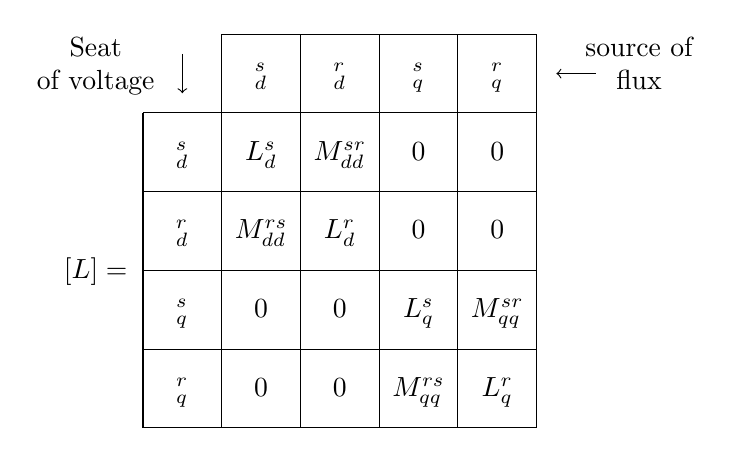
\begin{tikzpicture} [anchor = base, baseline =0pt]
        \draw (0,0)--(5,0) (0,1)--(5,1) (0,2)--(5,2) (1,3)--(5,3) (0,-1)--(5,-1) (0,-2)--(5,-2);
        \draw (0,-2)--(0,2) (1,-2)--(1,3) (2,-2)--(2,3) (3,-2)--(3,3) (4,-2)--(4,3) (5,-2)--(5,3);
        \draw (0.5,-1.6) node{$_q^r$} +(0,1) node{$_q^s$} +(0,2) node{$_d^r$} +(0,3) node{$_d^s$};
        \draw (1.5,-1.6) node{0} +(0,1) node{0} +(0,2) node{$M_{dd}^{rs}$} +(0,3) node{$L_d^s$}+(0,4) node{$_d^s$};
        \draw (2.5,-1.6) node{0} +(0,1) node{0} +(0,2) node{$L_{d}^{r}$} +(0,3) node{$M_{dd}^{sr}$}+(0,4) node{$_d^r$};
        \draw (3.5,-1.6) node{$M_{qq}^{rs}$} +(0,1) node{$L_q^s$} +(0,2) node{0} +(0,3) node{0}+(0,4) node{$_q^s$};
        \draw (4.5,-1.6) node{$L_q^r$} +(0,1) node{$M_{qq}^{sr}$} +(0,2) node{0} +(0,3) node{0}+(0,4) node{$_q^r$};
        \draw (-0.6,-0.1) node{$[L] =$};
        \draw [align = center,->](-0.6, 2.3) node{Seat\\of voltage} (0.5,2.75)--(0.5, 2.25);
        \draw [align = center,->](6.3, 2.3) node{source of\\flux} (5.75,2.5)--(5.25,2.5);
    \end{tikzpicture}
\end{equation}

The matrix contains mutual inductance coefficients forming equal pairs
\begin{align*}
    M_{dd}^{sr} & = M_{dd}^{rs} \\
    M_{qq}^{sr} & = M_{qq}^{rs}
\end{align*}
For a salient-pole machine
\begin{equation*}
    L_d^s \neq L_q^s , \quad L_d^r \neq L_q^r \text{and} M_{dd}^{sr} \neq M_{qq}^{sr}
\end{equation*}
as the $d$-axis and $q$-axis permeances are different. The corresponding inductances are equal for a machine with zero saliency.

\vspace{2em}

\noindent (b) \emph{The rotational coefficient matrix} $[G]$\\
The $[G]$ matrix in general form
\begin{equation}
    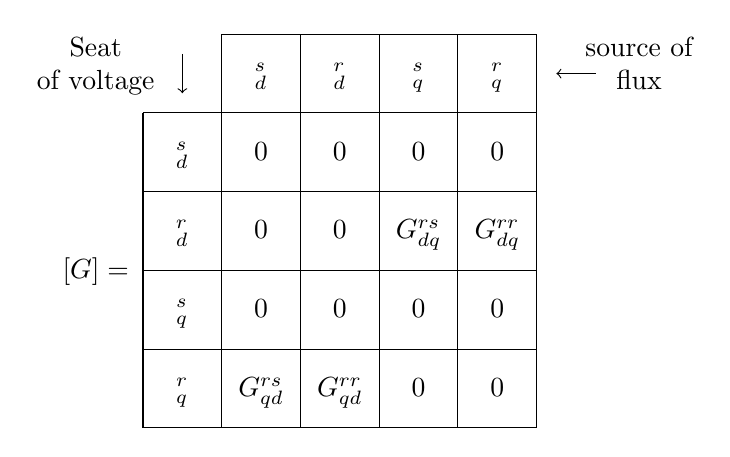
\begin{tikzpicture} [anchor = base, baseline =0pt]
        \draw (0,0)--(5,0) (0,1)--(5,1) (0,2)--(5,2) (1,3)--(5,3) (0,-1)--(5,-1) (0,-2)--(5,-2);
        \draw (0,-2)--(0,2) (1,-2)--(1,3) (2,-2)--(2,3) (3,-2)--(3,3) (4,-2)--(4,3) (5,-2)--(5,3);
        \draw (0.5,-1.6) node{$_q^r$} +(0,1) node{$_q^s$} +(0,2) node{$_d^r$} +(0,3) node{$_d^s$};
        \draw (1.5,-1.6) node{$G_{qd}^{rs}$} +(0,1) node{0} +(0,2) node{0} +(0,3) node{0}+(0,4) node{$_d^s$};
        \draw (2.5,-1.6) node{$G_{qd}^{rr}$} +(0,1) node{0} +(0,2) node{0} +(0,3) node{0}+(0,4) node{$_d^r$};
        \draw (3.5,-1.6) node{0} +(0,1) node{0} +(0,2) node{$G_{dq}^{rs}$} +(0,3) node{0}+(0,4) node{$_q^s$};
        \draw (4.5,-1.6) node{0} +(0,1) node{0} +(0,2) node{$G_{dq}^{rr}$} +(0,3) node{0}+(0,4) node{$_q^r$};
        \draw (-0.6,-0.1) node{$[G] =$};
        \draw [align = center,->](-0.6, 2.3) node{Seat\\of voltage} (0.5,2.75)--(0.5, 2.25);
        \draw [align = center,->](6.3, 2.3) node{source of\\flux} (5.75,2.5)--(5.25,2.5);
    \end{tikzpicture}
\end{equation}

It is seen that $G$ coefficients are only obtained for pseudo-stationary rotor coils. Coils acting as flux sources may be stator or pseudo-stationary rotor coils.

The significance of the $G$ coefficients is determined from
\begin{equation*}
    G_{rs} = -M_m \sin \theta_r
\end{equation*}

The value of $M_m$ is the coupling obtained when the axis of the seat of voltage coil is imagined to be aligned with the axis of the source of flux coil.

Coefficients with stator coils as the source of flux
\begin{align*}
    G_{dq}^{rs} &= - M_{qq}^{rs} \sin \Big (+\frac{\pi}{2}\Big) = -M_{qq}^{rs}\\
    G_{qd}^{rs} &= - M_{dd}^{rs} \sin \Big (-\frac{\pi}{2}\Big) = -M_{dd}^{rs}
\end{align*}

Coefficients involving two pseudo-stationary coils 
\begin{align*}
    G_{dq}^{rr} & =-M_{qq}^{rr} \sin \Big( +\frac{\pi}{2} \Big) = -M_{qq}^{rr}\\
    G_{qd}^{rr} & =-M_{dd}^{rr} \sin \Big( -\frac{\pi}{2} \Big) = -M_{dd}^{rr}\\
    M_{qq}^{rr} & = \sqrt{L_q^r L_q^r} = L_q^r \\
    M_{dd}^{rr} & = \sqrt{L_d^r L_d^r} = L_d^r
\end{align*}

Substituting the above inductance coefficients in (5.81)
\begin{equation}
    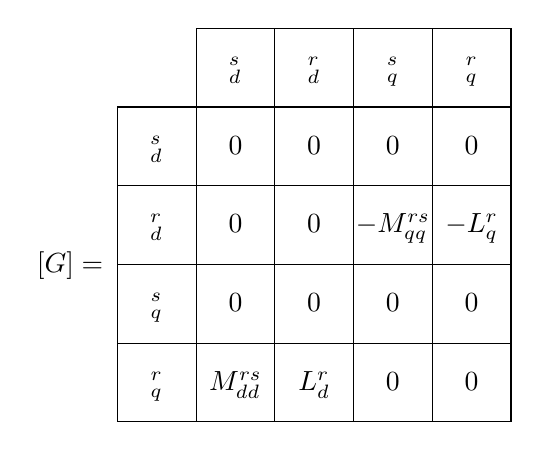
\begin{tikzpicture} [anchor = base, baseline =0pt]
        \draw (0,0)--(5,0) (0,1)--(5,1) (0,2)--(5,2) (1,3)--(5,3) (0,-1)--(5,-1) (0,-2)--(5,-2);
        \draw (0,-2)--(0,2) (1,-2)--(1,3) (2,-2)--(2,3) (3,-2)--(3,3) (4,-2)--(4,3) (5,-2)--(5,3);
        \draw (0.5,-1.6) node{$_q^r$} +(0,1) node{$_q^s$} +(0,2) node{$_d^r$} +(0,3) node{$_d^s$};
        \draw (1.5,-1.6) node{$M_{dd}^{rs}$} +(0,1) node{0} +(0,2) node{0} +(0,3) node{0}+(0,4) node{$_d^s$};
        \draw (2.5,-1.6) node{$L_{d}^{r}$} +(0,1) node{0} +(0,2) node{0} +(0,3) node{0}+(0,4) node{$_d^r$};
        \draw (3.5,-1.6) node{0} +(0,1) node{0} +(0,2) node{$-M_{qq}^{rs}$} +(0,3) node{0}+(0,4) node{$_q^s$};
        \draw (4.5,-1.6) node{0} +(0,1) node{0} +(0,2) node{$-L_{q}^{r}$} +(0,3) node{0}+(0,4) node{$_q^r$};
        \draw (-0.6,-0.1) node{$[G] =$};
        %\draw [align = center,->](-0.6, 2.3) node{Seat\\of voltage} (0.5,2.75)--(0.5, 2.25);
        %\draw [align = center,->](6.3, 2.3) node{source of\\flux} (5.75,2.5)--(5.25,2.5);
    \end{tikzpicture}
\end{equation}

Combining the results obtained in (5.80) and (5.82), substituting in the general voltage equation
\begin{equation*}
    [v] = \{[R] + [L]p+\omega_r[G]\}[i]
\end{equation*}
gives the complete impedance matrix for a four-coil, primitive machine, Fig.\ 5.18.
\begin{equation}
    \begin{bmatrix}
        v_d^s \\ v_d^r \\ v_q^s \\ v_q^r
    \end{bmatrix}
    =
    \begin{bmatrix}
        (R_d^s + L_d^s p) & M_{dd}^{rs}p & 0 & 0\\
        M_{dd}^{rs}p & (R_d^r + L_d^r p) & -\omega_r M_{qq}^{rs} &-\omega_r L_q^r \\
        0 & 0 & (R_q^s + L_q^s p) & M_{qq}^{rs} p \\
        \omega_r M_{dd}^{rs} & \omega_r L_{d}^{r} & M_{qq}^{rs} p & (R_q^r + L_q^r p)
    \end{bmatrix}
    \begin{bmatrix}
        i_d^s \\ i_d^r \\ i_q^s \\ i_q^r
    \end{bmatrix}
\end{equation}
\subsection{Torque and power}

Substituting (5.82) in (5.74)
\begin{equation}
    T_e = (\text{pole-pairs})
    \begin{bmatrix}
        i_d^s & i_d^r &i_q^s & i_q^r
    \end{bmatrix}
    \begin{bmatrix}
        0 & 0 & 0 & 0 \\
        0 & 0 & -M_{qq}^{rs} & -L_q^r \\
        0 & 0 & 0 & 0 \\
        M_{dd}^{rs} & L_d^r & 0 & 0 
    \end{bmatrix}
    \begin{bmatrix}
        i_d^s \\  i_d^r \\ i_q^s \\ i_q^r
    \end{bmatrix}
\end{equation}
Expanding and collecting terms
\begin{equation}
    T_e = (\text{pole-pairs}) [M_{dd}^{rs} i_d^s i_q^r - M_{qq}^{rs} i_q^s i_d^r + (L_d^r  - L_q^r)i_d^r i_q^r]
\end{equation}
The torque component in $(L_d^r - L_q^r)$ is only present in salient-pole machines and is called saliency-torque. The remaining torque components, which define the electromagnetic torque for a uniform air-gap, are described as cylindrical torques. It will be noted that the cylindrical torque components comprise a positive motoring term and a negative generating term; the sum of all such terms determines the machine action, motor, or generator.

The total internal electrical power developed by the machine
\begin{equation}
    P_e = \frac{\omega_r}{(\text{pole-pairs})} T_e
\end{equation}
\begin{equation}
    P_e = \omega_r [M_{dd}^{rs} i_d^s i_q^r - M_{qq}^{rs} i_q^s i_d^r + (L_d^r  - L_q^r)i_d^r i_q^r]
\end{equation}

An alternative method of deriving (5.85) is to consider the torque exerted of each pseudo-stationary coil by all coils at right-angles.
\chapter{D.C.\ and crossfield machines}
The physical arrangement of a d.c.\ or crossfield machine is identical to the primitive machine. The rotating commutator winding has one or more brush-pairs on orthogonal axes and stator coils are on the same orthogonal axes. The equation developed in chapter 5 for a primitive machine are directly applicable for these types of machines.
\section{General analysis}
Machine voltage and torque equations my be written down by inspection when the ideas and rules in chapter 5 are understood. For convenience, a two pole machine is always schematically shown although the equations apply for any number of pole-pairs.
Consider a machine with one brush-pair on the quadrature-axis and two direct-axis stator coils as shown in Fig.\ 6.1. The voltage and electromagnetic torque equations are:

\begin{equation}
    \begin{bmatrix}
        v_d^{s1}\\[2ex] v_d^{s2}\\[2ex] v_q^{r1}
    \end{bmatrix} =
    \begin{bmatrix}
        (R_d^{s1} + L_d^{s1}p) & M_{d}^{s1}{}_{d}^{s2} p & 0 \\[2ex]
        M{_d^{s2}{}_d^{s1}} & (R_d^{s2} + L_d^{s2}p) & 0 \\[2ex]
        \omega_r G_{q}^{r1}{}_d^{s1} & \omega_r G_{q}^{r1}{}_d^{s2} & (R_q^r1{} + L_q^{r1}p)
    \end{bmatrix}
    \begin{bmatrix}
        i_d^{s1} \\[2ex] i_d^{s2} \\[2ex] i_q^{r1}
    \end{bmatrix}
    \label{}
\end{equation}
\begin{equation}
    T_e = (\text{pole-pairs})[i_q^{r1}(G_q^{r1}{}_d^{s1} i_d^{s1} + G_q^{r1}{}_d^{s2} i_d^{s2})]
    \label{}
\end{equation}

The rotational inductance ($G$) coefficients mat be replaced by transformer inductance ($M$) coefficients as described in section 5.5.

\begin{equation}
    \begin{bmatrix}
        v_d^{s1}\\[2ex] v_d^{s2}\\[2ex] v_q^{r1}
    \end{bmatrix} =
    \begin{bmatrix}
        (R_d^{s1} + L_d^{s1}p) & M_{d}^{s1}{}_{d}^{s2} p & 0 \\[2ex]
        M{_d^{s2}{}_d^{s1}} & (R_d^{s2} + L_d^{s2}p) & 0 \\[2ex]
        \omega_r M_{d}^{r1}{}_d^{s1} & \omega_r M_{d}^{r1}{}_d^{s2} & (R_q^r1{} + L_q^{r1}p)
    \end{bmatrix}
    \begin{bmatrix}
        i_d^{s1} \\[2ex] i_d^{s2} \\[2ex] i_q^{r1}
    \end{bmatrix}
    \label{}
\end{equation}

\begin{equation}
    T_e = (\text{pole-pairs})[i_q^{r1}(M_d^{r1}{}_d^{s1} i_d^{s1} + M_d^{r1}{}_d^{s2} i_d^{s2})]
    \label{}
\end{equation}
Assuming a mechanical damping coefficient $D$ proportional to speed, the torque balance equation is.

\begin{equation}
    T_m + T_e = J p \omega_m + D \omega_m
    \label{}
\end{equation}
where, as previously, suffix $m$ refers to a mechanical quantity and $J$ is the polar moment of inertia.

The general equations (6.3) to (6.5) apply for steady-state or transient performance. For steady-state operation the derivative terms are zero and the equations are considerably simplified.

For simultaneous changes of current and speed the solution of the equations may be extremely formidable, see Section 6.4.3.
\noindent \textit{Simplified notation} In the previous chapter each primitive coil is identified by two letters and a number. With a particular machine arrangement it is more convenient to use a single letter to identify a winding, especially with d.c.\ and crossfield machines in which primitive coils correspond to actual windings.

For example, a coil designated $f$ has resistance $r_f$, self-inductance $L_f$, and its mutual inductance with a coil $s$ is $M_{sf}$.

\section{D.C.\ machine steady state analysis}
D.C.\ machines have one or more stator windings for the required load characteristic. Additional stator windings are included to give satisfactory commutation.

\subsection{Field windings}
The main stator or field windings are wound on salient poles. Coils may be connected:
\begin{enumerate}
    \item in series with the rotor or armature winding, \\
        i.e.\ \textit{a series field}
    \item[or \stepcounter{enumi} (\alph{enumi})] energized from a separate d.c.\ supply, \\
        i.e.\ a \textit{separately-excited field}
    \item[or \stepcounter{enumi} (\alph{enumi})] across the armature brush-pair,\\
        i.e.\ a \textit{shunt field.}
\end{enumerate}
A d.c.\ motor with a shunt winding is identical to a separately-excited machine as in both cases the winding is energized from the supply voltage.

With a shunt generator, the simplifying assumption of a linear flux/current relationship is not justified as the open-circuit voltage is limited only by magnetic saturation. The analysis of this machine therefore requires a more realistic treatment, see Section 6.2.4.
A \textit{compound machine} has a series field together with a shunt or separately-excited field winding. The following analysis is for a compound machine with series and separately-excited windings.
\subsection{Compound machine analysis}
Figure 6.2(a) shows the primitive coil arrangement for a compound machine. For simplicity, the armature and the series and separately-excited fields are designated $a$, $s$ and $f$, respectively. The primitive voltage equations are,

\begin{equation}
    \begin{bmatrix}
        v_d^{s2}\\[2ex] v_d^{s1}\\[2ex] v_q^{r1}
    \end{bmatrix} =
    \begin{bmatrix}
        (R_f + L_f p) & M_{fs} p & 0 \\[2ex]
        M_{sf} & (R_s + L_s p) & 0 \\[2ex]
        \omega_r M_{af} & \omega_r M_{as} & (R_a + L_a p)
    \end{bmatrix}
    \begin{bmatrix}
        i_d^{s2} \\[2ex] i_d^{s1} \\[2ex] i_q^{r1}
    \end{bmatrix}
    \label{}
\end{equation}

The field coils may be connected to give m.m.f.s in the same sense or in opposition to each other, and are termed either \textit{cumulative connected} or \textit{differential connected} windings, respectively. The two alternative connections for a machine in the motoring mode are shown in Figs.\ 6.2(b) and 6.2(c).
Reversal of the armature current also reverses the series field, and a differential connected motor operates as a cummulative connected generator. Similarly, a cumulative connected motor operates as a differential connected generator.

Establishing relationships between the primitive and the actual machine currents and voltages,
\begin{align*}
    i_q^{r1} & = i_a & v_q^{r1} & = v_a \\[2ex]
    i_d^{s1} & = \pm i_a & v_d^{s1} & = v_s \\[2ex]
    i_d^{s2} & = i_f & v_d^{s2} & = v_f
\end{align*}

In all cases the current $i_a$ is shown entering coil $a$ at the dot. For motor action,$i_a$ is a positive quantity and for generator action is a negative quantity.

The armature circuit voltage $V=v_a\pm v_s$, thus
\begin{equation*}
    V=v_q^{r1} \pm v_d^{s1}
    \label{}
\end{equation*}

Substituting in (6.6) for the primitive voltages and currents, combining $v_q^{r1}$ and $v_d^{s1}$ and writing $R = R_a + R_s$, $L = L_a + L_s$,

\begin{equation}
    \begin{bmatrix}
        v_f \\[2ex] V
    \end{bmatrix} =
    \begin{bmatrix}
        (R_f +F_f p) & \pm M_{sf} p \\[2ex]
        (\omega_r M_{af} \pm M_{sf} p) & (R + L p \pm \omega_r M_{as})
    \end{bmatrix}
    \begin{bmatrix}
        i_f \\[2ex] i_a
    \end{bmatrix}
    \label{}
\end{equation}

The electromagnetic torque equation is,
\begin{equation*}
    T_e = (\text{pole-pairs})[i_q^{r1} i_d{s2} M_{af} + i_q^{r1} i_d^{s1} M_{as}]
\end{equation*}
Substituting for actual currents,
\begin{equation}
    T_e = (\text{pole-pairs})[i_a M_{af} i_f \pm i_a^{2} M_{as}]
    \label{}
\end{equation}

The alternative sign $\pm$ is positive for a cumulative connected motor and a differential connected generator, and for a differential connected motor and a cummulative connected generator.

\subsection{Steady-state analysis}
The steady-state operation of a compound machine is determined from the general performance equations. By omitting the appropriate winding from the current results for the compound machine, steady-state solutions for series and separately-excited machines are readily obtained.

\subsubsection{\textit{Compound machine}}
With constant speed and current values the $p \omega_r$ and $p i$ terms are zero, and (6.7), (6.8) and (6.5) may be written,
\begin{align}
    V & =\omega_r M_{af} I_f + (R \pm \omega_r M_{as}) I_a \\[2ex]
    T_e & = (\text{pole-pairs})[I_a M_{af} i_f \pm I_a^2 M_{as}] \\[2ex]
    T_m + T_e & = D \omega_m
\end{align}

Typical characteristics are shown for a compound machine in Fig.\ 6.3. A \textit{level-compounded} generator has  no voltage regulation.

\noindent In practice, saturation of the magnetic circuit increases the voltage regulation at high load currents and the term level-compounded describes a generator with zero voltage regulation at full load.

\subsubsection{\textit{Series machine}}
Omitting the separately-excited winding gives the steady-state equations for a series motor
\begin{align}
    V & = (R + \omega_r M_{as}) I_a\\[2ex]
    T_e & = (\text{pole-pairs})(I_a^2 M_{as})
    \label{}
\end{align}
The characteristics for a series motor, Fig.\ 6.4.\ show a high starting torque and the danger of running the machine on no-load. The series generator is seldom employed.

\subsubsection{\textit{Separately-excited machine or shunt motor}}
The steady-state equations are:
\begin{align}
    V & = R_a I_a + \omega_r M_{af} I_f\\[2ex]
    T_e & = (\text{pole-pairs})(I_a M_{af} I_f)
    \label{}
    \label{}
\end{align}

Typical characteristics are shown in Fig.\ 6.5.

\subsection{Shunt generator}
The assumption made in the previous work may give raise to appreciable errors in analysing the performance of d.c.\ machines. However, the ability to derive and solve general equations for both steady-state and transient behaviour often justifies these assumptions. With these simplifying assumptions the performance of the shunt generator cannot be determined. The analysis of this machine requires a more realistic approach employing the
flux/excitation m.m.f.\ characteristic.
\subsubsection{\textit{Actual characteristics}}
The field current for a shunt generator is supplied by the armature voltage, see Fig.\ 6.6. With the armature rotating the residual flux in the stator poles generates a voltage across the brush-pair which drives current through the field winding increasing the pole flux, and hence, the armature voltage. The voltage continues to rise in a fairly linear manner with field current and the machine is said to self-excite. When the magnetic circuit of the pole flux
begins to saturate, the output voltage does not increases as rapidly as previously, see Fig.\ 6.7. A point is reached at which the voltage characteristic cuts the field resistance line and this corresponds to the open-circuit voltage of the machine.

Two necessary conditions for self-excitation are,
\begin{enumerate}
    \item the residual flux is in the \textit{correct sense}, i.e., field current due to rotational voltage reinforces the residual flux of the stator poles; and
    \item the slope of the field resistance line is sufficiently low to intersect the voltage characteristic at a reasonable value above the knee of the curve.
\end{enumerate}
For a given speed the \textit{critical field resistance} is the maximum value of field circuit resistance at which self-excitation occurs. With a given value of field circuit resistance there is a  \textit{critical speed} below which the machine fails to excite. The sudden short-circuit of an energized shunt generator reduces the excitation to zero and the steady-state value of short-circuit current, due only to residual pole flux, is small.

The solution of shunt generator problems requires graphical methods unless the magnetization characteristic can be expressed as an analytic function of the field current.

\subsubsection{\textit{Method of analysis}}
The non-linear voltage characteristic of a shunt generator, Fig.\ 6.7, may be represented wit reasonable accuracy by two linear parts of different slope as Fig.\ 6.8.

With \textit{incremental inductance coefficients} of $G_{af}^m$, $M_{af}^m$ and $G_{af}^n$, $M_{af}^n$ for the two slopes, the rotational voltage term in the armature coil is given by

\begin{align*}
    i_{f1} \geq i_f > 0, \hspace{8em}\\
    \text{rotational voltage term} & =\omega_r G_{af}^m i_f \\
    & = \omega_r M_{af}^m i_f\\
    i_f > i_{f1}, \hspace{10em} &\\
    \text{rotational voltage term} & = \omega_r [G_{af}^m i_{f1} + G_{af}^n (i_f - i_{f1})] \\
    &=  \omega_r [M_{af}^m i_{f1} + M_{af}^n (i_f - i_{f1})]
\end{align*}

The voltage and torque equations in the operating region above the knee of the curve, part $n$, are

\begin{align}
    v & = (R_a + L_a p)i_a + \omega_r M_{af} i_f \\
    v_f = v & = (R_f + L_f p) i_f\\
    T_e & = (\text{pole-pairs})(M_{af} i_a i_f)
    \label{}
\end{align}

As a function of $i_f$,

\begin{equation*}
    M_{af} = M_{af}^n + \frac{i_{f1}(M_{af}^m - M_{af}^n)}{i_f}
\end{equation*}

Eliminating $i_f$ from (6.16) and (6.17),

\begin{equation}
    v = \frac{(R_a + L_a p) i_a + \omega_r i_{f1} (M_{af}^m - M_{af}^n)}{1 - \dfrac{\omega_r M_{af}^n}{R_f + L_f p}} 
    \label{}
\end{equation}

For steady-state operation,

\begin{equation}
    v = \frac{R_a i_a + \omega_r i_{f1}(M_{af}^m - M_{af}^n)}{1 - \dfrac{\omega_r M_{af}^n}{R_f}}
    \label{}
\end{equation}

Equations (6.19) and (6.20) are valid for operation in region $n$ only, corresponding to a range of field current $i_f \geq i_{f1}$.

\subsection{Compensating winding}
A d.c.\ machine with a severely fluctuating load, e.g.\ a rolling mill motor, may flashover across the commutator segments due to the high voltages induced in the armature coils by the rapidly changing armature current. A flashover often results in severe damage as short-circuit current may flow along the breakdown path. The large voltages induced in the armature coils may be eliminated by including a \textit{compensating winding} in the machine.

The voltage induced between two adjacent commutator segments depends on the rate of flux-linkage with the armature coil connected to the segments. There is an induced voltage (nearly independent of load current) due to the main excitation flux (an $\omega_r M$ term). An additional induced voltage may appear due to a rapid change of armature current and, hence, self-linkage (an $L p i$ term).

The compensating winding, connected in series with the armature, produces an m.m.f.\ equal and opposite to that of the armature, see Fig.\ 6.9(a). A rapid change of load current produces negligible change of flux along the $q$-axis, inducing little voltage in the armature coils.

Representing a separately-excited machine with a compensating winding as a primitive machinem Fig.\ 6.9(b), the coil voltages are
\begin{equation}
    \begin{bmatrix}
        v_d^{s1} \\[2ex] v_q^{s1} \\[2ex] v_q^{r1}
    \end{bmatrix} = 
    \begin{bmatrix}
        (R_f + L_f p) & 0 & 0 \\[2ex]
        0 & (R_c + L_c p) & M_{ca} \\[2ex]
        \omega_r M_{af} & M_{ca} p & (R_a + L_a p)
    \end{bmatrix}
    \begin{bmatrix}
        i_d^{s1} \\[2ex] i_q^{s1} \\[2ex] i_q{r1}
    \end{bmatrix}
    \label{}
\end{equation}

Connecting the armature and compensating windings,
\begin{align*}
    &\text{armature current}  & i_a & = i_q^{r1} = -i_q^{s1} \\
    &\text{armature circuit voltage} & v & = v_q^{r1} - v_q^{s1}
    \label{}
\end{align*}
equation (6.21) may be written

\begin{equation}
    \begin{bmatrix}
        v_f \\[2ex] v
    \end{bmatrix} =
    \begin{bmatrix}
        (R_f + L_f p) & 0 \\[2ex]
        \omega_r M_{af} & (R_a + R_c) + (L_a + L_c -2 M_{ac})p
    \end{bmatrix}
    \begin{bmatrix}
        i_f \\[2ex] i_a
    \end{bmatrix}
    \label{}
\end{equation}

Equations (6.22) are identical to those for a separately-excited machine with an armature resistance and inductance of ($R_a + R_c$) and ($L_a + L_c - 2M_{ac}$), respectively. With equal turns on the armature and compensating windings,
\begin{equation*}
    L_a \bumpeq L_c \bumpeq M_{ac}
\end{equation*}
and the effective armature inductance ($L_a + L_c - 2M_{ac}$) is negligible.

With the compensating winding not extending to the interpolar regions, as shown in Fig.\ 6.9(a), i.e., restricted to the pole faces, the compensating winding inductance is less than the armature self-inductance and the effective armature inductance ($L_a + L_c - 2M_{ac}$) may not be negligible.

\subsection{Interpole windings}
Satisfactory commutator action requires the current in a coil undergoing commutation to reverse in the commutation period, see Fig.\ 6.10. An induced voltage, produced by changing self-flux in the coil, opposes the current change and may prevent complete current reversal in the time allowed for commutation.

The difficulty is overcome in all modern machines by fitting \textit{interpoles} to give practically spark-free commutation at all loads and speeds. Interpoles, located s their name suggest in the interpolar region, see Fig.\ 6.11(a), are connected in series with the armature winding and produces fluxed which induce voltages in the coils undergoing commutation. These voltages are approximately equal and opposite to the self-induced voltages and enable the current to reverse
completely in the commutation period. Both self-induced and interpole induced voltages are proportional to speed and armature current, hence correct compensation is achieved for all values of speed and load, including rotation in either direction.

The interpole acts as a compensating winding over a small angle and is sometimes termed a \textit{commutating pole} or \textit{compole}.

The analysis is identical for machines with interpoles or compensating windings. However, the inductance of a interpole winding, $L_i$, is small compared with the armature inductance, $L_a$, and the modified armature circuit inductance ($L_a + L_i - 2M_{ai}$) cannot be ignored.

Interpoles are necessary for a machine with a compensating winding restricted to the salient-pole faces but are not required for a compensating winding which extends over the interpolar regions.

\subsection{Starting}
With full voltage applied to a stationary d.c.\ machine, the armature current, limited only by the low resistance of the armature circuit, would be dangerously large. Consequently, d.c.\ motors are always started at reduced armature voltage. A common method is additional resistance  in series with the armature which can be gradually removed as the speed increases. Full field current is applied to shunt machines to provide maximum rotational voltage as soon as possible. A typical
starter resistor has several sections which are cut out in turn as the motor increases speed. The current rises to a maximum shortly after switching-on and decays slowly as the armature rotational voltage build up with speed. On cutting-out the first resistor section the current increases rapidly to a peak value and then decays again. This is repeated until all starting resistance is out of circuit. The resistor sections are designed to limit the current maxima to a suitable
value provided that sufficient time is allowed for the current to fall to a certain minimum level before the next section is cut out. The problem is considered in more detail in Section 6.4.

\section{Sudden short-circuit of a d.c.\ generator}
The voltage and torque equations describing the performance of a machine are completely general and apply to transient as well as steady-state behaviour. As an example of transient analysis consider the sudden short-circuit of a d.c.\ generator with differential series and separately-excited field windings. The voltage equations are identical to those derived in Section 6.2.1 for the cumulative compound motor represented schematically in Fig.\ 6.2(b)
\begin{equation}
    \begin{bmatrix}
        v_f \\[2ex] v
    \end{bmatrix} =
    \begin{bmatrix}
        (R_f + L_f p) & M_{sf} p \\[2ex]
        (M_{sf} p + \omega_r M_{af}) & (R + L p + \omega_r M_{as})
    \end{bmatrix}
    \begin{bmatrix}
        i_f \\[2ex] i_a
    \end{bmatrix}
    \label{}
\end{equation}
Assuming no change of speed, i.e.\ $\omega_r$ is constant, the simultaneous linear differential equations (6.23) are readily solved using Laplace transforms.

\subsection{Analysis for a machine on load}
Consider a short-circuit at time $t=0$ on the output terminals of a generator with differential series and separately-excited field windings. The field voltage $V_f$ and the speed $\omega_r$ are assumed constant.
\begin{align*}
    \text{Pre-fault conditions}, t < 0\\
    & \text{armature (and series field) current } &= \mathring{I}_a\\
    & \text{output voltage} & = \mathring{V}\\
    & \text{field current} & = \mathring{I}_f\\
    \text{Fault condition}, t \geq 0 \\
    & \text{armature current, time-dependent} & = i_a\\
    & \text{field current, time-dependent} & = i_f \\
    & \text{output voltage} & = 0
\end{align*}

Substituting initial conditions in the voltage equations (6.23)
\begin{equation}
    \mathring{V} = \omega_r M_{af} \mathring{I}_f + R \mathring{I}_a + \omega_r M_{as} \mathring{I}_a
    \label{}
\end{equation}
(\textit{Note:} the current $\mathring{I}_a$ will be a negative quantity as the machine is generating.)

Transforming (6.23) by Laplace to the $\mathbf s$ domain and including initial conditions,
\begin{align}
    \bar v_f & = (R_f + L_f \mathbf{s})\bar i_f - L_f \mathring I_f + M_{sf} \mathbf{s} \bar i_a - M_{sf} \mathring I_a \nonumber \\ %chktex 7
    \bar v & = (M_{sf} \mathbf{s} + \omega_r M_{af} )\bar \imath_f - M_{sf} \mathring I_f + (R + L \mathbf{s} + \omega_r M_{as})\bar i_a - L\mathring I_a %chktex 7
    \label{}
\end{align}

In matrix notation (6.25) may be written with the initial conditions grouped together,
\begin{multline}
    \begin{bmatrix}
        \bar v_f \\[2ex] \bar v
    \end{bmatrix} = 
    \begin{bmatrix}
        (R_f + L_f \mathbf{s} ) & M_{sf}\mathbf s  \\[2ex]
        (M_{sf} \mathbf{s} + \omega_r M_{af} ) & (R + L\mathbf{s}+\omega_r M_{as} )
    \end{bmatrix}
    \begin{bmatrix}
        \bar i_f \\[2ex] \bar i_a %chktex 7
    \end{bmatrix} \\
    - 
    \begin{bmatrix}
        L_f & M_{sf} \\[2ex]
        M_{sf} & L
    \end{bmatrix}
    \begin{bmatrix}
        \mathring I_f \\[2ex] \mathring I_a
    \end{bmatrix}
\end{multline}
With initial conditions transferred to the left-side,
\begin{equation}
    \begin{bmatrix}
        \bar v_f + L_f \mathring I_f + M_{sf} \mathring I_a \\[2ex]
        \bar v + M_{sf} \mathring I_f + L \mathring I_a
    \end{bmatrix}
    =
    \Bigg[ Z(\mathbf s)\Bigg]
    \begin{bmatrix}
        \bar i_f \\[2ex] \bar i_a %chktex 7
    \end{bmatrix}
    \label{}
\end{equation}
Now
\begin{equation*}
    \begin{array}{r@{\;=\;}ll}
        \bar v & 0 & \text{for } t \geq 0 \text{, machine short-circuited} \\
        \bar v_f & \dfrac{V_f}{\mathbf s} &\text{as } v_f \text{\ is constant.}
    \end{array}
\end{equation*}
Equation (6.27) may be written,
\begin{equation}
    \begin{bmatrix}
        \dfrac{V_f}{\textbf{s}} + L_f \mathring I_f + M_{sf} \mathring I_a \\[2ex]
        M_{sf} \mathring I_f + L \mathring I_a
    \end{bmatrix}
    =
    \Bigg[ Z(\textbf{s})\Bigg]
    \begin{bmatrix}
        \bar i_f \\ \bar i_a %chktex 7
    \end{bmatrix}
    \label{}
\end{equation}

The solution for the transient currents $i_a(t)$ and $i_f(t)$ may be obtained using inverse Laplace transforms.

\subsection{Solution for unloaded machine}
With $\mathring I_a =0$, (6.28) and (6.24) reduce to
\begin{equation}
    \begin{bmatrix}
        V_f/\textbf{s} + L_f \mathring I_f \\[2ex]
        M_{sf} \mathring I_f 
    \end{bmatrix}
    =
    \Bigg[ Z(\textbf{s})\Bigg]
    \begin{bmatrix}
        \bar i_f \\ \bar i_a %chktex 7
    \end{bmatrix}
    \label{}
\end{equation}
\begin{equation}
    \mathring V = \omega_r M_{af} \mathring I_f
    \label{}
\end{equation}
Combining (6.29) and (6.30) and eliminating $i_f$,

\begin{equation}
    \bar i_a = - \dfrac{(\mathring V/\mathbf s)(R_f + L_f \mathbf s)}{(R + \omega_r M_{as}+L \mathbf s)(R_f + L_f \mathbf s) - M_{sf} \textbf{s} ( M_{sf} \textbf{s} + \omega_r M_{af})} %chktex 7
    \label{}
\end{equation}
Writing $\tau$ for $L / (R + \omega_r M_{as})$ and $\tau_f$ for $L/R_f$ in (6.31),
\begin{multline}
    \bar i_a = - \dfrac{\mathring V(1-\textbf{s}\tau_f)}{\textbf{s}(R + \omega_r M_{as}) \bigg\{1 + \textbf{s} \bigg[\tau + \tau_f - \dfrac{\omega_r M_{af} M_{sf}}{R_f (R + \omega_r M_{as})} \bigg]} \\ %chktex 7
    + \textbf{s}^2 \bigg[\tau \tau_f - \dfrac{M_{sf}^2}{R_f(R + \omega_r M_{as})}\bigg]\bigg\}
    \label{}
\end{multline}

\begingroup
\setlength{\lineskip}{2pt} 
\noindent Now $\dfrac{M_{sf}}{R_f(R + \omega_r m_{af})}$ may be written $\dfrac{K_{sf}^2}{(R + \omega_r M_{as}) R_f}$ \\
\phantom{Now }$= \tau \tau_f k_{sf}^2 \dfrac{L_s}{L}$ where $k_{fs}$ is the coefficient of coupling.\\

\endgroup
\noindent Substituting in (6.32)
\begin{multline}
    \bar i_a = - \dfrac{\mathring V(1-\textbf{s}\tau_f)}{\textbf{s}(R + \omega_r M_{as}) \bigg\{1 + \textbf{s} \bigg[\tau + \tau_f - \dfrac{\omega_r M_{af} M_{sf}}{R_f (R + \omega_r M_{as})} \bigg]} \\ %chktex 7
    + \textbf{s}^2 \bigg[\tau \tau_f \bigg(1 - \dfrac{k_{sf}^2 L_s}{L}\bigg)\bigg]\bigg\}
    \label{}
\end{multline}
Expressed in partial fraction form
\begin{equation}
    \bar i_a = - \dfrac{\mathring V}{\textbf{s}(R + \omega_r M_{as})} \dfrac{(A^2 - B^2)(1 + \mathbf s \tau_f)}{(\mathbf s + A + B)(\textbf{s} + A - B)} %chktex 7
    \label{}
\end{equation}
where
\begin{equation}
    A = \dfrac{1}{2 \tau \tau_f \bigg(1 - \dfrac{k_{sf}^2 L_s}{L}\bigg)} \bigg[\tau_f + \tau - \dfrac{\omega_r M_{af} M_{sf}}{R_f (R + \omega_r M_{as})}\bigg]
    \label{}
\end{equation}
and
\begin{equation}
    B^2 = A^2 - \dfrac{1}{\tau \tau_f \bigg(1 - \dfrac{k_{sf}^2 L_s}{L}\bigg)}
    \label{}
\end{equation}
Expanding (6.34)
\begin{multline}
    \bar i_a = - \dfrac{\mathring V}{(R + \omega_r M_{as})}\bigg\{\dfrac{1}{\mathbf{s}} + \big(\dfrac{A-B}{2B}\bigg) \bigg[\dfrac{1 - (A + B)\tau_f}{\mathbf{s} + A + B}\bigg] \\ %chktex 7
    - \bigg(\dfrac{A+B}{2B}\bigg)\bigg[\frac{1 - (A - B)\tau_f}{\mathbf{s}+A-B}\bigg]\bigg\} 
    \label{}
\end{multline}
Transforming
\begin{multline}
    \bar i_a(t) = - \dfrac{\mathring V}{(R + \omega_r M_{as})} \bigg\{1 + \bigg( \dfrac{A-B}{2B}\bigg) [1 - (A + B) \tau_f]e^{-(A-B)t} \\%chktex 7 
    - \bigg(\dfrac{A - B}{2B}\bigg)[1 - (A - B)\tau_f]e^{-(A - B)t}\bigg\}
    \label{}
\end{multline}

\subsection{Simplified solution}
In a typical compound machine the self-inductance of the weak series field is small compared with the armature self-inductance. The armature circuit time constant is small compared with the time constant of the separately-excited field winding; i.e.\ $L_a \gg L_s$ hence $(L_a + L_s) \gg L_s$, $L \gg L_s$, and $\tau_f \gg \tau$. Neglecting the relatively small values in (6.35) and (6.36)
\begin{align}
    A & \bumpeq \dfrac{1}{2 \tau \tau_f} \bigg[\tau_f - \dfrac{\omega_r M_{af} m_{sf}}{R_f (R + \omega_r M_{as})}\bigg] \\
    B^2 & \bumpeq \big[ A^2 - \dfrac{1}{\tau \tau_f} \bigg]
    \label{}
\end{align}
Now let
\begin{align}
    K & = 1 - \dfrac{\omega_r M_{af} M_{sf}}{\tau_f R_f (R + \omega_r M_{as})} \nonumber \\
    & = 1 - \dfrac{\omega_r M_{af} M_{sf}}{L_f (R + \omega_r M_{as})}
    \label{}
\end{align}
Substituting (6.41) and (6.39) and (6.40)
\begin{align*}
    A & \bumpeq \dfrac{K}{2 \tau} \\
    B^2 & \bumpeq \bigg[ \dfrac{K^2}{4 \tau^2} - \dfrac{1}{\tau \tau_f} \bigg]
\end{align*}
For a typical machine
\begin{equation*}
    \dfrac{K^2}{4 \tau^2} = \dfrac{1}{\tau \tau_f}
    \label{}
\end{equation*}
hence
\begin{equation}
    B \bumpeq A \bumpeq \dfrac{K}{2 \tau}
    \label{}
\end{equation}
Now
\begin{equation*}
    \dfrac{1}{\tau \tau_f} \bumpeq (A^2 + B^2) = (A + B)(A - B) \bumpeq \dfrac{K}{\tau} (A - B)
\end{equation*}
and
\begin{equation}
    (A - B) \bumpeq \dfrac{1}{K \tau_f}
    \label{}
\end{equation}
Substituting (6.42) and (6.43) in (6.38) gives
\begin{multline}
    i_a (t) \bumpeq - \dfrac{\mathring V}{(R + \omega_r M_{as})} \bigg\{ 1 + \dfrac{\tau}{K^2 \tau_f}\bigg[1 - \dfrac{K \tau_f}{\tau}\bigg] e^{(- K / \tau)t} \\
    - \bigg[1 - \dfrac{1}{K} \bigg]  e^{(-1 / K \tau_f)t} \bigg\}
\end{multline}
Let
\begin{equation}
    \tau' = \dfrac{\tau}{K} \quad \text{and} \quad \tau_f ' = K \tau_f
    \label{}
\end{equation}
Substituting (6.45) in (6.44)
\begin{equation}
    i_a (t) \bumpeq - \dfrac{\mathring V}{(R + \omega_r M_{as})} \bigg\{ 1 + \bigg[ \dfrac{\tau '}{\tau_f '} -\dfrac{1}{K} \bigg] e^{-t/\tau '} - \bigg[1 - \dfrac{1}{K} \bigg] e^{- t / \tau_f '} \bigg\}
    \label{}
\end{equation}
Now
\begin{equation*}
    \tau ' \ll \tau_f ' \quad \text{because} \quad \dfrac{\tau}{K} \ll K \tau_f
\end{equation*}
Neglecting the relatively small value in (6.46)
\begin{equation}
    i_a (t) \bumpeq - \dfrac{\mathring V}{(R + \omega_r M_{as})} \bigg\{ 1 + \dfrac{e^{-t/\tau'}}{K} -\bigg[ \dfrac{K-1}{K} \bigg] e^{-t/\tau_f '}\bigg\}
    \label{}
\end{equation}

Figure 6.12 shows typical short-circuit current against time characteristics for three different values of $K$ and a machine with $\tau'=0.0132$ second and $\tau_f' = 0.226$ second.

\subsection{Discussion}
The example considered in the previous sections show how the short-circuit of a d.c.\ machine may be analysed. Simplifying assumptions, e.g., constant speed, are very necessary for analytical solutions to be readily obtained from the differential equations.

In actual machines, the large armature current on short-circuit causes heave saturation in parts of the magnetic circuit and appreciable errors occur in the solution as constant machine inductances are assumed. Delayed commutation, due to interpole saturation, has the effect of brush-shift which may be represented by a series coil on the $d$-axis. Rapid changes of armature current and flux induce eddy currents in the magnetic circuit which limit initial flux changes of non-laminated
iron and, consequently, the machine inductances for transient and steady-state conditions are of different value.

\section{D.C.\ motor transients}
The general voltage and torque equations may be used to analyse machine operation with transient load changes.

In general, a change of load on a d.c.\ motor alters the speed. With a sudden change of load torque the mechanical inertia of the machine prevents instantaneous speed change, in a similar manner to inductance preventing sudden change on an electrical circuit. With a sudden change of inertia, e.g.\ by engaging a flywheel, there is a rapid change of speed which can be represented for purposes of analysis as a step change.

\subsection{Mechanical time constant}
Consider an unloaded d.c.\ machine at rest with a suddenly applied armature voltage. With suitable assumptions the build-up of speed is exponential and the machine has a \textit{mechanical time constant} which depends on the moment of inertia, the electrical parameters, and the field excitation.

A separately-excited motor, Fig.\ 6.13(a), with constant field current $I_f$ has the following general equations,
\begin{align}
    v_a & = (R_a + L_a p)i_a + \omega_r M_{af} I_f \\
    T_e & = (\text{pole-pairs})(i_a M_{af} I_f) \\
    T_m + T_e & = J p \omega_m + D \omega_m  
    \label{}
\end{align}

To obtain the required exponential expression for speed run-up, the armature inductance $L_a$ and the mechanical damping $D$ are assumed to be zero. The machine is unloaded, $T_m = 0$, and (6.48), (6.49) and (6.50) can be written,
\begin{align}
    v_a & = R_a i_a + \omega_m (\text{pole-pairs}) M_{af} I_f \\
    T_e & = (\text{pole-pairs})M_{af} I_f i_a = J p \omega_m
    \label{}
\end{align}

Eliminating $i_a$,
\begin{equation}
    v_a = \dfrac{R_a J p \omega_m}{(\text{pole-pairs}) M_{af} I_f} + (\text{pole-pairs}) \omega_m M_{af} I_f
    \label{}
\end{equation}
and
\begin{equation}
    \omega_m = \dfrac{v_a (\text{pole-pairs}) M_{af} I_f}{R_a J p + {(\text{pole-pairs})}^2 M_{af}^2 I_f^2}
    \label{}
\end{equation}

A constant armature voltage is suddenly applied at $t = 0$ to the machine initially at rest,
\begin{align*}
    t & < 0 & v_a & = 0 & \omega_m & = 0\\
    t & \ge 0 & v_a & = V_a
\end{align*}

Transforming (6.54) by Laplace,
\begin{align}
    \overline{\omega_m} & = \dfrac{V_a}{\mathbf{s}} \bigg[ \dfrac{(\text{pole-pairs}) M_{af} I_f}{{(\text{pole-pairs})}^2 M_{af}^2 I_f^2 + R_a J \mathbf{s}} \bigg] \nonumber \\
    & = \dfrac{V_a}{(\text{pole-pairs}) M_{af} I_f} \bigg[ \dfrac{1}{\mathbf{s}(1 + \tau_m \mathbf{s})}\bigg]
    \label{}
\end{align}
where
\begin{equation}
    \tau_m = \dfrac{R_a J}{{(\text{pole-pairs})}^2 M_{af}^2 I_f^2}
    \label{}
\end{equation}
Solving (6.55)

\begin{equation}
    \omega_m (t) = \dfrac{V_a}{(\text{pole-pairs}) M_{af} I_f} (1-e^{-t / \tau_m})
    \label{}
\end{equation}

Now $\dfrac{V_a}{(\text{pole-pairs}) M_{af} I_f}$ is the maximum speed $\omega_{m(\max)}$

\begin{equation}
    \omega_m(t) = \omega_{m(\max)} (1 - e^{-t / \tau_m})
    \label{}
\end{equation}

$t_m$ is called the \textit{mechanical time constant for run-up} of the machine.
Now
\begin{align}
    \tau_m & = \dfrac{R_a J}{{(\text{pole-pairs})}^2 M_{af}^2 I_f^2} \nonumber \\
    & = J \bigg[ \dfrac{V_a}{(\text{pole-pairs}) M_{af} I_f}\bigg] \bigg[\dfrac{R_a}{V_a (\textit{pole-pairs}) M_{af} I_f}\bigg] \nonumber \\
    \tau_m & = \dfrac{J \omega_{m(\max)}}{\text{starting torque}}
    \label{}
\end{align}

Hence, a simple expression is obtained for the mechanical time constant with mechanical damping and armature inductance neglected. Figure 6.13(b) illustrates the run-up speed and current characteristics.

\subsection{Starting transient}
The armature of a d.c.\ motor is energized through resistance on starting, see Section 6.2.7. Consider the starting transient of a shunt motor. To simplify the solution it will be assumed that,
\begin{enumerate}
    \item the field current has a steady value $I_f$ before the armature circuit is energized,
    \item the armature self-inductance is small and may be neglected, and
    \item the machine is unloaded, $T_m = 0$, and mechanical damping is ignored.
\end{enumerate}

For an armature circuit resistance $R_m$,, which includes starting resistance, the machine equations are,
\begin{align}
    V & = i_a R_m + \omega_r M_{af} I_f \\
    T_e & = {(\text{pole-pairs})}(M_{af} I_f) = J p \omega_m
    \label{}
\end{align}
\subsubsection{\textit{Number of resistor section}}
A relationship may be determined for the required number of starter sections. Let there be $(n - 1)$ sections, $n$ contact studs and a total starter resistance $R_n$ including armature resistance $R_a$, see Fig.\ 6.14. For each stud position armature current limits of $I_{a(\max)}$ and $I_{a(\min)}$ are assumed.

The following tabulated results are obtained using these limits in (6.60).

\begin{tabular}{llll}
    \begin{tabular}{c}
        Time \\ $t$ \\
    \end{tabular} &
    \begin{tabular}{c}
        Contact \\ stud \\
    \end{tabular} &
    \begin{tabular}{c}
        Speed \\ $\omega_r$ \\
    \end{tabular} &
    Supply Voltage $V$ \\
    0 &  $n$ & 0 & $I_{a(\max)} R_n$ \\
    $t_1$ & $n$ & $\omega_{m1}$ & $I_{a(\min)} R_n + \omega_{r1} M_{af} I_f$\\
    $t_1$ & $(n - 1)$ & $\omega_{m1}$ & $I_{a(\max)} R_{n-1} + \omega_{r1} M_{af} I_f$\\
    $t_2$ & $(n - 1)$ & $\omega_{m2}$ & $I_{a(\min)} R_{n-1} + \omega_{r2} M_{af} I_f$\\
    $t_2$ & $(n - 2)$ & $\omega_{m2}$ & $I_{a(\max)} R_{n-2} + \omega_{r1} M_{af} I_f$\\
    \vdots & \vdots & \vdots & \vdots \\
    $t_{n-1}$ & 2 & $\omega_{m(n-1)}$ & $I_{a(\min)} R_2 + \omega_{r(n-1)} M_{af} I_f$\\
    $t_{n-1}$ & 1 & $\omega_{m(n-1)}$ & $I_{a(\max)} R_a + \omega_{r(n-1)} M_{af} I_f$\\
\end{tabular}

Eliminating rotational voltage terms from pairs of equations of common angular speed,
\begin{equation}
    \dfrac{I_{a(\max)}}{I_{a(\min)}} = \dfrac{R_n}{R_{n-1}} = \dfrac{R_{n-1}}{R_{n-2}} = \cdots = \dfrac{R_2}{R_a}
    \label{}
\end{equation}

Multiplying all resistance ratios,
\begin{equation}
    {\bigg[\dfrac{I_{a(\max)}}{I_{a(\min)}}\bigg]}^{n - 1} = \dfrac{R_n}{R_a}
    \label{}
\end{equation}

Equations (6.62) and (6.63) enable the number of sections and section resistance values to be determined for prescribed limiting values of armature current.

\subsubsection{\textit{Run-up speed characteristic}}
The speed change is exponential for the assumptions listed in Section 6.4.1.
From (6.58),
\begin{equation*}
    \omega_m = \omega_{m (\max)}(1 - e^{-t / \tau_m})
\end{equation*}

The maximum speed is independent of the armature resistance, as mechanical damping is neglected.

The values of $\tau_m$, given in (6.59), depends on the armature circuit resistance which now includes starter resistance. \par \smallskip
\begin{tabularx}{\textwidth}{l@{\enskip}ll}
    Let & $\tau_{m(n)}$ & be the time constant with $R_n$ in circuit \\
    & $\tau_{m(n-1)}$ & be the time constant with $R_{n-1}$ in circuit \\
    & $\tau_{m}$ & be the time constant with $R_{a}$ in circuit. \\
\end{tabularx}

Considering the times $t_1$, $t_2$, etc., defined previously
\begin{flalign}
    \intertext{$0<t<t_1, R_n$ in circuit,}
    \omega_m (t) & = \omega_{m(\max)}[1 - e^{-t / \tau_{m(n)}}] \nonumber \\
    \intertext{$t_1$, $R_n$ in circuit} 
    \omega_{m1} & = \omega_{m(\max)} [1 - e^{-t_1 / \tau_{m(n)}}] \nonumber \\
    \intertext{$t_1$, $R_{n-1}$ in circuit,}
    \omega_{m1} & = \omega_{m(\max)} [1 - e^{-(t_1 - t') / \tau_{m(n - 1)}}] \nonumber \\
    \intertext{$t_1 < t < t_2$, $R_{n-1}$ in circuit,}
    \omega_{m}(t) & = \omega_{m(\max)} [1 - e^{-(t - t') / \tau_{m(n - 1)}}] \nonumber \\
    \intertext{$t_2$, $R_{n-2}$ in circuit,}
    \omega_{m2} & = \omega_{m(\max)} [1 - e^{-(t_2 - t'') / \tau_{m(n - 2)}}]
\end{flalign}
The reason for reproducing further instant of time $t'$, $t''$ in (6.64) is seen in the run-up characteristic, Gig. 6.15. The speed curve consists of sections of different exponentials commencing at time 0, $t'$, $t''$, etc. The armature current at each resistance setting decays exponentially, see Section 6.4.1. Figure 6.15 is drawn for a machine with a four-section starter and a ratio of 2 for $I_{a(\max)}/I_{a(\min)}$.

\subsection{Sudden torque change}
Consider a two-pole shunt motor, initially unloaded, with a load torque suddenly applied at $t = 0$.
With constant armature voltage $V_a$ and field current $I_f$ the general machine equations are,
\begin{align}
    V_a & = (R_a + L_a p)i_a + \omega_r M_{af} I_f \nonumber \\
    T_e & = M_{af} i_f i_a \nonumber \\
    T_m + T_e & = J p \omega_m \text{, neglecting damping.}
    \label{eq:Eq6.65}
\end{align}
Armature inductance is included to demonstrate its effect on the solution, mechanical damping $D$ is zero, and for a two pole machine, $\omega_r = \omega_m$.

Eliminating $T_e$ from (6.65),
\begin{align}
    V_a & = (R_a + L_a p)i_a + \omega_m M_{af} I_f \nonumber \\
    T_m & = Jp\omega_m - M_{af} I_f i_a
    \label{eq:Eq.6.66}
\end{align}
For $t < 0$, $\text{speed}=\omega_m$, $\text{torque} = 0$, and armature current $i_a = 0$\\
For $t \ge 0$, $\text{speed}=\omega_m(t)$, $\text{torque} = T_m$, and armature current $i_a = i_a (t)$

Transforming (6.66) to the $\textbf{s}$ domain and including initial conditions,
\begin{equation}
    \begin{aligned}
        \dfrac{T_m}{\mathbf{s}} & = - M_{af} I_f \bar i_a + J\mathbf{s} \overline \omega_m - J \mathring \omega_m \\ %chktex 7
        \dfrac{V_a}{\mathbf{s}} & = (R_a + L_a\mathbf{s})\bar i_a + \overline \omega_m M_{af} I_f %chktex 7
    \end{aligned}
    \label{eq:Eq.6.67}
\end{equation}
(\textit{Note:} $V_a$ is constant and transforms to $V_a/\mathbf{s}$)

Eliminating $\bar i_a$ from (6.67) %chktex 7
\begin{equation}
    \overline \omega_m = \dfrac{T_m (R_a + L_a \mathbf{s}) + J \mathring \omega_m \mathbf{s}(R_a + L_a \mathbf{s}) + M_{af} I_f V_a}{\mathbf{s}(M_{af}^2 I_f^2 + R_a J \mathbf{s} + J L_a \mathbf{s}^2)}
    \label{eq:Eq6.68}
\end{equation}
Substituting
\begin{equation*}
    \tau_m = \dfrac{R_a J}{M_{af}^2 I_f^2} \quad \text{and} \quad \tau_a = \dfrac{L_a}{R_a}
    \label{}
\end{equation*}
\begin{equation}
    \overline \omega_m = \dfrac{R_a T_m (1 + \tau_a \mathbf{s}) + J R_a \mathring \omega_m \mathbf{s}(1 + \tau_a \mathbf{s}) + M_{af} I_f V_a}{R_a J \mathbf{s}(17\tau_m + \mathbf{s} + \tau_a \mathbf{s}^2)}
    \label{eq:Eq6.69}
\end{equation}
Now $\tau_m \gg \tau_a$ and the denominator may be factorized as
\begin{equation*}
    \dfrac{R_a J \mathbf{s}(1 + \tau_m \mathbf{s})(1 + \tau_a \mathbf{s})}{\tau_m},\text{approximately}
    \label{}
\end{equation*}
\begin{equation}
    \overline \omega_m \bumpeq \dfrac{\tau_m (T_m/J + \mathring \omega_m \mathbf{s})}{\mathbf{s}(1 + \tau_m \mathbf{s})} + \dfrac{\mathring \omega_m}{\mathbf{s}(1 + \tau_m \mathbf{s})(1 + \tau_a \mathbf{s})}
    \label{eq:Eq6.70}
\end{equation}
Expressing (6.70) in partial fraction form,
\begin{multline}
    \overline \omega_m \bumpeq \dfrac{T_m}{J \mathbf{s}(\mathbf{s} + 1 / \tau_m)} + \dfrac{\mathring \omega_m}{(\mathbf{s} + 1 / \tau_m)} + \dfrac{\mathring \omega_m}{\mathbf{s}} \\
    - \dfrac{\mathring \omega_m \tau_m}{(\tau_m - \tau_a)(\mathbf{s} + 1 / \tau_m)} + \dfrac{\mathring\omega_m \tau_a}{(\tau_m - \tau_a)(\mathbf{s} + 1 / \tau_a)}
    \label{eq:Eq6.71}
\end{multline}
The inverse Laplace transform is
\begin{equation}
    \omega_m(t) \bumpeq \mathring \omega_m + \dfrac{T_m}{J} (1 - e^{-t/\tau_m}) - \dfrac{\mathring \omega_m \tau_a}{(\tau_m - \tau_a)}[e^{-t/\tau_m} - e^{-t / \tau_a}]
    \label{}
\end{equation}
(\textit{Note:} $T_m$ is a negative quantity. By convention, see Section 1.5, a torque is considered to be positive when acting in the direction of rotation.)
Tipically $\tau_m \gg \tau_a$ and simplifies to
\begin{equation}
    \omega_m(t) \bumpeq \mathring \omega_m + \dfrac{T_m}{J}(1 - e^{-t/\tau_m})
    \label{eq:Eq6.73}
\end{equation}
\subsection{Discussion}
The solution for a sudden torque change on a shunt machine is obtained without difficulty in the last section. Unfortunately, some problems of this type involving simultaneous changes in speed and current produce equations with products of variables and their derivatives which are non-linear differential equations. These equations are extremely difficult to solve and numerical or analogue methods of solutions are invariably necessary.

To illustrate the difficulty consider a two-pole compound machine, Fog. 6.16, with a load torque $T_m$ suddenly applied at $t = 0$.
\begin{equation}
    \begin{aligned}
        v & =(R_a + R_s +L_a p + L_s p)i_a + \omega_m M_{as} i_a + \omega_m M_{af} i_f M_{sf} p i_f \\
        v_f & = (R_f + L_f p)i_f + M_{sf} p i_a \\
        T_e & = M_{fa} i_f i_a + M_{as}i_a^2 \\
        T_m + T_e & = J p \omega_m \text{, neglecting damping.}
    \end{aligned}
    \label{eq:Eq6.74}
\end{equation}
Eliminating $T_e$, combining the armature and series winding to give an impedance $(R + Lp)$, and assuming constant field and supply voltages, $V_f$ and $V$, respectively,
\begin{equation}
    \begin{aligned}
        V & =(R + L p)i_a + \omega_m M_{as} i_a + \omega_m M_{af}i_f + M_{sf} p i_f \\
        V_f & = (R_f +L_f P)i_f + M_{sf} p i_a \\
        T_m & = - M_{fa} i_f i_a - M_{as} i_a^2 + J p \omega_m
    \end{aligned}
    \label{eq:Eq6.75}
\end{equation}

A sudden change of torque $T_m$ changes the current $i_f$, $i_a$ and the speed $\omega_m$. The terms $\omega_m M_{as} i_a$ and $M_{as}i_a^2$ cannot be transformed by Laplace into the $\textbf{s}$ domain.

\section{Crossfield machines}
The crossfield machine has a rotating commutator winding with brush-pairs on both quadrature and direct axes. To provide a low reluctance path for the cross-flux on the quadrature axis, the stator poles are usually arranged as Fig.\ 6.17 with two polar projections for each magnetic pole. This arrangement gives paths of similar reluctance for both direct and quadrature axis fluxes.

Interpoles are usually fitted for good commutation.

\subsection{Metadyne transformer}
The metadyne transformer or constant current generator has no stator windings. The general equations for the machine, Fig.\ 6.18, are
\begin{align}
    \begin{bmatrix}
        v_d \\ v_q
    \end{bmatrix}
    & = 
    \begin{bmatrix}
        (R_d + L_d p) & - \omega_r L_q \\
        \omega_r L_d & (R_q + L_q p)
    \end{bmatrix}
    \begin{bmatrix}
        i_d \\ i_q
    \end{bmatrix} \\
    T_e & = (\text{pole-pairs})(i_q \omega_r L_d i_d - i_d \omega_r L_q i_q) 
    \label{eq:Eq6.77}
\end{align}

The machine is energized across one brush-pair, e.g., the $d$-axis, and a load is supplied from the orthogonal brush-pair on the $q$-axis.

The physical arrangement, Fig.\ 6.17, gives equal self-inductances and resistances for each brush-pair.
\begin{align*}
    \text{Let } L_a & = L_d = L_q \\
    \text{and, } R_a & = R_d = R_q 
    \label{}
\end{align*}

Defining the supply voltage and currents as $v_s = v_d$ and $i_s = i_d$, and the load voltage and current as $v_L = v_q$ and $i_L = -i_q$, respectively, (6.76) and (6.77) may be written,
\begin{align}
    \begin{bmatrix}
        v \\ v_L
    \end{bmatrix}
    & = 
    \begin{bmatrix}
        (R_a + L_a p) & \omega_r L_a \\
        \omega_r L_a & (R_a + L_a p)
    \end{bmatrix}
    \begin{bmatrix}
        i_s \\ i_L
    \end{bmatrix} \\
    T_e & = (\text{pole-pairs})(- i_L \omega_r L_a i_s - i_s \omega_r L_a i_L)\\
    & = 0 \nonumber
    \label{eq:Eq6.79}
\end{align}

The torque expression (6.79) indicates that no energy conversion takes place, and a motor is required to drive the machine.

With a load of resistance $R_L$ and inductance $L_L$
\begin{equation}
    v_L = (R_L + L_l p)i_L
    \label{eq_Eq6.80}
\end{equation}

\subsubsection{\textit{Steady-state solution}}
Neglecting $p i$ terms in (6.78) and (6.80) gives the steady-state solution. Replacing instantaneous values by steady values,
\begin{equation}
    \begin{aligned}
        V  & = R_a I_s + \omega_r L_ a I_L \\
        V_L & = I_L R_L = \omega_r L_a I_s - R_a I_L
    \end{aligned}
    \label{eq:Eq6.81}
\end{equation}

In general the armature resistance $R_a$ is small,
\begin{equation}
    \begin{aligned}
        V & \bumpeq \omega_r L_a I_L \\
        V_ L & =I_L R_L \bumpeq \omega_r L_a I_s 
    \end{aligned}
    \label{eq_Eq6.82}
\end{equation}

At constant speed and supply voltage the load current remains approximately constant (within the output range of the machine), and is independent of the load resistance.

The machine transforms constant voltage to constant current, hence the name \textit{metadyne transformer}.

\subsubsection{\textit{Transient analysis}}
Equations (6.78) may be used to solve transient problems, e.g., a sudden change of supply voltage.

\subsection{Metadyne generator}
The metadyne generator has a field winding on the $d$-axis and a short-circuited $q$-axis brush-pair, Fig.\ 6.19. The machine equations are
\begin{align}
    \begin{bmatrix}
        v_f \\ v_d \\ 0
    \end{bmatrix}
    & =
    \begin{bmatrix}
        (R_f + L_f p) & M_{df} p & 0 \\
        M_{df} p & (R_d + L_d p) & -\omega_r L_q \\
        \omega_r M_{df} & \omega_r L_d & (R_q + L_q p) 
    \end{bmatrix}
    \begin{bmatrix}
        i_f \\ i_d \\ i_q
    \end{bmatrix} \\
    T_e & = (\text{pole-pairs})(i_q M_{df} i_f + i_q L_d i_d - i_d L_q i_q)
    \label{eq:Eq6.84}
\end{align}

As before, taking $L_d = L_q = L_a$, $R_d = R_q = R_a$, and $M_{af} = M_{df}$ for steady-state operation,
\begin{align}
    \begin{bmatrix}
        V_f \\ V_d \\ 0
    \end{bmatrix}
    & =
    \begin{bmatrix}
        R_f & 0 & 0 \\
        0 & R_a & -\omega_r L_a \\
        \omega_r M_{af} & \omega_r L_a & R_a 
    \end{bmatrix}
    \begin{bmatrix}
        I_f \\ I_d \\ I_q
    \end{bmatrix} \\
    T_e & = (\text{pole-pairs})(I_q I_f M_{af})
    \label{eq:Eq6.86}
\end{align}

Eliminating $I_q$ from (6.85),
\begin{equation}
    V_d = R_a I_d + \dfrac{\omega_r^2 L_a}{R_a}(M_{af} I_f + L_a I_d)
    \label{eq:Eq6.87}
\end{equation}

Defining the output current from the $d$-axis brush-pair, $I_L = -I_d$ and the output voltage $V_L = V_d$,
\begin{align}
    V_L & = -R_a I_L + \dfrac{\omega_r^2 L_a}{R_a}(M_{af} I_f - L_a I_L) \\
    T_e & = -(\text{pole-pairs})(I_L I_f M_{af})
    \label{eq:Eq6.89}
\end{align}

\subsection{Compensated metadyne generator}
The characteristics of the crossfield machine in Section 6.5.2 are not particularly useful. An additional stator winding called \textit{compensating winding} improves the characteristics. This winding is connected in series with the load current and has a similar action to the one used in d.c.\ machines. It produces an m.m.f.\ opposing the $d$-axis armature reaction.

The primitive coil arrangement and connection diagram for a compensated machine are given in Fig.\ 6.20. Taking the self-inductance and resistance of the $d$-axis and $q$-axis rotor coils to be equal, the machine equations are
\begin{align}
    \begin{bmatrix}
        v_f \\ v_d \\ v_q \\ v_c
    \end{bmatrix}
    & = 
    \begin{bmatrix}
        (R_f + L_f p) & M_{af} p & 0 & M_{cf} p \\
        M_{af} p & (R_a + L_a p) & -\omega_r L_a & M_{cd} p \\
        \omega_r M_{af} & \omega_r L_a & (R_a + L_a p) & \omega_r M_{cd} \\
        M_{cf} p & M_{cd} p & 0 & (R_c + L_c p)
    \end{bmatrix}
    \begin{bmatrix}
        i_f \\ i_d \\ i_q \\ i_c
    \end{bmatrix} \\
    T_e & = (\text{pole-pairs})(i_q M_{af} i_f + i_q L_a i_d + i_a M_{cd} i_c - i_d L_a i_q)
    \label{eq:Eq6.91}
\end{align}

The machine coils are connected as Fig.\ 6.20(b), and $v_q = 0$. Defining $i = -i_d = i_c$ and $v = (v_d - v_c)$, (6.90) and (6.91) may be written
\begin{multline}
    \begin{bmatrix}
        v_f \\ v \\ 0
    \end{bmatrix}
    =
    \left[
        \begin{matrix}
            (R_f + L_f p) \\
            (M_{af} - M_{cf} p) \\
            \omega_r M_{af}
        \end{matrix}
        \right.\\
        \left.
        \begin{matrix}
            (M_{cf} + M_{af}) p & 0 \\
            [-(R_a + R_c + L_c p + L_a p) + 2 M_{cd}p] & -\omega_r L_a \\
            \omega_r(M_{cd} - L_a) & (R_a + L_a p)
        \end{matrix}
    \right]
    \begin{bmatrix}
        i_f \\i \\i_q
    \end{bmatrix}
\end{multline}
\begin{equation}
    T_e = (\text{pole-pairs})(i_q M_{af} i_f + i_q M_{cd} i)
    \label{eq:Eq6.93}
\end{equation}
Eliminating $i_q$ in (6.92),
\begin{multline}
    \begin{bmatrix}
        v_f \\  v \vphantom{\bigg\{\dfrac{M^2}{R_a}\bigg\}} 
    \end{bmatrix}
    =
    \left[
        \begin{matrix}
            (R_f + L_f p) \\ 
            \bigg\{(M_{af} - M_{cf})p + \dfrac{\omega_r^2 L_a M_{af}}{R_a + L_a p}\bigg\}
        \end{matrix}
        \right . \\
        \left .
        \begin{matrix}
            (M_{cf} - M_{af})p \\
            \bigg\{\dfrac{-(R_a + R_c)}{-(L_a + L_c -2 M_{cd})p} + \dfrac{\omega_r^2 L_a (M_{cd} - L_a)}{R_a + L_a p}\bigg\}
        \end{matrix}
    \right]
    \begin{bmatrix}
        i_f \\ i \vphantom{\bigg\{\dfrac{M^2}{R_a}\bigg\}} 
    \end{bmatrix}
\end{multline}

These equations, together with the torque equation, may be used to analyse a machine with any degree of compensation.

\subsection{Fully compensated metadyne generator}
Of particular interest is the 100 per cent compensated or \textit{full compensated} machine which the compensating winding m.m.f.\ and the $d$-axis armature m.m.f.\ are equal and opposite. This machine has a high ratio of output voltage and power to field (control) winding voltage and power. Employed in control schemes as an amplifying device it is often called a \textit{rotating amplifier} or \textit{amplidyne}.

To simplify the analysis, leakage flux is neglected between the armature and compensating windings,
\begin{flalign*}
    \text{i.e.,} && L_a & = L_c = M_{cd}&& \\
    \text{and} && M_{af} & = M_{cf}&&
\end{flalign*}
Substituting in (6.94)
\begin{equation}
    \begin{bmatrix}
        v_f \\[1ex] v \vphantom{\dfrac{M^2}{R_a}}
    \end{bmatrix}
    =
    \begin{bmatrix}
        (R_f + L_f p) & 0 \\[1ex]
        \dfrac{\omega_r^2 L_a M_{af}}{(R_a + L_a p)} & -(R_a + R_c)
    \end{bmatrix}
    \begin{bmatrix}
        i_f \\[1ex] i\vphantom{\dfrac{M^2}{R_a}}
    \end{bmatrix}
    \label{}
\end{equation}

\subsubsection{\textit{Steady-state solution}}
With all $p$ terms equal to zero the voltage expression is
\begin{equation}
    V = -(R_a + R_c)I + \dfrac{(\omega_r^2 L_a M_{af}) I_f}{R_a}
    \label{eq:Eq6.96}
\end{equation}

A large gain for$V/I_f$ is achieved, especially at high speed.

\subsubsection{\textit{Transient operation}}
Consider a machine operating with a constant load connected to its output terminals. Assuming an inductive load of ($R_L + L_L p$), the voltage $v$ is equal to $(R_L + L_L p)i$.

Substituting in (6.95),
\begin{equation}
    \begin{bmatrix}
        v_f \\ (R_L + L_L p)i
    \end{bmatrix}
    =
    [Z(p)]
    \begin{bmatrix}
        i_f \\ i
    \end{bmatrix}
    \label{eq:Eq6.97}
\end{equation}
Defining $(R_a + R_c + R_L) + L_L = (R + Lp)$ and substituting in (6.97),
\begin{equation}
    \begin{bmatrix}
        v_f \\[1ex] 0 \vphantom{\dfrac{M^2}{R_a}}
    \end{bmatrix}
    =
    \begin{bmatrix}
        (R_f + L_f p) & 0 \\[1ex]
        \dfrac{\omega_r^2 L_a M_{af}}{(R_a + L_a p)} & -(R_a + Lp)
    \end{bmatrix}
    \begin{bmatrix}
        i_f \\[1ex] i\vphantom{\dfrac{M^2}{R_a}}
    \end{bmatrix}
    \label{eq:Eq6.98}
\end{equation}
Eliminating $i_f$ from (6.98),
\begin{equation}
    i = \bigg[ \dfrac{\omega_r^2 L_a M_{af}}{(R_a + L_a p)(R + Lp)(R_f + L_f p)}\bigg] 
    \label{eq:Eq6.99}
\end{equation}

The output current is expressed as a time-dependent function of control voltage $v_f$ for a machine operating with a constant load impedance.

The expression $\dfrac{\omega_r^2 L_a M_{af}}{(R_a + L_a p)(R + L p)(R_f + L_f p)}$ is called \textit{transfer function} for the amplidyne as it relates output and input quantities during transient operation.

Equation (6.99) is applicable to a machine with either zero initial conditions, or operating with steady-state values of current and voltage on which the transient values of $i$ and $v_f$ are superimposed.

A step-voltage $V_f$ applied to the field winding at $t = 0$ gives a solution for $i(t)$ of the form,
\begin{equation}
    i(t) = A V_f(1 - B \; e^{-t/\tau_a} - C \; e^{-t7\tau_L} - D \; e^{-t/\tau_f})
    \label{eq:Eq6.100}
\end{equation}
where $A$, $B$, $C$, $D$ are constants such that $B + C + D = 1$ and $A$ represent the gain.
\begin{align*}
    \tau_a & = R_a / L_a = \text{armature time constant} \\
    \tau_L & = R / L = \text{armature and load time constant} \\
    \tau_f & = R_f / L_f = \text{field time constant}
\end{align*}

\subsection{Machine practice}
A fully compensated crossfield machine requires only a small control (field) current. Unfortunately, hysteresis in the magnetic circuit of the machine affects the incremental gain and causes a further lag or phase-shift between the input and output signals. This error may be reduced by a demagnetizing winding energized with a.c. The cyclic variation of flux in the magnetic circuit of the machine reduces the hysteresis effect. The demagnetizing winding
consists of balanced coils on each polar projection which contribute zero net flux along the direct and quadrature axes. Figure 6.21 shows a typical machine with compensating, demagnetizing, interpole, and field windings, and the response of a machine with and without a demagnetizing winding is given in Fig.\ 6.22.

Further features of crossfield machines used in control schemes are
\begin{enumerate}
    \item laminated structures to reduce iron losses and improve machine response and,
    \item the inclusion of more than one control winding to facilitate the comparison of several input signals.
\end{enumerate}

\chapter{Three-phase winding transformations}
The main purpose of this chapter is to show that stationary and rotating three-phase windings may be represented as an equivalent part of the $d$-$q$ axis `primitive machine' coil structure. With this achieved, $[L]$ and $[G]$ matrices may be formed in accordance with Section 5.5 to provide characteristic voltage and torque equations for three-phase a.c.\ machines and polyphase a.c.\ machines in general.

In forming  a $d$-$q$ axis equivalent, called a winding transformation, the necessary condition is that the space distributed m.m.f.\ for the original three-phase (abc) winding and its transform shall be identical at all instants in time. To establish equivalence of m.m.f.s it is first assumed that the phase m.m.f.s of the three-phase winding are space fundamentals with crest values $F_a$, $F_b$, $F_c$ maintained at their respective phase axes. Resolving $F_a$, $F_b$ and $F_c$ along
the $d$-$q$ axes and summing components provides the crest values, $F_d$ and $F_q$, of the two space fundamentals which in combination describe identically the resultant m.m.f.\ distribution for the three-phase winding.

With m.m.f.\ equivalence established the $d$-$q$ axis m.m.f.s can be considered to originate from appropriately excited $d$-axis and $q$-axis coils, both coils being of equal turns. As the $d$-$q$ axis coil arrangement is a two-phase winding, the transformations to be established are between a stationary or rotating three-phase (abc) winding and a stationary two-phase (dq) winding.

Transformation of the three-phase winding differs depending on the winding being stationary or moving, as in one case the resolution angles are time invariant and in the other case time dependent. The method adopted in forming both transformations is to first establish a transformation between a three-phase (abc) and two-phase ($\alpha \beta$) winding where the phase separation between the $\alpha \beta$ axes and abc axes is maintained constant irrespective of winding rotation. With
the three-phase winding stationary, the $\alpha \beta$ and $dq$ axes are assumed coincident but with rotation a second transformation is performed between the rotating two-phase ($\alpha \beta$) and stationary ($dq$) windings.

Previous discussion has been solely concerned with the equivalence of m.m.f.s. It must be recognized, however, that to write the characteristic torque and voltage equation in terms of $dq$ axis quantities, transformations are required for such quantities as voltage, current, inductance, etc. These transformations are developed in Sections 7.2 and 7.3 with a description, where possible, of their physical significance.

\section{Transformation between three-phase {\mdseries(abc)} and two-phase \textrm{($\alpha \beta \gamma)$} windings}

Referring to Fig.\ 7.1, a symmetrical, two pole, three-phase winding, supported by a cylindrical magnetic structure, is represented in the conventional manner as three concentrated coils each of $N_1$ turns and mutually displaced $120^{\circ}$. Orthogonal $\alpha \beta$ axes, fixed to the surface of the magnetic structure, are located in an arbitrary position with coincident axes for phases $a$ and $\alpha$.

Resolving instantaneous phase m.m.f.s along the $\alpha \beta$ axes 
\begin{align}
    F_{\alpha} & = F_a + F_b \cos 120^{\circ} + F_c \cos (-120^{\circ}) \nonumber \\
    & = F_a + \dfrac{1}{2} F_b + \dfrac{1}{2} F_c \\
    F_{\beta} & = F_b \sin 120^{\circ} + F_c \sin (-120^{\circ}) \nonumber \\
    & = \dfrac{\sqrt{3}}{2} F_b - \dfrac{\sqrt{3}}{2} F_c
    \label{eq:Eq7.2}
\end{align}
(7.1) and (7.2) in matrix form 
\begin{equation}
    \begin{bmatrix}
        F_{\alpha} \\ F_{\beta} 
    \end{bmatrix}
    =
    \begin{bmatrix}
        1 & - \dfrac{1}{2} & -\dfrac{1}{2} \\[2ex]
        0 & \dfrac{\sqrt{3}}{2} & - \dfrac{\sqrt{3}}{2}
    \end{bmatrix}
    \begin{bmatrix}
        F_a \\ F_b \\ F_c 
    \end{bmatrix}
    \label{eq:Eq7.3}
\end{equation}
or
\begin{equation}
    [F_{\alpha \beta}] = [M][F_{abc}]
    \label{eq:Eq7.4}
\end{equation}

In its existing form (7.4) cannot be used directly to derive the inverse relationship, three-phase m.m.f.s from two-phase m.m.f.s, as the non-square form of $[M]$ precludes inversion. To make inversion possible, a square $3 \times 3$ matrix must be found to replaces $[M]$ without giving rise to an additional contribution to either $F_{\alpha}$ or $F_{\beta}$ as they are defined precisely by (7.3).

The required modification derives from Fig.\ 7.2 where a unique set of instantaneous phase m.m.f.s, $F_a'$, $F_b'$, $F_c'$ are individually increased in magnitude by the same amount $F$ to provide algebraic resultants $F_a$, $F_b$ and $F_c$. Assuming $F$ to have an infinite range of values implies infinite sets for $F_a$, $F_b$, $F_c$.

From (7.4)
\begin{equation}
    \underset{\substack{\text{unique}\\ \text{set}}}
    {\begin{bmatrix}
        F_{\alpha}' \\ F_{\beta}'
    \end{bmatrix}}
    =
    [M]
    \underset{\substack{\text{unique} \\ \text{set}}}
    {\begin{bmatrix}
        F_a' \\ F_b' \\ F_c'
    \end{bmatrix}}
    \label{eq:Eq7.5}
\end{equation}

\begin{equation}
    \begin{bmatrix}
        F_{\alpha} \\ F_{\beta}
    \end{bmatrix}
    =
    [M]
    \underset{\substack{\text{infinite} \\ \text{sets}}}
    {\begin{bmatrix}
        F_a \\ F_b \\ F_c
    \end{bmatrix}}
    \label{eq:Eq7.6}
\end{equation}

The question of $\displaystyle \begin{bmatrix} F_{\alpha} \\ F_{\beta} \end{bmatrix}$ being a unique set or infinite sets is established later.
\begin{equation}
    \begin{bmatrix}
        F_a' \\F_b' \\ F_c'
    \end{bmatrix}
    =
    \begin{bmatrix}
        F_a \\ F_b \\ F_c
    \end{bmatrix}
    -
    \begin{bmatrix}
        F \\ F \\ F
    \end{bmatrix}
    \label{eq:Eq7.7}
\end{equation}
substituting in (7.5)
\begin{equation}
    \begin{bmatrix}
        F_{\alpha} \\ F_{\beta}
    \end{bmatrix}
    =
    [M]
    \begin{bmatrix}
        F_a \\ F_b \\ F_c 
    \end{bmatrix}
    -
    [M]
    \begin{bmatrix}
        F \\ F \\ F
    \end{bmatrix}
    \label{eq:Eq7.8}
\end{equation}
$[M] \displaystyle \begin{bmatrix} F \\ F \\ F \end{bmatrix}$ is zero, as three equal m.m.f.s mutually displaced $120^{\circ}$ sum vectorially to zero. \\
Comparing (7.6) and (7.8),
\begin{equation}
    \underset{\substack{\text{unique} \\ \text{set}}}
    {\begin{bmatrix}
        F_{\alpha} \\ F_{\beta}
    \end{bmatrix}}
    =
    \underset{\substack{\text{unique} \\ \text{set}}}
    {\begin{bmatrix}
        F_{\alpha}' \\ F_{\beta}'
    \end{bmatrix}}
    = [M]
    \underset{\substack{\text{infinite} \\ \text{set}}}
    {\begin{bmatrix}
        F_a \\ F_b \\ F_c
    \end{bmatrix}}
    -
    \underbrace
    {[M]
        \begin{bmatrix}
            F \\ F \\ F
        \end{bmatrix}}_{0}
        \label{eq:Eq7.9}
    \end{equation}
    Thus, for the described original conditions infinite sets of three-phase m.m.f.s transform to a unique of two-phase m.m.f.s.

    Re-arranging (7.9) and adding a third row of equal numerical constants $m$ to the matrix $[M]$
    \begin{equation}
        \begin{bmatrix}
            F_{\alpha} \\ F_{\beta} \\ 0
        \end{bmatrix}
        +
        \begin{bmatrix}
            [M] \vphantom
            {\begin{matrix}
                F \\ F
            \end{matrix}} \\
            \begin{matrix}
                m & m & m
            \end{matrix}
        \end{bmatrix}
        \begin{bmatrix}
            F \\ F \\ F
        \end{bmatrix}
        =
        \begin{bmatrix}
            [M] \vphantom
            {\begin{matrix}
                F \\ F
            \end{matrix}} \\
            \begin{matrix}
                m & m & m
            \end{matrix}
        \end{bmatrix}
        \begin{bmatrix}
            F_a \\ F_b \\ F_c
        \end{bmatrix}
        \label{eq:Eq7.10}
    \end{equation}

    In (7.10), $F$ which was originally arbitrary is now dependent on the particular set of values chosen for $F_a$, $F_b$ and $F_c$. For a unique set of $F_{\alpha}$, $F_{\beta}$ and $F$ the values of $F_a$, $F_b$ and $F_c$ are also unique and vice versa.

    From (7.10)
    \begin{equation}
        F = \dfrac{1}{3}(F_a + F_b + F_c)
        \label{eq:Eq7.11}
    \end{equation}
    where $(F_a + F_b + F_c)$ is the algebraic sum of instantaneous m.m.f.s.

    Writing in (7.10)
    \begin{equation*}
        [A] = 
        \begin{bmatrix}
            [M] \\
            \begin{matrix}
                m & m & m
            \end{matrix}
        \end{bmatrix}
    \end{equation*}
    and
    \begin{equation*}
        F_{\gamma} = 3 m F
    \end{equation*}
    \begin{equation}
        \begin{bmatrix}
            F_{\alpha} \\ F_{\beta} \\ F_{\gamma}
        \end{bmatrix}
        = [A]
        \begin{bmatrix}
            F_a \\ F_b \\ F_c
        \end{bmatrix}
        \label{eq:Eq7.12}
    \end{equation}
    Finally
    \begin{equation}
        \begin{bmatrix}
            F_{\alpha} \vphantom{\dfrac{1}{2}} \\[2ex]
            F_{\beta} \vphantom{\dfrac{1}{2}} \\[2ex]
            F_{\gamma} 
        \end{bmatrix}
        =
        \begin{bmatrix}
            1  & - \dfrac{1}{2} & - \dfrac{1}{2} \\[2ex]
            0 & \dfrac{\sqrt{3}}{2} & - \dfrac{\sqrt{3}}{2} \\[2ex]
            m & m & m
        \end{bmatrix}
        \begin{bmatrix}
            F_a \vphantom{\dfrac{1}{2}} \\[2ex]
            F_b \vphantom{\dfrac{1}{2}} \\[2ex]
            F_c 
        \end{bmatrix}
        \label{eq:Eq7.13}
    \end{equation}
    Inverting
    \begin{equation}
        \begin{bmatrix}
            F_a \vphantom{\dfrac{1}{2}} \\[2ex]
            F_b \vphantom{\dfrac{1}{2}} \\[2ex]
            F_c \vphantom{\dfrac{1}{2}} \\
        \end{bmatrix}
        =
        \begin{bmatrix}
            1  & 0 & \dfrac{1}{2m} \\[2ex]
            - \dfrac{1}{2} & \dfrac{\sqrt{3}}{2} & \dfrac{1}{2m} \\[2ex]
            - \dfrac{1}{2} & - \dfrac{\sqrt{3}}{2} & \dfrac{1}{2m}
        \end{bmatrix}
        \begin{bmatrix}
            F_{\alpha} \vphantom{\dfrac{1}{2}} \\[2ex]
            F_{\beta} \vphantom{\dfrac{1}{2}} \\[2ex]
            F_{\gamma} \vphantom{\dfrac{1}{2}} 
        \end{bmatrix}
        \label{eq:Eq7.14}
    \end{equation}
    (7.13) and (7.14) in shortened form
    \begin{align}
        [F_{\alpha \beta \gamma}] & =  [A][F_{abc}]\\
        [F_{abc}] & = [A^{-1}] [F_{\alpha \beta \gamma}]
        \label{eq:Eq7.16}
    \end{align}
    Re-writing $[A]$ and $[A^{-1}]$ in the form shown with arbitrary constant $m = 1 \sqrt{2}$ converts the process of inversion to the simple one of transposition:
    \begin{align}
        [A] & = \sqrt*{\Big(\dfrac{3}{2}\Big)} \sqrt*{\Big(\dfrac{2}{3}\Big)}
        \begin{bmatrix}
            1  & - \dfrac{1}{2} & - \dfrac{1}{2} \\[2ex]
            0 & \dfrac{\sqrt{3}}{2} & - \dfrac{\sqrt{3}}{2} \\[2ex]
            \dfrac{1}{\sqrt{2}} & \dfrac{1}{\sqrt{2}} & \dfrac{1}{\sqrt{2}}
        \end{bmatrix}
        =
        \sqrt*{\Big(\dfrac{3}{2}\Big)}[B] \\
        [A^{-1}] & = \sqrt*{\Big(\dfrac{2}{3}\Big)} \sqrt*{\Big(\dfrac{2}{3}\Big)}
        \begin{bmatrix}
            1 & 0 & \dfrac{1}{\sqrt{2}} \\[2ex]
            - \dfrac{1}{2} & \dfrac{\sqrt{3}}{2} & \dfrac{1}{\sqrt{2}} \\[2ex]
            - \dfrac{1}{2} & - \dfrac{\sqrt{3}}{2} & \dfrac{1}{\sqrt{2}}\\
        \end{bmatrix}
        =
        \sqrt*{\Big(\dfrac{2}{3}\Big)}[B_t] 
        \label{eq:Eq7.18}
    \end{align}
    where
    \begin{equation}
        [B^{-1}] = [B_t]
        \label{eq:Eq7.19}
    \end{equation}
    thus
    \begin{align}
        [F_{\alpha \beta \gamma}]  & = \sqrt*{\Big(\dfrac{3}{2}\Big)}  [B] [F_{abc}] \\
        [F_{abc}]  & =  \sqrt*{\Big(\dfrac{2}{3}\Big)} [F_{\alpha \beta \gamma}]
        \label{eq:Eq7.21}:
    \end{align}

    With the $\alpha$-axis located a fixed angle other than zero from the axis of phase $a$ the numerical coefficients for $[B]$ and $[B_t]$ would be different without invalidating (7.20) and (7.21).

    From (7.13) with $m = 1 / \sqrt*{2}$
    E\begin{equation}
        F_{\gamma} = \dfrac{1}{\sqrt*{2}}(F_a + F_b + F_c)
        \label{eq:Eq7.22}
    \end{equation}
    For balanced conditions
    \begin{equation*}
        F_a + F_b + F_c = 0 \quad \text{and} \quad F_{\gamma} = 0
    \end{equation*}
    for unbalanced conditions
    \begin{equation*}
        F_a + F_b + F_c \neq 0 \quad \text{and} \quad F_{\gamma} \neq 0
    \end{equation*}

    \subsection{Current transformation}
    As previously stated, $F_{\alpha}$ and $F_{\beta}$ are considered to originate from an appropriately excited two-phase winding. It is assumed the $\alpha$-axis and$\beta$-axis coils are each of $N_2$ turns, and in addition, the coil producing $F_{\gamma}$ if of $N_2$ turns also. To satisfy the requirements that $F_{\gamma}$ shall make no contribution to the space resultant of $F_{\alpha}$ and $F_{\beta}$, the physical location of the
    $\gamma$-coil may be considered to be on $\gamma$-axis normal to the plane of the $\alpha \beta$ axes, see Fig.\ 7.3. In essence, a transformation is being from a two-dimensional $abc$ co-ordinate system to a three dimensional $\alpha \beta \gamma$ co-ordinate system.

    Defining currents $i_{\alpha}$, $i_{\beta}$, $i_{\gamma}$ associated respectively with $F_{\alpha}$, $F_{\beta}$, $F_{\gamma}$
    \begin{equation}
        [F_{\alpha \beta \gamma}] = N_2 [i_{\alpha \beta \gamma}]
        \label{eq:Eq7.23}
    \end{equation}

    Similarly, for the three currents and m.m.f.s associated with coils of $N_1$ turns
    \begin{equation}
        [F_{abc}] = N_1 [i_{abc}]
        \label{eq:Eq7.24}
    \end{equation}

    Substituting (7.23) and (7.24)  in (7.20)
    \begin{align}
        N_2[i_{\alpha \beta \gamma}] & = \sqrt*{\dfrac{3}{2}} [B] [i_{abc}] N_1 \nonumber \\
        [i_{\alpha \beta \gamma}] & = \sqrt*{\dfrac{3}{2}} \dfrac{N_1}{N_2} [B] [i_{abc}]
        \label{eq:Eq7.25}
    \end{align}

    Complete freedom of choice exists for $N_1 / N_2$ since $N_2$ can assume any value provided appropriate adjustments are made to $i_{\alpha}$, $i_{\beta}$ and $i_{\gamma}$ to satisfy $F_{\alpha}$, $F_{\beta}$ and $F_{\gamma}$.

    To simplify subsequently derived transformations $N_1 / N_2$ is chosen as $\sqrt*{2/3}$.
    \begin{equation}
        [i_{\alpha \beta \gamma}] = [B][i_{abc}]
        \label{eq:Eq7.26}
    \end{equation}
    and
    \begin{equation}
        [i_{abc}] = [B_t] [i_{\alpha \beta \gamma}]
        \label{eq:Eq7.27}
    \end{equation}

    \subsection{Voltage transformations}
    The power relationship determined  for the primitive machine apply equally for the original machine. This condition is satisfied when the transformation relationships employed, define a primitive machine which is power invariant with the original machine. Two machines or networks are called power invariant when the sum of their individual instantaneous power are equal and the transformations describing two such systems are called power
    invariant transformations.

    With $abc$ to $\alpha \beta \gamma$ transformations of current established, the corresponding transformations of voltage are determined from power invariance,
    \begin{equation}
        P = [v_{abc_{t}}][i_{abc}] = [v_{\alpha \beta \gamma_{t}}][i_{\alpha \beta \gamma}]
        \label{eq:Eq7.28}
    \end{equation}

    From (7.26)
    \begin{equation*}
        [v_{abc_{t}}][i_{abc}] = [v_{\alpha \beta \gamma_{t}}][B][i_{\alpha \beta \gamma}]
        \label{}
    \end{equation*}
    thus
    \begin{equation}
        [v_{\alpha \beta \gamma}] = [B] [v_{abc}]
        \label{eq:Eq7.29}
    \end{equation}
    and
    \begin{equation}
        [v_{abc}] = [B_t] [v_{\alpha \beta \gamma}]
        \label{eq:Eq7.30}
    \end{equation}

    \subsection{Impedance and inductance transformations}
    Defining system impedances as $Z_{abc}$ and $[Z_{\alpha \beta \gamma}]$ respectively
    \begin{equation}
        [v_{abc}] = [Z_{abc}] [i_{abc}]
        \label{eq:Eq7.31}
    \end{equation}
    and
    \begin{equation}
        [v_{\alpha \beta \gamma}] = [Z_{\alpha \beta \gamma}] [i_{\alpha \beta \gamma}]
        \label{eq:Eq7.32}
    \end{equation}
    Substituting (7.27) and (7.30) in (7.31)
    \begin{align}
        [B_t][v_{\alpha \beta \gamma}] & =[Z_{abc}] [B_t] [i_{\alpha \beta \gamma}] \nonumber \\
        [v_{\alpha \beta \gamma}] = [B][Z_{abc}][B_t]
        \label{eq:Eq7.33}
    \end{align}
    comparing (7.33) with (7.32)
    \begin{equation}
        [Z_{\alpha \beta \gamma}] = [B][Z_{abc}] [B_t]
        \label{eq:7.34}
    \end{equation}
    and
    \begin{equation}
        [Z_{abc}] = [B_t] [Z_{\alpha \beta \gamma}][B]
        \label{eq:Eq7.35}
    \end{equation}

    The $abc$ coils are mutually coupled and the impedance matrix $[Z_{abc}]$, expressed in operational for, contains self- and mutual inductance coefficients.
    \begin{align}
        [Z_{abc}]
        & =
        \begin{bmatrix}
            (R_a + L_a p) & M_{ab} p & M_{ac} p \\
            M_{ba} p & (R_b + L_b p) & M_{bc} p \\
            M_{ca} p & M_{cb} p & (R_c + L_b p)
        \end{bmatrix} \\
        M_{ac} & = M_{ca}, \quad M_{ab} = M_{ba}, \quad M_{cb} = M_{bc} \nonumber \\
        [Z_{abc}] & =
        \begin{bmatrix}
            R_a & 0 & 0 \\
            0 & R_b & 0 \\
            0 & 0 & R_c
        \end{bmatrix}
        +
        \begin{bmatrix}
            L_a & M_{ab} & M_{ac} \\
            M_{ab} & L_b & M_{cb} \\
            M_{ac} & M_{cb} & L_c
        \end{bmatrix}
        p \\
        [Z_{abc}] & = [R_{abc}] + [L_{abc}] p
        \label{eq:Eq7.38}
    \end{align}

    Substituting (7.38) in (7.34)
    \begin{equation}
        [Z_{\alpha \beta \gamma}] = [B][R_{abc}][B_t] + [B][L_{abc}][B_t]p
        \label{eq:Eq7.39}
    \end{equation}
    but
    \begin{equation}
        [Z_{\alpha \beta \gamma}] = [R_{\alpha \beta \gamma}] + [L_{\alpha \beta \gamma}]p
        \label{eq:Eq7.40}
    \end{equation}
    thus
    \begin{equation}
        [L_{\alpha \beta \gamma}] = [B][L_{abc}][B_t]
        \label{eq:Eq7.41}
    \end{equation}
    and
    \begin{align}
        [L_{abc}] & = [B_t][L_{\alpha \beta \gamma}][B] \\
        [R_{\alpha \beta \gamma}] = [B][R_{abc}][B_t]
        \label{eq:Eq7.43}
    \end{align}
    and
    \begin{equation}
        [R_{abc}] = [B_t][R_{\alpha \beta \gamma}][B]
        \label{eq:Eq7.44}
    \end{equation}

    Equations (7.41) through to (7.44) are general in that they transforms unsymmetrical windings.

    Consider the case of a symmetrical three-phase winding with equal values of magnetic permeance for each phase axis (uniform air-gap machine).
    \begin{equation}
        \begin{aligned}
            R_a & = R_b = R_c = R \\
            L_a & = L_b = L_c = L \\
            M_{ab} & = M_{cb} = M_{ac} = M
        \end{aligned}
    \end{equation}
    \begin{equation}
        [R_{abc}] = 
        \begin{bmatrix}
            R & 0 & 0 \\
            0 & R & 0 \\
            0 & 0 & R
        \end{bmatrix}
        = R[1]
        \label{eq:Eq7.46}
    \end{equation}
    \begin{equation}
        [L_{abc}] = 
        \begin{bmatrix}
            L & M & M \\
            M & L & M \\
            M & M & L
        \end{bmatrix}
        \label{eq:Eq7.47}
    \end{equation}

    Transforming (7.47) with (7.41)
    \begin{align}
        [L_{\alpha \beta \gamma}] & = \dfrac{2}{3}
        \begin{bmatrix}
            1 & - \dfrac{1}{2} & - \dfrac{1}{2} \\[2ex]
            0 & \dfrac{\sqrt{3}}{2} & - \dfrac{\sqrt{3}}{2} \\[2ex]
            \dfrac{1}{\sqrt{2}} & \dfrac{1}{\sqrt{2}} & \dfrac{1}{\sqrt{2}}
        \end{bmatrix}
        \begin{bmatrix}
            L \vphantom{\dfrac{1}{\sqrt{2}}} & M & M \\[2ex]
            M \vphantom{\dfrac{1}{\sqrt{2}}} & L & M \\[2ex]
            M \vphantom{\dfrac{1}{\sqrt{2}}} & M & L
        \end{bmatrix}
        \begin{bmatrix}
            1 & 0 & \dfrac{1}{\sqrt{2}} \\[2ex]
            - \dfrac{1}{2} & \dfrac{\sqrt{3}}{2} & \dfrac{1}{\sqrt{2}} \\[2ex]
            - \dfrac{1}{2} & - \dfrac{\sqrt{3}}{2} & \dfrac{1}{\sqrt{2}}
        \end{bmatrix} \nonumber \\
        [L_{\alpha \beta \gamma}] & =
        \begin{bmatrix}
            L - M & 0 & 0 \\
            0 & L - M & 0 \\
            0 & 0 & L + 2M 
        \end{bmatrix}
    \end{align}

    Transforming a symmetrical three-phase $abc$ winding results in a diagonal $\alpha \beta \gamma$ inductance matrix with independent components, i.e., no mutual inductance terms.

    Transforming (7.46)
    \begin{equation*}
        [R_{\alpha \beta \gamma}] = [B] [1] [B_t] \quad R = R[1]
    \end{equation*}
    thus
    \begin{equation}
        [R_{\alpha \beta \gamma}] = [R_{abc}] = R[1]
        \label{eq:Eq7.49}
    \end{equation}

    Thus, for a symmetrical $abc$ winding the $\alpha \beta \gamma$ and $abc$ coil resistances are equal.

    Finally, substituting (7.47) and (7.49) in (7.39)
    \begin{multline}
        [Z_{\alpha \beta \gamma}] = 
        \begin{bmatrix}
            R & 0 & 0 \\
            0 & R & 0 \\
            0 & 0 & R
        \end{bmatrix}
        +
        \begin{bmatrix}
            L - M & 0 & 0 \\
            0 & L - M & 0 \\
            0 & 0 & L + 2M
        \end{bmatrix}
        p \\
        =
        \begin{bmatrix}
            R + (L - M) p & 0 & 0 \\
            0 & R + (L - M) p & 0 \\
            0 & 0 & R + (L + 2M)p 
        \end{bmatrix}
        \label{eq:Eq7.50}
    \end{multline}

    With sinusoidal currents $p = j \omega$
    \begin{align*}
        Z_{\alpha} & = R + j \omega (L - M) \\
        Z_{\beta} & = R + j \omega (L - M) \\
        Z_{\gamma} & = R + j \omega (L + 2M)
    \end{align*}

    These expressions are only true for a machine with a uniform air-gap. A symmetrical three-phase winding with a non-uniform air-gap, i.e., saliency, is analysed later in Section 8.2.
    \subsection{Flux-linkage transformations}
    The general relationship may be written
    \begin{align}
        [\varPsi] & = [L][i] \nonumber \\
        [\varPsi_{\alpha \beta \gamma}] & = [L_{\alpha \beta \gamma}][i_{\alpha \beta \gamma}]
        \intertext{and}
        [\varPsi_{abc}] & = [L_{abc}][i_{abc}]
        \label{eq:Eq7.51}
    \end{align}
    As the matrix $[L_{abc}]$ contains self- and mutual inductance coefficients the flux linking a phase coil will be the sum of a self-produced flux, and the two components of mutual flux from the other two phases. The $\alpha \beta \gamma$ coils are mutually at right angles and as there is no mutual flux-linkage, $[\varPsi_{abc}]$ is a matrix of self-produced flux linkages.

    Substituting (7.26) and (7.43) in (7.51)
    \begin{equation*}
        [\varPsi_{\alpha \beta \gamma}] = [B][L_{abc}][i_{abc}]
    \end{equation*}
    comparing with (7.52)
    \begin{equation}
        [\varPsi_{\alpha \beta \gamma}] = [B][\varPsi{abc}]
        \label{eq:Eq7.53}
    \end{equation}
    and inverting
    \begin{equation}
        [\varPsi{abc}] = [B_t][\varPsi_{\alpha \beta \gamma}]
        \label{eq:Eq7.54}
    \end{equation}

    Summarizing the derived relationships
    \begin{multline*}
        [B] = \sqrt*{\dfrac{2}{3}} 
        \begin{bmatrix}
            1 & - \dfrac{1}{2} & - \dfrac{1}{2} \\[2ex]
            0 & \dfrac{\sqrt{3}}{2} & - \dfrac{\sqrt{3}}{2} \\[2ex]
            \dfrac{1}{\sqrt{2}} & \dfrac{1}{\sqrt{2}} & \dfrac{1}{\sqrt{2}}
        \end{bmatrix} \\
        [B^{-1}] = [B_t] = 
        \begin{bmatrix}
            1 & 0 & \dfrac{1}{\sqrt{2}} \\[2ex]
            - \dfrac{1}{2} & \dfrac{\sqrt{3}}{2} & \dfrac{1}{\sqrt{2}} \\[2ex]
            - \dfrac{1}{2} & - \dfrac{\sqrt{3}}{2} & \dfrac{1}{\sqrt{2}}
        \end{bmatrix}
        \label{}
    \end{multline*}
    \begin{equation}
        \begin{aligned}
            &[F_{\alpha \beta \gamma}] = \sqrt*{\Big( \dfrac{3}{2}\Big)} [B] [F_{abc}] && [F_{abc}] = \sqrt*{\Big(\dfrac{2}{3}\Big)}[B_t][F_{\alpha \beta \gamma}] \\
            &[i_{\alpha \beta \gamma}] =[B][i_{abc}] && [i_{abc}] = [B_t][i_{\alpha \beta \gamma}] \\
            & [\varPsi_{\alpha \beta \gamma}] = [B][\varPsi_{abc}] && [\varPsi_{abc}] = [B_t][i_{\alpha \beta \gamma}] \\
            &[v_{\alpha \beta \gamma}] = [B][v_{abc}] && [v_{abc}] = [B_t][v_{\alpha \beta\gamma}] \\
            & [L_{\alpha \beta \gamma}] = [B][L_{abc}][B_t] && [L_{abc}] = [B_t][L_{\alpha \beta \gamma}][B] \\
            & [Z_{\alpha \beta \gamma}] = [B][Z_{abc}][B_t] && [Z_{abc}] = [B_t][Z_{\alpha \beta \gamma}][B]
        \end{aligned}
        \label{eq:Eq7.55}
    \end{equation}

    \section{Transformation between three-phase ($abc$) and two-phase ($d q \gamma$) windings}

    The three-phase $abc$ winding and its supporting cylindrical structure, Fig.\ 7.1, is now assumed to rotate clockwise with angular velocity $\omega_r$ elec rad/s. Taking space-stationary, orthogonal $dq$ axes as reference, the instantaneous location of the $\alpha \beta$ axes is defined by the angle $\theta_r$, see Fig.\ 7.4. At $t = 0$ sec, the $d$-, $\alpha$- and phase $a$-axes are coincident.

    Resolving $F_{\alpha}$ and $F_{\beta}$ along the $d$-$q$ axes and summing components,
    \begin{equation}
        \begin{aligned}
            F_d & = F_{d \beta} + F_{d \alpha} = F_{\beta} \sin \theta_r + F_{\alpha} \cos \theta_r\\
            F_q & = F_{q \beta} + F_{q \alpha} = F_{\beta} \cos \theta_r - F_{\alpha} \sin \theta_r
        \end{aligned}
        \label{eq:Eq7.56}
    \end{equation}
    \begin{equation}
        \begin{bmatrix}
            F_d \\ F_q
        \end{bmatrix}
        =
        \begin{bmatrix}
            \cos \theta_r & \sin \theta_r \\
            -\sin \theta_r & \cos \theta_r
        \end{bmatrix}
        \begin{bmatrix}
            F_{\alpha} \\ F_{\beta}
        \end{bmatrix}
        \label{eq:Eq7.57}
    \end{equation}

    To obtain the direct transformation between  a rotating three-phase ($abc$) winding and a stationary ($dq\gamma$) winding it is necessary to modify (7.57) to permit its combination with (7.20). This is achieved by including $F_{\gamma}$ as shown, which satisfies as bebore zero contribution to the common space resultant of $F_{\alpha}$, $F_{\beta}$ and $F_d$, $F_q$
    \begin{equation}
        \begin{bmatrix}
            F_d \\ F_q \\ F_{\gamma}
        \end{bmatrix}
        =
        \begin{bmatrix}
            \cos \theta_r & \sin \theta_r & 0 \\
            -\sin \theta_r & \cos \theta_r & 0 \\
            0 & 0 &1
        \end{bmatrix}
        \begin{bmatrix}
            F_{\alpha} \\ F_{\beta} \\ F_{\gamma}
        \end{bmatrix}
        \label{eq:Eq7.58}
    \end{equation}
    Inverse relationship
    \begin{equation}
        \begin{bmatrix}
            F_{\alpha} \\ F_{\beta} \\ F_{\gamma}
        \end{bmatrix}
        =
        \begin{bmatrix}
            \cos \theta_r & -\sin \theta_r & 0 \\
            \sin \theta_r & \cos \theta_r & 0 \\
            0 & 0 &1
        \end{bmatrix}
        \begin{bmatrix}
            F_d \\ F_q \\ F_{\gamma}
        \end{bmatrix}
        \label{eq:Eq7.59}
    \end{equation}
    \begin{align}
        [F_{d q \gamma}] & = [S] [F_{\alpha \beta \gamma}] \\
        [F_{\alpha \beta \gamma}] & = [S_t] [F_{d q \gamma}] 
        \label{eq:Eq7.61}
    \end{align}
    Combining (7.60) and (7.61) respectively with (7.20) and (7.21)
    \begin{align}
        [F_{d q \gamma}] & = \sqrt*{\Big( \dfrac{3}{2} \Big)} [S] [B] [F_{abc}]\\ 
        [F_{\alpha \beta \gamma}] & = \sqrt*{\Big( \dfrac{2}{3} \Big)} [B_t] [S_t] [F_{d q \gamma}]
        \label{eq:Eq7.63}
    \end{align}
    \begin{multline}
        [C] = [S] [B] \\
        =  \sqrt*{\Big( \dfrac{2}{3} \Big)}
        \begin{bmatrix}
            \cos \theta_r & \cos (\theta_r - 120^{\circ}) & \cos (\theta_r + 120^{\circ}) \\
            - \sin \theta_r & - \sin (\theta_r - 120^{\circ}) & - \sin (\theta_r + 120^{\circ}) \\
            \dfrac{1}{\sqrt*{2}} & \dfrac{1}{\sqrt*{2}} & \dfrac{1}{\sqrt*{2}}
        \end{bmatrix}
        \label{eq:7.64}
    \end{multline}
    \begin{multline}
        [C_t] = [S_t] [B_t] \\
        =  \sqrt*{\Big( \dfrac{3}{2} \Big)}
        \begin{bmatrix}
            \cos \theta_r & -\sin \theta_r & \dfrac{1}{\sqrt*{2}} \\[2ex]
            \cos (\theta_r - 120^{\circ}) & - \sin (\theta_r - 120^{\circ}) & \dfrac{1}{\sqrt*{2}} \\[2ex]
            \cos (\theta_r + 120^{\circ}) & - \sin (\theta_r + 120^{\circ}) & \dfrac{1}{\sqrt*{2}}
        \end{bmatrix}
        \label{eq:Eq.7.65}
    \end{multline}
    \begin{align}
        [F_{d q \gamma}] & = \sqrt*{\Big( \dfrac{3}{2} \Big)} [C] [F_{abc}] \\
        [F_{abc}] & = \sqrt*{\Big( \dfrac{2}{3} \Big)} [C_t] [F_{d q \gamma }]
        \label{eq:Eq7.67}
    \end{align}

    Comparing (7.20) and (7.21) with (7.66) and (7.67) shows the m.m.f.\ transformations to be similar. The $\alpha \beta \gamma$ and $d q \gamma$ windings are considered to have equal turns per phase $N_2$. Maintaining as before $N_1/N_2 = \sqrt*{(2/3)}$, where $N_1$ is the turns per phase for the $abc$ winding, and assuming the three systems are power invariant the transformation between $abc$ and $d q \gamma$ quantities can be written directly from (7.55) with $[C]$ and $[C_t]$ replacing
    $[B]$ and $[B_t]$ respectively.
    It can now be shown that the $dq\gamma$ voltages can be expressed in terms of $dq\gamma$ flux-linkages. Consequently, by means of the $dq\gamma$ to $abc$ transformation of voltages, the $abc$ voltages are also related to $dq\gamma$ flux-linkages.

    Commencing with the general relationship
    \begin{align}
        [v] & = p[\varPsi] \nonumber \\
        [v_{abc}] & = p [\varPsi_{abc}]
        \label{eq:Eq7.68}
    \end{align}
    As the phase fluxes, which have been shown to comprise self- and mutual fluxes, do not move relative to the winding the three-phase voltages have no rotational components and are self- and mutually induced.
    \begin{equation*}
        [\varPsi_{abc}] = [C_t] [\varPsi_{dq\gamma}]
    \end{equation*}

    From (7.68)
    \begin{equation}
        [\varPsi_{abc}] = p{[C_t] [\varPsi_{dq\gamma}]}
        \label{eq:Eq7.69}
    \end{equation}
    Matrix $[C_t]$ is seen by (7.65) to be time dependent as $\theta_r$ is a function of time. The expansion of (7.69) involves differentiation of a product
    \begin{equation*}
        [v_{abc}] = {p[C_t]}[\varPsi_{d q \gamma}] + [C_t]{p[\varPsi_{dq\gamma}]}
    \end{equation*}
    \begin{multline}
        [v_{abc}] = \sqrt*{\Big( \dfrac{2}{3} \Big)} 
        \left\{
            \begin{bmatrix}
                -\sin \theta_r & -\cos \theta_r & 0 \vphantom{\dfrac{1}{\sqrt*{2}}}\\[2ex]
                -\sin (\theta_r - 120^{\circ}) & -\cos (\theta_r - 120^{\circ}) & 0 \vphantom{\dfrac{1}{\sqrt*{2}}}\\[2ex]
                -\sin (\theta_r + 120^{\circ}) & -\cos (\theta_r + 120^{\circ}) & 0 \vphantom{\dfrac{1}{\sqrt*{2}}}
            \end{bmatrix}
            \begin{bmatrix}
                \varPsi_d \vphantom{\dfrac{1}{\sqrt*{2}}} \\[2ex] 
                \varPsi_q \vphantom{\dfrac{1}{\sqrt*{2}}}\\[2ex]
                \varPsi_{\gamma} \vphantom{\dfrac{1}{\sqrt*{2}}}
            \end{bmatrix}
            \omega_r
            \right.
            \\
            +
            \left.
            \begin{bmatrix}
                \cos \theta_r & -\sin \theta_r & \dfrac{1}{\sqrt*{2}} \\[2ex]
                \cos (\theta_r - 120^{\circ}) & -\sin (\theta_r - 120^{\circ}) & \dfrac{1}{\sqrt*{2}} \\[2ex]
                \cos (\theta_r + 120^{\circ}) & -\sin (\theta_r + 120^{\circ}) & \dfrac{1}{\sqrt*{2}}
            \end{bmatrix}
            \begin{bmatrix}
                p \varPsi_d \vphantom{\dfrac{1}{\sqrt*{2}}} \\[2ex] p \varPsi_q \vphantom{\dfrac{1}{\sqrt*{2}}}\\[2ex] p \varPsi_{\gamma} \vphantom{\dfrac{1}{\sqrt*{2}}}
            \end{bmatrix}
        \right\}
        \label{}
    \end{multline}
    where $p_r^{\theta} = \omega_r$.

    Expanding and rearranging (7.70)
    \begin{equation*}
        [v_{abc}] = \sqrt*{\Big( \dfrac{2}{3} \Big)}
        \begin{bmatrix}
            \cos \theta_r & -\sin \theta_r & \dfrac{1}{\sqrt*{2}} \\[2ex]
            \cos (\theta_r - 120^{\circ}) & -\sin (\theta_r - 120^{\circ}) & \dfrac{1}{\sqrt*{2}} \\[2ex]
            \cos (\theta_r + 120^{\circ}) & -\sin (\theta_r + 120^{\circ}) & \dfrac{1}{\sqrt*{2}}
        \end{bmatrix}
        \begin{bmatrix}
            p \varPsi_d - \omega_r \varPsi_q \vphantom{\dfrac{1}{\sqrt*{2}}} \\[2ex]
            p \varPsi_q + \omega_r \varPsi_d\vphantom{\dfrac{1}{\sqrt*{2}}} \\[2ex]
            p \varPsi_{\gamma} \vphantom{\dfrac{1}{\sqrt*{2}}}
        \end{bmatrix}
    \end{equation*}
    \begin{equation}
        [v_{abc}] = [C_t] 
        \left\{ p
            \begin{bmatrix}
                \varPsi_d \\ \varPsi_q \\ \varPsi_{\gamma}
            \end{bmatrix}
            +
            \omega_r
            \begin{bmatrix}
                - \varPsi_q \\ \varPsi_d \\ 0 
            \end{bmatrix}
        \right\} 
        = [C_t]
        \begin{bmatrix}
            v_d \\ v_q \\v_{\gamma}
        \end{bmatrix}
        \label{eq:Eq7.71}
    \end{equation}

    It is seen from (7.71) the $d$-axis and $q$-axis coils are pseudo-stationary as they both possess, in addition to an induced voltage, a rotational voltage. In both cases, the rotational voltage results from a flux in space quadrature to the coil axis. The sign of the rotational voltage components for $v_d$ and $v_q$ accords with the method described in Section 5.5.
    \begin{align*}
        G_{dq}^{rr} & = - M_{qq}^{rr} \sin (+ \pi/2) = -L_q \\
        v_{d(\text{rot})} & = \omega_r G_{dq}^{rr} i_q = \omega_r L_q i_q\\
        G_{qd}^{rr} & = - M_{d}^{rr} \sin (- \pi/2) = L_d \\
        v_{q(\text{rot})} & = \omega_r G_{qd}^{rr} i_d = \omega_r L_d i_d\\
    \end{align*}

    The $\gamma$-axis coil has no rotational voltage as the axis of the coil is normal to the space-frame containing the $abc$ and $dq$ coils.

    The induced voltage components of (7.71) can also be written in terms of coil inductances,
    \begin{equation}
        \varPsi_d = L_d i_d \qquad \varPsi_q = L_q i_q \qquad \varPsi_{\gamma} = L_{\gamma} i_{\gamma}
        \label{eq:Eq7.72}
    \end{equation}

    With the stationary $dq\gamma$-axes the self-inductance coefficients $L_d$, $L_q$ and $L_{\gamma}$ are time invariant. Substituting (7.72) in (7.71),
    \begin{equation}
        [v_{abc}] = [C_t]
        \left\{ 
            \begin{bmatrix}
                L_d & 0 & 0 \\
                0 & L_q & 0 \\
                0 & 0 & L_{\gamma}
            \end{bmatrix}
            p + \omega_r 
            \begin{bmatrix}
                0 & -L_q & 0 \\
                L_d & 0  & 0 \\
                0 & 0 & 0
            \end{bmatrix}
        \right\}
        \begin{bmatrix}
            i_d \\ i_q \\ i_{\gamma}
        \end{bmatrix}
        \label{eq:Eq7.73}
    \end{equation}
    where
    \begin{equation}
        \begin{aligned}
            v_d & = L_d p i_d - \omega_r L_q i_q && = p \varPsi_d - \omega_r \varPsi_q \\
            v_q & = L_q p i_q + \omega_r L_d i_d && = p \varPsi_q + \omega_r \varPsi_d \\
            v_{\gamma} & = L_{\gamma} p i_{\gamma} && = p \varPsi_{\gamma}
        \end{aligned}
        \label{eq:Eq7.74}
    \end{equation}
    Summarizing the transformation relationship between the stationary two-phase ($d q \gamma$) and rotating three-phase ($abc$) systems,
    \begin{align*}
        [C] & = 
        \sqrt*{\Big( \dfrac{2}{3} \Big)}
        \begin{bmatrix}
            \cos \theta_r & \cos (\theta_r - 120^{\circ}) & \cos (\theta_r + 120^{\circ}) \\
            - \sin \theta_r & - \sin (\theta_r - 120^{\circ}) & - \sin (\theta_r + 120^{\circ}) \\
            \dfrac{1}{\sqrt*{2}} & \dfrac{1}{\sqrt*{2}} & \dfrac{1}{\sqrt*{2}}
        \end{bmatrix} \\
        [C^{-1}] & = [C_t] =
        \sqrt*{\Big( \dfrac{2}{3} \Big)} %FIXME
        \begin{bmatrix}
            \cos \theta_r & -\sin \theta_r & \dfrac{1}{\sqrt*{2}} \\[2ex]
            \cos (\theta_r - 120^{\circ}) & - \sin (\theta_r - 120^{\circ}) & \dfrac{1}{\sqrt*{2}} \\[2ex]
            \cos (\theta_r + 120^{\circ}) & - \sin (\theta_r + 120^{\circ}) & \dfrac{1}{\sqrt*{2}}
        \end{bmatrix}
    \end{align*}
    \begin{equation}
        \begin{aligned}\relax
            [F_{d q \gamma}] & = \sqrt*{\Big( \dfrac{3}{2} \Big)} [C] [F_{abc}] & [F_{abc}] & = \sqrt*{\Big( \dfrac{2}{3} \Big)} [C_t] [F_{d q \gamma}] \\
            [i_{d q \gamma}] & = [C] [i_{abc}] & [i_{abc}] & =[C_t] [i_{d q \gamma}] \\
            [\varPsi_{dq\gamma}] & = [C] [\varPsi_{abc}] & [\varPsi_{abc}] & = [C_t] [\varPsi_{d q \gamma}] \\
            [v_{dq\gamma}] & = [C] [v_{abc}]             & [v_{abc}] & = [C_t] [v_{d q \gamma}] \\
            [L_{dq\gamma}] & = [C] [L_{abc}] [C_t]       & [L_{abc}] & = [C_t] [L_{d q \gamma}] [C] \\
            [Z_{dq\gamma}] & = [C] [Z_{abc}] [C_t]       & [Z_{abc}] & = [C_t] [Z_{d q \gamma}] [C] 
        \end{aligned}
    \end{equation}

    \section{The polyphase magnetic field}
    For a clear understanding of the operation of synchronous and asynchronous polyphase machines it is necessary to first study the magnetic properties of symmetrical polyphase windings.

    It can be shown that polyphase windings of all possible phase number can be appropriately excited to provide similar space fundamental m.m.f.\ distributions. Arbitrarily choosing the symmetrical three-phase winding, Fig.\ 7.1, consider the phases are supplied with balanced three-phase voltages and currents of supply frequency $F = \omega /(2\pi)$.

    Before proceeding with the analysis, it is necessary to make reference to the time sequence of phase currents and the physical arrangement of phases, as both influence the character of the resultant space distributed m.m.f. Considering time sequence first, Figs. 7.5(a) and 7.5(b) show two balanced systems of three-phase currents with different time sequence of phase currents. With increasing time the order in which the phase current maxima arise are $a \rightarrow b \rightarrow c$ for \textit{positive
    sequence}  and $a \rightarrow c \rightarrow b$ for \textit{negative sequence}.

    Assuming for positive and negative sequence current that the current of phase $a$ is a maximum at time $t = -K/\omega$.\\
    Positive sequence
    \begin{equation}
        [i_{abc}] = I_m
        \begin{bmatrix}
            \cos (\omega t + K)\\
            \cos (\omega t + K - 120^{\circ}) \\
            \cos (\omega t + K + 120^{\circ}) \\
        \end{bmatrix}
        =
        I_m[\overset{+}{D}]
        \label{eq:Eq7.76}
    \end{equation}
    Negative sequence
    \begin{equation}
        [i_{abc}] = I_m
        \begin{bmatrix}
            \cos (\omega t + K)\\
            \cos (\omega t + K + 120^{\circ}) \\
            \cos (\omega t + K - 120^{\circ}) \\
        \end{bmatrix}
        =
        I_m[\overset{-}{D}]
        \label{eq:Eq7.77}
    \end{equation}
    where $K$ is a constant time phase angle.

    For the general case
    \begin{equation}
        [i_{abc}] = I_m[\overset{\pm}{D}]
        \label{eq:Eq7.78}
    \end{equation}

    The physical phase arrangement influences the form of $[C]$ and $[C_t]$ and therefore the transformation relationship between the $d q \gamma$ and $abc$ quantities. To demonstrate the interdependence of $[C]$ and physical phase layouts, the $[B]$ matrices are constructed for the two alternative phase winding arrangements shown in Figs. 7.6(a) and 7.6(b).
    Fig.\ 7.6(a)
    \begin{equation}
        [\overset{+}{B}] = \sqrt*{\Big(\dfrac{2}{3} \Big)}
        \begin{bmatrix}
            1 & \cos 120^{\circ} & \cos (-120^{\circ}) \\
            0 & \sin 120^{\circ} & \sin (-120^{\circ}) \\
            \dfrac{1}{\sqrt*{2}} & \dfrac{1}{\sqrt*{2}} & \dfrac{1}{\sqrt*{2}}
        \end{bmatrix}
        \label{eq:Eq7.79}
    \end{equation}
    Fig 7.6(b)
    \begin{equation}
        [\overset{-}{B}] = \sqrt*{\Big(\dfrac{2}{3} \Big)}
        \begin{bmatrix}
            1 & \cos (- 120^{\circ}) & \cos 120^{\circ} \\
            0 & \sin (- 120^{\circ}) & \sin 120^{\circ} \\
            \dfrac{1}{\sqrt*{2}} & \dfrac{1}{\sqrt*{2}} & \dfrac{1}{\sqrt*{2}}
        \end{bmatrix}
        \label{eq:Eq7.80}
    \end{equation}

    Considering positive clockwise rotation at constant angular velocity $\omega_r$ the corresponding matrix $[S]$, described in (7.58) with  $\theta_r = \omega_r t$ is,
    \begin{equation}
        [S] = 
        \begin{bmatrix}
            \cos \omega_r t & \sin \omega_r t & 0 \\
            - \sin \omega_r t  & \cos \omega_r t & 0 \\
            0 & 0 & 1
        \end{bmatrix}
        \label{eq:Eq7.81}
    \end{equation}
    Combining (7.79) and (7.80) with (7.81)

    For physical location of phases $\omega_r$,
    \begin{multline}
        [\overset{+}{C}] = [S] [\overset{+}{B}] \\
        = \sqrt*{\Big( \dfrac{2}{3} \Big)}
        \begin{bmatrix}
            \cos \theta_r & \cos (\theta_r - 120^{\circ}) & \cos (\theta_r + 120^{\circ}) \\
            - \sin \theta_r & - \sin (\theta_r - 120^{\circ}) & - \sin (\theta_r + 120^{\circ}) \\
            \dfrac{1}{\sqrt*{2}} & \dfrac{1}{\sqrt*{2}} & \dfrac{1}{\sqrt*{2}}
        \end{bmatrix}
        \label{eq:Eq7.82}
    \end{multline}

    For physical location of phases $\omega_r$,  %TODO
    \begin{multline}
        [\overset{-}{C}] = [S] [\overset{-}{B}] \\
        = \sqrt*{\Big( \dfrac{2}{3} \Big)}
        \begin{bmatrix}
            \cos \theta_r & \cos (\theta_r + 120^{\circ}) & \cos (\theta_r - 120^{\circ}) \\
            - \sin \theta_r & - \sin (\theta_r + 120^{\circ}) & - \sin (\theta_r - 120^{\circ}) \\
            \dfrac{1}{\sqrt*{2}} & \dfrac{1}{\sqrt*{2}} & \dfrac{1}{\sqrt*{2}}
        \end{bmatrix}
        \label{eq:Eq7.83}
    \end{multline}

    Consider the particular  case of physical phase layout $\omega_r$ and positive phase sequence currents. %TODO

    From (7.66) and  (7.76)
    \begin{align}
        [F_{d q \gamma}] &=  \sqrt*{\Big( \dfrac{3}{2} \Big)} [\overset{+}{C}] [F_{abc}] \\
        [F_{abc}] = I_M N_1 [\overset{+}{D}]
        \label{eq:Eq7.85}
    \end{align}
    Thus
    \begin{equation}
        [F_{d q \gamma}] =  \sqrt*{\Big( \dfrac{3}{2} \Big)} I_m N_1 [\overset{+}{C}] [\overset{+}{D}]
        \label{eq:Eq7.86}
    \end{equation}
    \begin{equation}
        [F_{d q \gamma}] = \dfrac{3}{2} I_m N_1
        \begin{bmatrix}
            \cos \{(\omega_r -\omega)t - K\} \\
            -\sin \{(\omega_r -\omega)t - K\} \\
            0
        \end{bmatrix}
        \label{eq:Eq7.87}
    \end{equation}

    It is seen from (7.87) that $F_d$ and $F_q$ are phase separated by $90^{\circ}$ in space and time.

    In combination the space distributed m.m.f.s $F_d$ and $F_q$ produce the space resultant three-phase m.m.f. The equation describing the resultant m.m.f.\ distribution can be found by resolving $F_d$ and $F_q$ on an axis through a point \textbf{P} at a general displacement angle measured from the $d$-axis taken as reference, see Fig.\ 7.7.

    Contributions made by $F_d$ and $F_q$ at point \textbf{P}
    \begin{equation}
        \begin{aligned}
            F_d' & = F_d \cos \sigma = \dfrac{3}{2} I_m N_1 \cos \{(\omega_r - \omega)t - K\} \cos \sigma \\
            F_q' & = F_q \cos (\sigma + 90^{\circ}) = \dfrac{3}{2} I_m N_1 \sin \{(\omega_r - \omega)t - K\} \sin \sigma
        \end{aligned}
        \label{eq:Eq7.88}
    \end{equation}

    The resultant at point \textbf{P}, being a function of time $t$ and displacement $\sigma$ is written $F(t,\sigma)$
    \begin{equation}
        F(t,\sigma) = F_d'+F_q' = \dfrac{3}{2} I_m N_1 \cos \{ (\omega_r - \omega)t - K - \sigma\}
        \label{eq_Eq7.89}
    \end{equation}

    To give physical meaning to $F(t:\sigma)$ let two sets of variables $(\sigma, t)$ and $(\sigma + \Delta\sigma, t + \Delta t)$ be considered to give m.m.f.s of equal value.
    \begin{equation}
        F(t,\sigma)= F(t + \Delta t, \sigma + \Delta \sigma)
        \label{eq:Eq7.90}
    \end{equation}

    From (7.89)
    \begin{gather}
        (\omega_r - \omega)t - K -\sigma = (\omega_r -\omega)(t + \Delta t) - K - (\sigma +\Delta \sigma) \nonumber \\
        (\omega_r - \omega) \Delta t = \Delta \sigma
        \label{eq:Eq7.91}
    \end{gather}

    Equation (7.91) states in effect that a point on the graph of the function $F(t,\sigma)$ is displaced by $\Delta \sigma$ in time $\Delta t$ with angular velocity,
    \begin{equation}
        (\omega_r \omega) = \dfrac{\Delta \sigma}{\Delta t}
        \label{eq:Eq7.92}
    \end{equation}

    As the same is true for all point on the graph of the function $F(t,\sigma)$ it represents a travelling wave of constant crest value $\frac{3}{2} I_m N_1$ moving with uniform angularvelocity $(\omega_r - \omega)$.

    Three conditions of interest are illustrated in Fig.\ 7.8(a), (b) and (c),
    \begin{flalign*}
        \text{case }(a)\quad & \omega_r > \omega  && \dfrac{\Delta\sigma}{\Delta t} + ve, && \text{clockwise travel} && \text{Fig.\ 7.8(a)} \\
        \text{case }(b) \quad & \omega_r < \omega && \dfrac{\Delta\sigma}{\Delta t} - ve, && \text{anticlockwise travel} && \text{Fig.\ 7.8(b)} \\
        \text{case }(c) \quad &\omega_r = \omega && \dfrac{\Delta\sigma}{\Delta t} = 0, && \text{stationary wave} && \text{Fig.\ 7.8(c)}
    \end{flalign*}

    Finally, it is instructive to determine expressions for the instantaneous currents $i_d$ and $i_q$ for cases ($a$), ($b$) and ($c$).
    \begin{equation*}
        [i_{d q \gamma}] = \dfrac{[F_{d q \gamma}]}{N_2} \quad \text{and} \quad \dfrac{N_1}{N_2} = \sqrt*{\dfrac{2}{3}}
    \end{equation*}
    combining with (7.87)
    \begin{equation}
        [i_{d q \gamma}] = \sqrt*{\Big( \dfrac{3}{2} \Big)} I_m
        \begin{bmatrix}
            \cos \{(\omega_r - \omega)t -K\} \\
            -\sin \{(\omega_r - \omega)t -K\} \\
            0
        \end{bmatrix}
        \label{eq:Eq7.93}
    \end{equation}
    case ($a$) $\omega_r > \omega$, $(\omega_r - \omega) = \omega$
    \begin{equation*}
        i_d = \sqrt*{\Big( \dfrac{3}{2} \Big)} I_m \cos (\omega' t - K) \qquad i_q = \sqrt*{\Big( \dfrac{3}{2} \Big)} I_m \sin (\omega' t - K)
    \end{equation*}

    $i_q$ leads $i_d$ by $90^{\circ}$; see Fig.\ 7.9(a) \\
    case ($b$) $\omega_r < \omega$, $(\omega_r - \omega) = -\omega'$
    \begin{equation*}
        i_d = \sqrt*{\Big( \dfrac{3}{2} \Big)} I_m \cos (\omega' t + K) \qquad i_q = \sqrt*{\Big( \dfrac{3}{2} \Big)} I_m \sin (\omega' t + K)
    \end{equation*}

    $i_d$ leads $i_q$ by $90^{\circ}$; see Fig.\ 7.9(b) \\
    case ($c$) $\omega_r = \omega$, $\omega' = 0$
    \begin{equation*}
        i_d = \sqrt*{\Big( \dfrac{3}{2} \Big)} I_m \cos K \qquad i_q = \sqrt*{\Big( \dfrac{3}{2} \Big)} I_m \sin K
    \end{equation*}
    $K$ is a constant angle, $i_d$ and $i_q$ are steady direct currents.

    From (7.87)
    \begin{equation*}
        F_d = \dfrac{3}{2} I_m N_1 \cos K \qquad i_q = \dfrac{3}{2} I_m N_1 \sin K
    \end{equation*}

    The crest value of the sinusoidally distributed resultant m.m.f.
    \begin{align*}
        F_r & = F_d + jF_q\\
        & = \dfrac{3}{2} I_m N_1 (\cos K + j \sin K) = \dfrac{3}{2} I_m N_1 e^{jK}
    \end{align*}

    The resultant m.m.f.\ distribution is stationary with a constant crest value $frac{3}{2}$ times the maximum value of a phase m.m.f.
    \chapter{Three-phase synchronous machine}

    A three-phase synchronous machine employs two main windings, a field winding supplied with direct current and a three-phase winding excited with impressed or derived alternating currents depending on the machine mode of action being motoring or generating. It is assumed that both winding m.m.f.s are space-fundamentals. With respect to the winding of origin, the field m.m.f.\ is stationary and the resultant three-phase m.m.f.\ moves as a travelling wave, see Section 4.2.3.

    A constant phase displacement of m.m.f.s is achieved in practice using two alternative forms of machine construction. With the three-phase winding stationary the field winding rotates at $\omega_r = \omega$ electrical rad/s in synchronism with the travelling wave of stator m.m.f. Alternatively, with the field winding stationary the three-phase winding rotates at $\omega_r = \omega$ electrical rad/s in contradirection to its travelling wave of m.m.f. With either form of
    construction the speed of mechanical rotation is a unique value $n_s = \omega / (2 \pi \text{pole-pairs})$ r.p.s.\ called the synchronous speed, from which the name of this type of machine is derived.

    A three-phase stator construction is employed for all but the smallest synchronous machines as the three-phase winding can be linked with rigid connections to external circuits and comparatively light-duty slip rings supply the field current. 

    For steady-state synchronous motor or generator action, the phase separation $\theta$ between the stator and rotor m.m.f.s is a function of the mechanical or electrical loading. If the load is gradually increased so as not to cause mechanical oscillation of the rotor, $\theta$ and the electromagnetic torque $T_e$ increase in value until $T_e$, becomes a maximum called the \textit{pull-out torque}. Any attempt to increase the load further, breaks the magnetic locking of the stator and rotor
    fields and synchronous operation is lost. Following loss of synchronism, the three-phase winding is usually disconnected from external circuits by circuit-breaker operation to prevent the flow of excessive three-phase currents.

    As synchronous operation is only possible at synchronous speed $n_s$, synchronous motors are not self-starting and auxiliary methods have to be employed. The most common method is the use of closed windings, called damper or amortisseur windings, which are housed in slots at the surface of the field pole structure. Initially, with the field supply open and the three-phase winding appropriately excited, the damper winding acts as the cage of an induction motor and the machine runs up to near synchronous speed. Energizing the field winding pulls the rotor into step at synchronous speed and load can then be applied.

    Damper windings are also fitted to suppress mechanical oscillations of the rotor about synchronous speed, called \textit{hunting}, induced by sudden changes in the electrical or mechanical loading. Immediately following a sudden change in load the m.m.f.\ displacement angle $\theta$ is maintained momentarily at the predisturbance value. The mechanical and electromagnetic torques, $T_m$ and $T_e$, are unequal and the difference torque decelerates or accelerates the rotor depending on whether
    there has been an increase or decrease of load. With time the m.m.f.\ displacement angle changes to that required for zero accelerating torque, $T_m$ and $T_e$ balanced, but due to rotor inertia overshooting occurs with consequent hunting. During the disturbance the damper winding moves relative to the air-gap flux, voltages are induced by flux-cutting and current circulates. By Lenz's Law the interaction of the damper winding and main fluxes produce damping torques which oppose rotor hunting.

    In this chapter a study is made of the transient and steady-state performance of synchronous machines. Consider a two-pole three­phase machine embodying the idealizing assumptions of Section 5.1. In essential form the machine, Fig.\ 8.1, comprises a salient-pole stator with a field winding $f$ and a cylindrical three-phase rotor with phases $abc$ represented as three concentrated coils. A choice of clockwise rotating phases and a stator field winding has been made to accord with the convention employed for d.c.\ commutator machines.

    The stator is provided with two orthogonal axes of symmetry, a $d$-axis coincident with the pole axis and a $q$-axis situated midway between poles. Subsequent analysis will assume the presence of a damper winding, the winding to be represented equivalently as two closed stator coils $s$ and $t$ located respectively on the $d$-axis and $q$-axis.

    \section{Introduction to machine analysis}
    In this chapter, previously determined analytical results are employed to derive the transient and steady-state performance of the synchronous machine illustrated in Fig.\ 8.1. 

    The synchronous machine is represented as an equivalent $d$-$q$ axis primitive machine comprising a stationary array of stator coils and pseudo-stationary rotor coils of known self-and mutual inductance. To determine the primitive machine inductances., expressions derived initially for the self- and mutual inductances of the synchronous machine windings are subsequently transformed to $d q \gamma$-axis quantities using the $abc$ to $d q \gamma$ axis transformations of Section 7.2. Matrices
    $[L]$ and $[G]$,  formed by the method described in Section 5.5.1, are employed to provide characteristic voltage and torque equations for the primitive machine and therefore the synchronous machine. From these equations the performance of the synchronous machine is derived. 

    \section{Idealized machine inductances}
    Sections 8.2.1 and 8.2.2 are concerned with the derivation of expressions for the self- and mutual inductances of the synchronous machine and primitive machine windings. The derivation assumes the machines to be idealized according to the simplifying assumptions of Section 5.1.

    \subsection{Synchronous machine inductances}
    Each winding of Fig.\ 8.1 is considered to produce a self flux comprising separate components of leakage and main gap flux linking all turns, i.e., no partial flux-linkage. The two flux components result from the action of a coil m.m.f.\ on two parallel paths of different permeance.

    \subsubsection{\textit{Stator self- and mutual inductance}}
    The rotor being cylindrical, the m.m.f.s of stator windings $f$, $s$ and $t$ act on magnetic paths of constant permeance for all values of $\theta_r$. The self-inductances $L_f$, $L_s$ and $L_t$ and the mutual inductance $M_{fs}$ are all of constant value.

    \subsubsection{\textit{Rotor self-inductances}}
    Referring to Fig.\ 8.2, the instantaneous phase m.m.f.\ $F_{\textup{a}}$ is resolved into $d$-axis and $q$-axis components.
    \begin{equation}
        \begin{aligned}
            F_{d\textup{a}} & = F_{\textup{a}} \cos \theta_r = N_1 i_{\textup{a}} \cos \theta_r \\
            F_{q\textup{a}} & = - F_{\textup{a}} \sin \theta_r = - N_1 i_{\textup{a}} \sin \theta_r
        \end{aligned}
        \label{eq:Eq8.1}
    \end{equation}
    $F_{d\textup{a}}$ and $F_{q\textup{a}}$ are assumed to act respectively on main gap permeances $\Lambda d$ and $\Lambda q$.

    Phase $a$, $d$-$q$ axis flux-linkages
    \begin{equation}
        \begin{aligned}
            \varPsi_{d\textup{a}} & = N_1 \Lambda_d F_{d\textup{a}} = {(N_1)}^2 \Lambda_d i_{\textup{a}} \cos \theta_r \\
            \varPsi_{q\textup{a}} & = N_1 \Lambda_q F_{q\textup{a}} = - {(N_1)}^2 \Lambda_q i_{\textup{a}} \sin \theta_r 
        \end{aligned}
        \label{eq:Eq8.2}
    \end{equation}

    The gap flux-linkage for phase $a$
    \begin{equation}
        \varPsi_{q\textup{a}} = \varPsi_{d\textup{a}} \cos \theta_r - \varPsi_{q\textup{a}} \sin \theta_r
        \label{eq:Eq8.3}
    \end{equation}

    From (8.2) and (8.3)
    \begin{align}
        \varPsi_{q\textup{a}} & = {(N_1)}^2(\Lambda_d \cos^2 \theta_r + \Lambda_q \sin^2 \theta_r) \nonumber \\
        & = {(N_1)}^2 i_{\textup{a}} \Big[ \Big(\dfrac{\Lambda_d -\Lambda_q}{2}\Big) + \Big( \dfrac{\Lambda_d - \Lambda_q}{2} \Big) \cos 2\theta_r \Big]
        \label{eq:Eq8.4}
    \end{align}

    The leakage flux of a rotor phase is little affected by the rotor position. Assuming a constant leakage permeance $\Lambda_l$,

    phase $a$, leakage flux-linkage
    \begin{equation}
        \varPsi_{l\textup{a}} = N_1 \Lambda_l F_{\textup{a}} = {(N_1)}^2 \Lambda_l i_{\textup{a}} 
        \label{eq:Eq8.5}
    \end{equation}

    Total flux-linkage
    \begin{equation}
        \varPsi_{\textup{a}} = \varPsi_{l\textup{a}} + \varPsi_{g\textup{a}}
        \label{eq:Eq8.6}
    \end{equation}

    From (8.4) and (8.5)
    \begin{equation}
        \varPsi_{\textup{a}} = {(N_1)}^2 i_{\textup{a}} \Big[ \Lambda_l + \Big( \dfrac{\Lambda_d + \Lambda_q}{2}\Big) + \Big( \dfrac{\Lambda_d - \Lambda_q}{2}\Big) \cos2\theta_r\Big]
        \label{eq:Eq8.7}
    \end{equation}

    Defining inductances
    \begin{equation}
        \begin{aligned}
            L_l & ={(N_1)}^2 \Lambda_l \\
            L_1 & = {(N_1)}^2 \Big( \dfrac{\Lambda_d + \Lambda_q}{2}\Big) \\
            L_2 & = {(N_1)}^2 \Big( \dfrac{\Lambda_d - \Lambda_q}{2}\Big) \\
        \end{aligned}
        \label{eq:Eq8.8}
    \end{equation}
    Self-inductance of phase $a$
    \begin{equation}
        \mathcal{L}_{\textup{aa}} = \dfrac{\varPsi_{\textup{a}}}{i_{\textup{a}}} = L_l +L_1 +L_2 \cos 2\theta_r
        \label{eq:Eq8.9}
    \end{equation}
    where $\mathcal{L}$ denoted a self- or mutual inductance which depends on the angle $\theta_r$.

    Similarly, the self-inductances of phases $b$ and $c$ are
    \begin{equation}
        \mathcal{L}_{\textup{bb}} = \dfrac{\varPsi_{\textup{a}}}{i_{\textup{a}}} = L_l +L_1 +L_2 \cos 2(\theta_r - 120^{\circ})
        \label{eq:Eq8.10}
    \end{equation}
    \begin{equation}
        \mathcal{L}_{\textup{cc}} = \dfrac{\varPsi_{\textup{a}}}{i_{\textup{a}}} = L_l +L_1 +L_2 \cos 2(\theta_r + 120^{\circ})
        \label{eq:Eq8.11}
    \end{equation}

    \subsubsection{\textit{Rotor mutual inductance}}
    The mutual inductance between any pair of rotor coils is determined from the mutual flux-linkage obtained with one coil excited and the other open-circuit.

    Consider phase coils $a$ and $b$ with coil $a$ excited and coil $b$ open-circuit.

    Resolving $\varPsi_{d\textup{a}}$ and $\varPsi_{q\textup{a}}$, from (8.3), along the axis of phase $b$ and summing components to give total flux-linkage with phase $b$,
    \begin{align}
        \varPsi_{\textup{ba}} & = \varPsi_{q\textup{a}} \cos (\theta_r + 90^{\circ} -120^{\circ}) +\varPsi_{d\textup{a}} \cos(\theta_r - 120^{circ}) \nonumber \\
        \varPsi_{\textup{ba}} & = -\varPsi_{q\textup{a}} \sin (\theta_r - 120^{\circ}) + \varPsi_{d\textup{a}} \cos(\theta_r -120^{\circ}) 
        \label{eq:Eq8.12}
    \end{align}

    Substituting (8.2) in (8.12)
    \begin{align}
        \varPsi_{\textup{ba}} & = {(N_1)}^2 i_{\textup{a}}[\Lambda_q \sin(\theta_r -120^{\circ}) \sin \theta_r + \Lambda_d \cos(\theta_r -120^{\circ}) \cos \theta_r] \nonumber \\
        \varPsi_{\textup{ba}} & = {(N_1)}^2 i_{\textup{a}} \Big[ - \Big( \dfrac{\Lambda_d + \Lambda_q}{4} \Big) + \Big( \dfrac{\Lambda_d - \Lambda_q}{2}\Big) \cos 2(\theta_r - 60^{\circ})\Big]
        \label{eq:Eq8.13}
    \end{align}

    Ignoring the small amount of leakage flux which does not cross the air-gap and substituting (8.8) in (8.13), the expression for mutual inductance between phases $a$ and $b$ is
    \begin{equation}
        \mathcal{L}_{\textup{ba}} = \mathcal{L}_{\textup{ab}} = \dfrac{\varPsi_{\textup{ba}}}{i_{\textup{a}}} = \dfrac{-L_1}{2} + L_2 \cos 2(\theta_r - 60^{\circ})
        \label{eq:Eq8.14}
    \end{equation}

    Expressions for $\mathcal{L}_{\textup{cb}}$ and $\mathcal{L}_{\textup{ac}}$ can be written directly by noting in (8.14) that $(\theta_r - 60^{\circ})$ is the angle measured from the $d$-axis to a line bisecting the angle between the axes of phase $a$ and $b$.

    Thus, for phases $c$ and $b$ the angle us $(\theta_r - 180^{\circ})$ and for phases $c$ and $a$, $(\theta_r + 60^{\circ})$.
    \begin{align}
        \mathcal{L}_{\textup{cb}} & = \mathcal{L}_{\textup{bc}} = \dfrac{\varPsi_{\textup{cb}}}{i_{\textup{b}}} = \dfrac{-L_1}{2} \cos 2\theta_r \\
        \mathcal{L}_{\textup{ac}} & = \mathcal{L}_{\textup{ca}} = \dfrac{\varPsi_{\textup{ac}}}{i_{\textup{c}}} = \dfrac{-L_1}{2} \cos 2(\theta_r + 60^{\circ}) 
        \label{eq:Eq8.16}
    \end{align}

    \subsubsection{\textit{Stator-rotor mutual inductances}}
    These expressions can be written directly by inspection of Fig.\ 8.1,
    \begin{equation}
        \begin{aligned}
            \mathcal{L}_{\textup{a}f} & = \mathcal{L}_{f\textup{a}} = M_{rf} \cos \theta_r \\
            \mathcal{L}_{\textup{b}f} & = \mathcal{L}_{f\textup{b}} = M_{rf} \cos (\theta_r - 120^{\circ}) \\
            \mathcal{L}_{\textup{c}f} & = \mathcal{L}_{f\textup{c}} = M_{rf} \cos (\theta_r + 120^{\circ}) \\
        \end{aligned}
        \label{eq:Eq8.17}
    \end{equation}

    $M_{rf}$ is the maximum value of mutual inductance between a rotor phase and the field winding $f$,
    \begin{equation}
        \begin{aligned}
            \mathcal{L}_{\textup{a}s} & = \mathcal{L}_{s\textup{a}} = M_{rs} \cos \theta_r \\
            \mathcal{L}_{\textup{b}s} & = \mathcal{L}_{s\textup{b}} = M_{rs} \cos (\theta_r - 120^{\circ}) \\
            \mathcal{L}_{\textup{c}s} & = \mathcal{L}_{s\textup{c}} = M_{rs} \cos (\theta_r + 120^{\circ}) \\
        \end{aligned}
        \label{eq:Eq8.18}
    \end{equation}

    $M_{rs}$ is the maximum value of mutual inductance between a rotor phase and closed winding $s$
    \begin{equation}
        \begin{aligned}
            \mathcal{L}_{\textup{a}t} & = \mathcal{L}_{t\textup{a}} = M_{rt} \cos (\theta_r + 90^{\circ}) = -M_{rt} \sin \theta_r \\
            \mathcal{L}_{\textup{b}t} & = \mathcal{L}_{t\textup{b}} = M_{rt} \cos (\theta_r + 90^{\circ} - 120^{\circ}) =  -M_{rt} \sin (\theta_r - 120^{\circ}) \\
            \mathcal{L}_{\textup{c}t} & = \mathcal{L}_{t\textup{c}} = M_{rt} \cos (\theta_r + 90^{\circ} + 120^{\circ}) =  -M_{rt} \sin (\theta_r + 120^{\circ}) \\
        \end{aligned}
        \label{eq_Eq8.19}
    \end{equation}

    $M_{rt}$ is the maximum value of mutual inductance between a rotor phase and close winding $t$.

    \subsection{Primitive machine inductances}
    Writing in matrix form flux-linkage equations for the coils shown in Fig.\ 8.1
    \begin{equation}
        \begin{bmatrix}
            \varPsi_{\textup{a}} \\[1ex] \varPsi_{\textup{b}} \\[1ex] \varPsi_{\textup{c}} \\[1ex] \varPsi_{f} \\[1ex] \varPsi_{s} \\[1ex] \varPsi_{t}
        \end{bmatrix}
        =
        \begin{bmatrix}

            \mathcal{L}_{\textup{aa}} & \mathcal{L}_{\textup{ab}} & \mathcal{L}_{\textup{ac}} & \mathcal{L}_{\textup{a}f} & \mathcal{L}_{\textup{a}s} & \mathcal{L}_{\textup{a}t} \\[1ex]  
            \mathcal{L}_{\textup{ba}} & \mathcal{L}_{\textup{bb}} & \mathcal{L}_{\textup{bc}} & \mathcal{L}_{\textup{b}f} & \mathcal{L}_{\textup{b}s} & \mathcal{L}_{\textup{b}t} \\[1ex]
            \mathcal{L}_{\textup{ca}} & \mathcal{L}_{\textup{cb}} & \mathcal{L}_{\textup{cc}} & \mathcal{L}_{\textup{c}f} & \mathcal{L}_{\textup{c}s} & \mathcal{L}_{\textup{c}t} \\[1ex]  
            \mathcal{L}_{f\textup{a}} & \mathcal{L}_{f\textup{b}} & \mathcal{L}_{f\textup{c}} & \mathcal{L}_{ff} & \mathcal{L}_{fs} & 0 \\[1ex]  
            \mathcal{L}_{s\textup{a}} & \mathcal{L}_{s\textup{b}} & \mathcal{L}_{s\textup{c}} & \mathcal{L}_{sf} & \mathcal{L}_{ss} & 0 \\[1ex]  
            \mathcal{L}_{t\textup{a}} & \mathcal{L}_{t\textup{b}} & \mathcal{L}_{t\textup{c}} & 0 & 0 & \mathcal{L}_{tt} 
        \end{bmatrix}
        \begin{bmatrix}
            i_{\textup{a}} \\[1ex] i_{\textup{b}} \\[1ex] i_{\textup{c}} \\[1ex] i_{f} \\[1ex] i_{s} \\[1ex] i_{t}
        \end{bmatrix}
        \label{eq:Eq8.20}
    \end{equation} %TODO diagonal de la matriz

    Alternatively (8.20) may be written,
    \begin{equation}
        [\varPsi_{\textup{abc}fst}] = [\mathcal{L}_{\textup{abc}fst}] [i_{\textup{abc}fst}]
        \label{eq:Eq8.21}
    \end{equation}
%3168,3372s/\(_{\w\{-}\)\(abc\|ab\|ac\|ba\|bc\|ca\|cb\|[abc]\)\(\w\{-}}\)/\1\\textup{\2}\3/g

    Substituting $[\mathcal{L}_{\textup{abc}fst}]$ the expressions derived in Section 8.2.1 for the synchronous machine inductances,\\ \vfill \pagebreak[4]
    \begin{multline}
        [\mathcal{L}_{\textup{abc}fst}] = \\ 
        \begin{bmatrix}
            \begin{bmatrix*}[l]
                \begin{pmatrix}
                    L_l + L_1 \\ + L_2 \cos 2\theta_r 
                \end{pmatrix}
                & 
                \begin{pmatrix}
                    -0.5 L_1 \\ + L_2 \cos 2(\theta_r - 60^{\circ})
                \end{pmatrix}
                & 
                \begin{pmatrix}
                    -0.5 L_1 \\ + L_2 \cos 2(\theta_r + 60^{\circ})
                \end{pmatrix}
                \\
                \begin{pmatrix}
                    - 0.5 L_1 \\ + L_2 \cos 2(\theta_r -60^{\circ}) 
                \end{pmatrix}
                &
                \begin{pmatrix}
                    L_l + L_1 \\ + L_2 \cos 2(\theta_r - 120^{\circ})
                \end{pmatrix}
                &
                \begin{pmatrix}
                    -0.5 L_1 \\ + L_2 \cos 2\theta_r
                \end{pmatrix}
                \\
                \begin{pmatrix}
                    - 0.5 L_1 \\ + L_2 \cos 2(\theta_r + 60^{\circ}) 
                \end{pmatrix}
                &
                \begin{pmatrix}
                    -0.5 L_1 \\ + L_2 \cos 2 \theta_r
                \end{pmatrix}
                &
                \begin{pmatrix}
                    L_l + L_1 \\ + L_2 \cos 2(\theta_r  + 120^{\circ})
                \end{pmatrix}
            \end{bmatrix*} &
            \begin{bmatrix}
                M_{rf} \cos \theta_r & M_{rs} \cos \theta_r & - M_{rt} \sin \theta_r \\
                M_{rf} \cos (\theta_r - 120^{\circ}) & M_{rs} \cos(\theta_r - 120^{\circ}) & - M_{rt} \sin (\theta_r - 120^{\circ}) \\ 
                M_{rf} \cos(\theta_r + 120^{\circ}) & M_{rs} \cos(\theta_r + 120^{\circ}) & - M_{rt} \cos(\theta_r + 120^{\circ}) \\
            \end{bmatrix}\\
            \begin{bmatrix}
                M_{rf} \cos\theta_r & M_{rf} \cos(\theta_r - 120^{\circ}) & M_{rf} \cos(\theta_r + 120^{\circ}) \\
                M_{rs} \cos\theta_r & M_{rs} \cos(\theta_r - 120^{\circ}) & M_{rs} \cos(\theta_r + 120^{\circ}) \\
                - M_{rt} \sin \theta_r & - M_{rt} \sin (\theta_r - 120^{\circ}) & - M_{rt} \sin(\theta_r + 120^{\circ})
            \end{bmatrix} &
            \begin{bmatrix}
                L_f & M_{fs} & 0 \\
                M_{fs} & L_s & 0 \\
                0 & 0 & L_t
            \end{bmatrix}
        \end{bmatrix}
        \label{eq:Eq8.22}
    \end{multline}
    Thus
    \begin{equation}
        [\varPsi{\textup{abc}fst}] = 
        \begin{bmatrix}
            [\varPsi_{\textup{abc}}] \\
            [\varPsi_{fst}]
        \end{bmatrix}
        =
        \begin{bmatrix}
            [L_w] & [L_x] \\
            [L_x] & [L_z]
        \end{bmatrix}
        \begin{bmatrix}
            [i_{\textup{abc}}] \\
            [i_{fst}]
        \end{bmatrix}
        \label{eq:Eq8.23}
    \end{equation}

    Transform from $abc$ to $dq\gamma$
    \end{document}
